% Tipe dokumen adalah report dengan satu kolom. 
% Mengatur setting halaman 
\documentclass[12pt, a4paper, onecolumn, oneside, final]{report}

% Load konfigurasi LaTeX untuk tipe laporan thesis
\usepackage{if_ithb}
%\usepackage{enumitem}
%\usepackage{xcolor}
\usepackage{tikz}
\usepackage{longtable}
\usepackage{adjustbox}
\usepackage{multirow}
\usepackage{float}
\usepackage{amsmath}
\usepackage{hhline}% http://ctan.org/pkg/hhline
\usepackage{makecell}
\usepackage{longtable}
\usepackage[shortlabels]{enumitem}
\usepackage{colortbl}
\usepackage{booktabs}
\usepackage{subfig}
\usepackage{graphicx}

% remove indent
%\setlength{\parindent}{0pt}

% Daftar pemenggalan suku kata dan istilah dalam LaTeX
%
% Hyphenation untuk Indonesia 
%
% @author  Enggar Alfianto
% @version 1.00
% 
% Tambahkan cara pemenggalan kata-kata yang salah dipenggal secara otomatis 
% oleh LaTeX. Jika kata tersebut dapat dipenggal dengan benar, maka tidak 
% perlu ditambahkan dalam berkas ini. Tanda pemenggalan kata menggunakan 
% tanda '-'; contoh:
% menarik
%   --> pemenggalan: me-na-rik
%

\hyphenation{
    % alphabhet A
    a-na-li-sa a-tur 
    a-pli-ka-si 
    a-na-li-tik
    % alphabhet B
    ba-ngun-an 
    be-be-ra-pa 
    ber-ge-rak
    ber-ke-lan-jut-an 
    ber-pe-nga-ruh
    bim-bing-an 
    % alphabhet C
    ca-ri
    % alphabhet D
    di-sim-pan di-pim-pin de-ngan da-e-rah di-ba-ngun da-pat di-nya-ta-kan 
    di-sim-bol-kan di-pi-lih di-li-hat de-fi-ni-si
    di-rahmat-i
    di-identifi-kasi-kan
    di-re-pre-sen-ta-si-kan
    du-kung-an-nya
    % alphabhet E
    e-ner-gi eks-klu-sif
    % alphabhet F
    fa-si-li-tas
    fe-no-me-na
    % alphabhet G
    ga-bung-an ge-rak
    % alphabhet H
    ha-lang-an
    hamilton-nia-nya
    % alphabhet I
    % alphabhet J
    % alphabhet K
    ke-rapat-an
    ke-hi-lang-an
    ku-ning 
    kompu-tasi
    kua-li-tas ka-me-ra ke-mung-kin-an ke-se-pa-ham-an
    % alphabhet L
    ling-kung-an
    % alphabhet M
    me-nge-luar-kan
    me-neng-ah
    mem-perhitung-kan
    mem-ban-ding-kan
    meng-a-tas-i me-mung-kin-kan me-nge-na-i me-ngi-rim-kan 
    meng-u-bah meng-a-dap-ta-si me-nya-ta-kan mo-di-fi-ka-si
    meng-a-tur
    % alphabhet N
    nya-ta non-eks-klu-sif
    nano-tekno-logi
    % alphabhet O
    % alphabhet P
    pa-ling
	pe-nye-rap-an 
	pe-ngon-trol
    pe-mo-del-an
    pe-ran  pe-ran-an-nya
    pem-ba-ngun-an pre-si-den pe-me-rin-tah prio-ri-tas peng-am-bil-an 
    peng-ga-bung-an pe-nga-was-an pe-ngem-bang-an 
    pe-nga-ruh pa-ra-lel-is-me per-hi-tung-an per-ma-sa-lah-an 
    pen-ca-ri-an peng-struk-tur-an
    % alphabhet Q
    % alphabhet R
    ran-cang-an
    % alphabhet S
    si-mu-la-si sa-ngat
    se-bagai
    semi-konduktor
    % alphabhet T
    te-ngah
    ter-da-pat
    ter-selesai-kanya 
    % alphabhet U
    % alphabhet V
    % alphabhet W
    % alphabhet X
    % alphabhet Y
    % alphabhet Z
    % special
}

% Variabel baru untuk menyimpan nomor halaman
\newcounter{originalpagenumber}%
\setcounter{tocdepth}{3}

% Center Table Cell
\newcolumntype{C}[1]{>{\centering\arraybackslash}p{#1}}
\newcolumntype{L}{>{\centering\arraybackslash}m{3cm}}
\newcolumntype{M}[1]{>{\centering\arraybackslash}m{#1}}

% Awal bagian penulisan laporan
\begin{document}

% Sampul Laporan
\begin{titlepage}
\begin{center}
	\onehalfspacing
	{\large \bfseries PENERAPAN METODE \textit{HISTOGRAM OF ORIENTED GRADIENTS} UNTUK DETEKSI MOBIL\\
	\vspace{1.5cm}
	 \large TUGAS AKHIR}\\
           Diajukan sebagai syarat untuk menyelesaikan\\ Program Studi Strata-1 Departemen Teknik Informatika

	\vspace{1.5cm}
          {\bfseries Disusun Oleh: \\
           Satria Nugraha \\
	1115021}
	
	\vspace{1.5cm}
	
\includegraphics[width=8cm]{images/ithb.png}
	
	
	\vspace{3.5cm}
	
{\large \bfseries PROGRAM STUDI INFORMATIKA \\
INSTITUT TEKNOLOGI HARAPAN BANGSA \\
BANDUNG\\
2019}

	
\end{center}

\end{titlepage}

\newpage

% Daftar isi, gambar, dan tabel
% Gunakan penomeran Romawi (i, ii, iii, ...) setelah bagian ini.
\newgeometry{
	left=3cm,            % <-- you want to adjust this
	top=2cm,
	right=2cm,
	bottom=2cm,
}
\newcounter{savepage}
\pagenumbering{roman}

% Lembar Pengesahan
\phantomsection \addcontentsline{toc}{chapter}{LEMBAR PENGESAHAN}
%\renewcommand{\headrulewidth}{3pt} 
\lhead{
\includegraphics[width=0.3\textwidth]{images/ithb.png}\\[0.01cm]}
\rhead{{\bfseries DEPARTEMEN TEKNIK INFORMATIKA \\
 INSTITUT TEKNOLOGI HARAPAN BANGSA\\[0.01cm]}}
\thispagestyle{fancy}

\hspace{-2cm}\\[1cm]
\begin{center}
{\bfseries LEMBAR PENGESAHAN}\\[1.0 cm]
{\bfseries JUDUL TOPIK TENTANG PENELITIAN TUGAS AKHIR DEPARTMENT TEKNIK INFORMATIKA} \\[0.5 cm]
\end{center}

\vspace{0.5cm}
%\begin{wrapfigure}{r}{0.90\textwidth}
%\includegraphics[width= 3.5 cm, height= 5 cm]{images/icon.jpg}
%\vspace{-5cm}
%\vspace{1cm}
%\end{wrapfigure} 

%\hspace{1.5cm}
%\begin{table}[ht]
%\centering
%\hspace{-1.3cm} Disusun Oleh:\\
%	\begin{tabular}{lll}
%		\hspace{2 cm} Nama & : & XXX XXX XXX\\
%		\hspace{2 cm} NIM & : & XXXXXXX \\
%	\end{tabular}
%\end{table} 
%\\[1.5cm]

\begin{center}   
\begin{tabular}{ p{4.5cm}  p{3.5cm}}
 \includegraphics[width=4cm, height =6cm]{images/icon.jpg} &
\vspace{-4cm}{Disusun oleh:\newline Nama: xxx xxxxx\newline NIM	: xxxxxxx}

\end{tabular}
\end{center}
\doublespacing
{\center
\vspace{1cm}
Telah Disetujui dan Disahkan\\ Sebagai laporan Tugas Akhir Departemen Teknik Informatika\\
Institut Teknologi Harapan Bangsa\\[0.5cm]
Bandung,   Agustus 2016\\
Disetujui,\\[0.5cm]
Pembimbing\\[2cm]
\bfseries 
{\underline {Ken Ratri Retno Wardani, S.Kom., M.T.}\\
NIK. 105033\\}}

% Lembar Pernyataan Pribadi
\phantomsection \addcontentsline{toc}{chapter}{LEMBAR PERNYATAAN HASIL KARYA PRIBADI}
%\renewcommand{\headrulewidth}{3pt} 
\lhead{
\includegraphics[width=0.3\textwidth]{images/ithb.png}\\[0.01cm]}
\rhead{{\bfseries DEPARTEMEN TEKNIK INFORMATIKA \\
 INSTITUT TEKNOLOGI HARAPAN BANGSA\\[0.01cm]}}
\thispagestyle{fancy}

\hspace{-2cm}\\[1cm]
\begin{center}
{\bfseries PERNYATAAN HASIL KARYA PRIBADI}\\[1.0 cm]
\end{center}
Saya yang bertanda tangan di bawah ini:\\[0.5 cm]
\renewcommand{\arraystretch}{1.5}
\begin{table}[ht]
	\begin{tabular}{lll}
		Nama & : & Penulis \\
		NIM & : &  xxxxxxx\\
	\end{tabular}
\end{table} 
\\Dengan ini menyatakan bahwa laporan Tugas Akhir dengan Judul : ” {\bfseries Judul Topik Tentang Penelitian Tugas Akhir Departemen Teknik Informatika}” adalah hasil pekerjaan saya dan seluruh ide, pendapat atau materi dari sumber lain telah dikutip dengan cara penulisan referensi yang sesuai.\\[0.5 cm]
Pernyataan ini saya buat dengan sebenar-benarnya dan jika pernyataan ini tidak sesuai dengan kenyataan maka saya bersedia menanggung sanksi yang akan dikenakan pada saya.

\noindent
\vspace{0.3cm}
\begin{tabularx}{\linewidth}{XX}

\begin{minipage}{\linewidth}\raggedleft
\vspace{2cm}
Bandung, Agustus 2016\\
Yang membuat pernyataan,\\
\vspace{2cm}
Penulis\\
\end{minipage}
\end{tabularx}

% Lembar Abstrak
\phantomsection \addcontentsline{toc}{chapter}{ABSTRAK}
%\include{abstrak}

% Lembar Abstract
\phantomsection \addcontentsline{toc}{chapter}{ABSTRACT}
%\include{abstract}
 
% Lembar Pedoman
\phantomsection \addcontentsline{toc}{chapter}{PEDOMAN PENGGUNAAN TUGAS AKHIR}
%
%
% Halaman Pedoman Pengunaan Tugas Akhir

\chapter*{PEDOMAN PENGGUNAAN TUGAS AKHIR}
{\raggedleft Laporan tugas akhir yang tidak dipublikasikan terdaftar dan tersedia di Perpustakaan Institut Teknologi Harapan Bangsa, dan terbuka untuk umum dengan ketentuan bahwa hak cipta ada pada pengarang dan pembimbing Tugas Akhir. Referensi kepustakaan diperkenankan dicatat, tetapi pengutipan atau peringkasan hanya dapat dilakukan dengan seizin pengarang atau pembimbing Tugas Akhir dan harus disertai dengan ketentuan penulisan ilmiah untuk menyebutkan sumbernya.}\\[1.0 cm]
Tidak diperkenankan untuk memperbanyak atau menerbitkan sebagian atau seluruh laporan tugas akhir tanpa seizin dari pengarang atau pembimbing Tugas Akhir yang bersangkutan.


\newpage


% Kata Pengantar
\phantomsection \addcontentsline{toc}{chapter}{KATA PENGANTAR}
%% Kata Pengantar
\chapter*{KATA PENGANTAR}
{\raggedleft Terima kasih kepada Tuhan yang Maha Esa karena dengan bimbingan-Nya dan karunia-Nya penulis dapat melaksanakan Tugas Akhir yang berjudul \textquotedblright JUDUL TOPIK TENTANG PENELITIAN TUGAS AKHIR DEPARTMENT TEKNIK INFORMATIKA\textquotedblleft. Laporan ini disusun sebagai salah satu syarat kelulusan di Institut Teknologi Harapan Bangsa. Pada kesempatan ini penulis menyampaikan terima kasih yang sebesar-besarnya kepada:} \\
\begin{enumerate}
\item Tuhan Yang Maha Esa, karena oleh bimbingan-Nya penulis selalu mendapat pengharapan untuk menyelesaikan tugas akhir ini.
\item Ibu Elisafina Siswanto, S.T., M.T., selaku pembimbing I Tugas Akhir yang  senantiasa memberi dukungan, semangat, ilmu-ilmu, saran dan dukungan kepada penulis selama tugas akhir berlangsung dan selama pembuatan laporan tugas akhir ini.
\item Bapak Victor Libtuselah Brilliam Manu, S.T.,  selaku pembimbing II Tugas Akhir yang senantiasa memberi dukungan, semangat, ilmu-ilmu, saran dan dukungan kepada penulis selama tugas akhir berlangsung dan selama pembuatan laporan tugas akhir ini.
\item Ibu Ken Ratri Retno W, S.Kom., M.T, selaku penguji I Tugas Akhir. Terima kasih atas dukungan, semangat, ilmu-ilmu, dan masukan yang telah diberikan kepada penulis dalam menyelesaikan Laporan Tugas Akhir ini
\item Ibu Ir. Inge Martina, M.T., selaku penguji II dalam Tugas Akhir Terima kasih atas dukungan, semangat, ilmu-ilmu, dan masukan yang telah diberikan kepada penulis dalam menyelesaikan Laporan Tugas Akhir ini.
\item Seluruh dosen dan staff Departemen Teknik Informatika ITHB yang telah membantu dalam menyelesaikan Laporan Tugas Akhir ini.
\item Segenap jajaran staf dan karyawan ITHB yang turut membantu kelancaran dalam menyelesaikan Laporan Tugas Akhir ini.
\item Kedua orang tua tercinta yang selalu menyediakan waktu untuk memberikan doa, semangat dan dukungan yang tak habis-habisnya kepada penulis untuk menyelesaikan Laporan Tugas Akhir ini. Terima kasih untuk nasihat, masukan, perhatian, teguran dan kasih sayang yang diberikan hingga saat ini.
\\
\end{enumerate}
Penulis menyadari bahwa laporan ini masih jauh dari sempurna karena keterbatasan waktu dan pengetahuan yang dimiliki oleh penulis. Oleh karena itu, kritik dan saran untuk membangun kesempurnaan tugas akhir ini sangat diharapkan. Semoga tugas akhir ini dapat membantu pihak-pihak yang membutuhkannya.\\[1.5cm]  
\hfill
{\begin{flushright} Bandung, Agustus 2016\\[1.5cm] Hormat  Saya,\\ Penulis.\end{flushright}}
\newpage

%\vspace*{-2.5cm}
%\tableofcontents
%\phantomsection
%\addcontentsline{toc}{chapter}{DAFTAR ISI}
%\clearpage
%\vspace*{-2.5cm}
%\listoftables
%\phantomsection
%\addcontentsline{toc}{chapter}{DAFTAR TABEL}
%\clearpage
%\vspace*{-2.5cm}
%\listoffigures
%\phantomsection
%\addcontentsline{toc}{chapter}{DAFTAR GAMBAR}
%\clearpage

\setcounter{savepage}{\arabic{page}}
\makeatletter
\def\MyPagenumbering#1{%
	\global\c@page \@ne \gdef\thepage{\arabic{chapter}-\csname @#1\endcsname
		\c@page}}
\makeatother
\pagestyle{fancy}
\renewcommand{\chaptermark}[1]{%
	\markboth{\thechapter.\ #1}{}}

\fancyhf{}

% Gunakan penomeran Arab (1, 2, 3, ...) setelah bagian ini.
%\pagenumbering{arabic}
\MyPagenumbering{arabic}

% Untuk mengatur posisi pagenumber
%\pagestyle{plain}

%\onehalfspacing
%%-----------------------------------------------------------------------------%
\chapter{PENDAHULUAN}
%-----------------------------------------------------------------------------%

\vspace{4.5pt}

\section{Latar Belakang} \label{sec:latar_belakang}

Kemajuan teknologi di bidang transportasi membantu manusia dalam berpindah tempat antar lokasi dalam waktu singkat. Kemajuan teknologi ini dapat dilihat pada teknologi yang digunakan pada kendaraan bermotor seperti penggunaan sistem kemudi otomatis atau \textit{self driving}. Pentingnya sistem kemudi otomatis adalah untuk membantu manusia meringkankan pekerjaan dalam mengemudi dan menurunkan potensi kecelakaan akibat kelelahan dalam menyetir \cite{bougharriou}. Sistem kemudi otomatis membutuhkan deteksi objek. Salah satu objek yang perlu di deteksi adalah mobil. Proses deteksi mobil diawali dengan pengambilan citra dari \textit{dashboard} mobil, kemudian citra diproses untuk setiap \textit{frame}. Dari setiap frame yang diperoleh kemudian diolah untuk mendeteksi posisi mobil, sehingga kecelakaan dapat dihindari.
 
Proses deteksi mobil meliputi tahap \textit{preprocessing}, ekstraksi fitur, tahap klasifikasi. Tahap \textit{preprocessing} berfungsi untuk mendeteksi \textit{Region of Interest} (ROI), yaitu daerah dimana proses deteksi dilakukan dan juga untuk menentukan arah darimana citra diambil. Tahap ekstraksi fitur berfungsi untuk mengambil ciri dari citra untuk digunakan dalam membedakan objek. Tahap morfologi berfungsi untuk mengurangi jumlah objek dengan menghilangkan objek yang tidak sesuai kategori. Sedangkan tahap klasifikasi menentukan dan mengelompokkan objek yang serupa. Mobil yang telah dideteksi dihitung dan ditandai.

\textit{Preprocessing} yang dilakukan yaitu \textit{grayscalling} dan menentukan ROI untuk memperkecil penggunaan memori \cite{prahara}. ROI yang dimaksud berupa jalan dimana mobil akan melaju. ROI yang digunakan, dibuat secara manual berupa citra biner berdasarkan data latih yang digunakan.

Banyak penelitian telah meneliti metode yang akan digunakan untuk deteksi mobil, diantaranya adalah Haar-like, LBP, dan HOG. Metode ini merupakan \textit{Feature Based Methods} yang direpresentasikan dengan baik untuk ekstraksi fitur. Berdasarkan penelitian yang dilakukan oleh \cite{neumann}, pendekatan berbasis fitur HOG mencapai hasil terbaik sehingga akan digunakan pada penelitian ini. Dengan fitur LBP, ditemukan banyak \textit{false positives} yang terdeteksi. Fitur seperti Haar berkinerja terburuk, yang mungkin disebabkan oleh keragaman model sehingga mencegah kecocokan yang baik untuk area pola yang jernih dan berbayang \cite{neumann}.

SVM (\textit{Support Vector Machine}), kNN (\textit{k nearest neighborhood}), dan RF (\textit{Random Forest}) merupakan metode klasifikasi yang populer. Ketiga metode ini menghasilkan hasil yang baik, tetapi performa kNN menurun ketika ruang fitur tidak stabil dan RF tidak bekerja baik pada ruang vektor yang rumit. SVM terbukti dapat menangani masalah klasifikasi dengan efisien \cite{sajib}. Dikarenakan metode SVM memiliki efisiensi yang cukup baik dan cocok dengan metode HOG dengan akurasi sebesar 83\% \cite{shakin}, maka ditentukan \textit{classifier} untuk penelitian ini menggunakan metode SVM.

Pada penelitian ini, \textit{dataset} yang digunakan adalah citra mobil. Dataset yang digunakan terdiri dari 3 jenis data latih yang diambil dari sumber yang berbeda. Penelitian ini menggunakan \textit{dataset UIUC Car Image Database}, \textit{GTI Database}, dan \textit{KITTI Database}. Arah pengambilan kamera untuk \textit{dataset} dilakukan dari posisi \textit{horizontal}. Untuk data latih dibagi menjadi 2 jenis yaitu mobil (kondisi utuh, tidak ada bagian mobil yang terpotong) dan bukan mobil (jalanan, motor, rumah, pejalan kaki, dan sebagainya). Kemudian untuk proses pengujian akan dilakukan analisis untuk kasus kondisi mobil dimana fitur yang terdapat pada citra uji tidak utuh. Pada dataset juga terdapat \textit{template} untuk \textit{Region of Interest} dimana berupa citra biner yang berfungsi untuk menandai lokasi dimana mobil akan melaju yang kemudian dimanfaatkan untuk daerah deteksi mobil.
\\

\section{Rumusan Masalah}
Berdasarkan latar belakang yang telah diuraikan di atas, terdapat beberapa permasalah yang dapat dirumuskan sebagai berikut:
\begin{enumerate}[nolistsep,leftmargin=0.5cm]
	\item 
	Bagaimana menentukan \textit{Region of Interest} yang tepat berdasarkan posisi kamera CCTV?
	\item 
	Berapa nilai akurasi pada hasil ekstraksi fitur dengan menggunakan metode \textit{Histogram of Oriented Gradients} dan klasifikasi menggunakan metode \textit{Support Vector Machine} untuk deteksi mobil?
	\\
\end{enumerate}

\section{Tujuan Penelitian}

Berdasarkan rumusan masalah di atas, maka dapat dideskripsikan tujuan dari penelitian ini, yaitu:
\begin{enumerate}[nolistsep,leftmargin=0.5cm]
	\item 
	Menentukan \textit{Region of Interest} yang sesuai terhadap posisi kamera CCTV.
	\item 
	Melakukan penerapan metode \textit{Histogram of Oriented Gradients} dan \textit{Support Vector Machine} pada sistem deteksi mobil.
	\item
	Menghitung nilai akurasi deteksi mobil dengan menggunakan metode \textit{Confusion Matrix}.
	\\
\end{enumerate}

\section{Batasan Masalah}

Agar penelitian ini lebih fokus dan terarah, maka penulis akan memberikan beberapa batasan masalah sebagai berikut:
\begin{enumerate}[nolistsep,leftmargin=0.5cm]
	\item 
	\textit{Region of Interest} (ROI) yang digunakan adalah jalan raya dimana mobil melaju berdasarkan posisi kamera CCTV di \textit{dashboard} mobil.
	\item
	Dataset yang digunakan adalah citra mobil, merupakan citra \textit{grayscale} dengan ekstensi PGM berukuran 64 x 64 piksel dengan \textit{depth bit} 8. 
	\item
	Posisi pengambilan citra hanya dilakukan dari belakang mobil saja, yang terdiri dari 4 bagian yaitu jauh, dekat, kiri, dan kanan.
	\\
\end{enumerate}

\section{Kontribusi Penelitian}
Menerapkan metode \textit{Histogram of Oriented Gradients} untuk melakukan ekstraksi fitur pada citra dan \textit{Support Vector Machine} untuk melakukan klasifikasi objek.\\

\section{Metodologi Penelitian}

Berikut ini merupakan metodologi penelitian yang dilakukan dalam penelitian ini: 
\begin{enumerate}[nolistsep,leftmargin=0.5cm]
%	\item 
%	Tinjauan Pustaka \\
%	Mengumpulkan data dan informasi dengan menggunakan referensi pustaka yang berasal dari berbagai media dan sumber (artikel, buku, literatur, jurnal, tugas akhir, dan \textit{thesis}) yang berhubungan dengan penelitian yang dilakukan dan metode yang digunakan.
	
	\item
	Pengumpulan Data \\
	Data latih yang digunakan berupa citra digital yang diambil dari \textit{http://cogcomp.org/Data/Car/, http://www.gti.ssr.upm.es/data/Vehicle\_database.html, dan http://www.cvlibs.net/datasets/kitti/} dan data uji berupa citra video dari \textit{http://www.youtube.com.}
	
	\item
	Analisis dan Perancangan \\
	Menganalisis dan merancang sistem yang akan dibuat berdasarkan \textit{dataset} yang sudah diperoleh sebelumnya.
	
	\item
	Implementasi \\
	Mengimplementasikan hasil perancangan yang telah dibuat sebelumnya dalam bentuk aplikasi untuk melakukan ekstraksi fitur.
	
	\item
	Pengujian \\
	Melakukan pengujian terhadap aplikasi yang telah dibuat dan menghitung nilai akurasi dari hasil deteksi mobil. Selain itu akan dilakukan pengujian untuk kasis fitur tidak utuh dan analisis setiap \textit{parameter} masukan pada setiap metode untuk mendapatkan nilai dari \textit{parameter} yang sesuai untuk kasus \textit{dataset} mobil.
	\\
\end{enumerate}

\section{Sistematika Penulisan}

Laporan penelitian ini disusun berdasarkan sistematika penulisan berikut ini: \\[0.5cm]
\noindent 
\textbf{BAB I \hspace{1cm} Pendahuluan}
\begin{addmargin}[2.35cm]{0em}
Bab ini menjelaskan tentang latar belakang, rumusan masalah, tujuan penelitian, batasan masalah, metodologi penelitian, dan sistematika penulisan.
\end{addmargin}
\noindent 
\textbf{BAB II \hspace{0.8cm} Landasan Teori}
\begin{addmargin}[2.35cm]{0em}
Bab ini menjelaskan teori mengenai tinjauan pustaka, tinjauan studi, dan tinjauan objek.
\end{addmargin}
\noindent 
\textbf{BAB III \hspace{0.7cm} Analisis dan Perancangan}
\begin{addmargin}[2.35cm]{0em}
Bab ini menjelaskan analisa terhadap masalah, solusi, dan perancangan sistem.
\end{addmargin}
\noindent 
\textbf{BAB IV \hspace{0.7cm} Implementasi dan Pengujian}
\begin{addmargin}[2.35cm]{0em}
Bab ini menjelaskan proses implementasi dan pengujian terhadap aplikasi yang dibuat.
\end{addmargin}
\noindent \textbf{BAB V \hspace{0.8cm} Kesimpulan dan Saran}
\begin{addmargin}[2.35cm]{0em}
Bab ini menjelaskan kesimpulan dari aplikasi yang telah dibuat dan saran untuk pengembangan aplikasi lain.
\end{addmargin}

\newpage
%%-----------------------------------------------------------------------------%
\chapter{LANDASAN TEORI}
%-----------------------------------------------------------------------------%

%
\vspace{4.5pt}

\section{Tinjauan Pustaka}
Pada bagian ini akan membahas teori-teori terkait yang digunakan pada penelitian ini.
\\

\subsection{Citra Digital}
Citra digital merupakan representasi dari fungsi intensitas cahaya dalam bentuk diskrit pada bidang dua dimensi. Citra tersusun oleh sekumpulan piksel (\textit{picture element}) yang memiliki koordinat (x,y) dan intensitas f(x,y). Koordinat (x,y) menunjukkan letak/posisi piksel dalam suatu citra, sedangkan intensitas f(x,y) menunjukkan nilai intensitas warna citra \cite{gonzalez}. Untuk membuat citra digital, diperlukan pengubahan data pengindraan kontinu menjadi bentuk digital. Tahap ini melibatkan dua proses, yaitu pengambilan sampel dan kuantisasi. Gambar \ref{img:CitraDigital} merupakan contoh dari citra digital.

\begin{table}[H]
	\small
	\begin{adjustbox}{width=1\textwidth}
		\begin{tabular}{| p {14cm} |}
			\hline
			\begin{figure}[H]
				\centering
				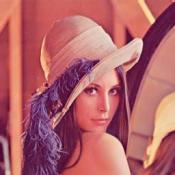
\includegraphics[width=7cm]{images/rgb.jpg}
			\end{figure} \\
			\hline
		\end{tabular}
	\end{adjustbox}
	\captionof{figure}{Contoh Citra Digital \cite{gonzalez}}
	\label{img:CitraDigital}
\end{table}

Suatu citra dapat bersifat kontinu sehubungan dengan koordinat x dan y, dan juga dalam intensitas. Untuk mengubahnya menjadi bentuk digital, harus dicoba fungsi dalam koordinat dan intensitas. \textit{Sampling} adalah proses untuk menentukan warna pada piksel tertentu pada citra dari sebuah gambar yang kontinu. Pada proses \textit{sampling} biasanya dicari warna rata-rata dari gambar analog yang kemudian dibulatkan. Proses \textit{sampling} sering juga disebut proses digitalisasi. \textit{Sampling} merupakan bagian dari metodologi statistika. Adakalanya, dalam proses \textit{sampling}, warna rata-rata yang didapat di relasikan ke level warna tertentu. Contohnya apabila dalam citra hanya terdapat 16 tingkatan warna abu-abu, maka nilai rata-rata yang didapat dari proses sampling harus diasosiasikan ke 16 tingkatan tersebut. Proses mengasosiasikan warna rata-rata dengan tingkatan warna tertentu disebut dengan kuantisasi.
\\ 

\subsection{Pengolahan Citra}
Pengolahan citra adalah salah satu cabang dari ilmu informatika (Komputer). Pengolahan citra berfokus pada usaha untuk melakukan transformasi suatu citra/gambar menjadi citra lain dengan menggunakan teknik tertentu. Berikut ini merupakan langkah-langkah yang umumnya dilakukan dalam merancang sebuah sistem pengolahan citra dan pengenalan pola:

\begin{table}[H]
	\small
	\begin{adjustbox}{width=1\textwidth}
		\begin{tabular}{| p {14cm} |}
			\hline
			\begin{figure}[H]
				\centering
				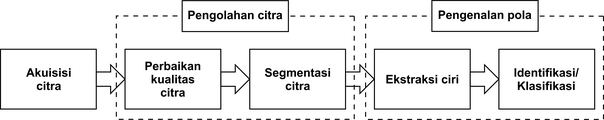
\includegraphics[width=14cm]{images/pencit}
			\end{figure} \\
			\hline
		\end{tabular}
	\end{adjustbox}
	\captionof{figure}{Proses Pengolahan Citra dan Pengenalan Pola}
	\label{img:pencit}
\end{table}

Operasi yang dilakukan untuk mengubah suatu citra menjadi citra lain dapat dikategorikan berdasarkan tujuan transformasi maupun cakupan operasi yang dilakukan terhadap citra. Berdasarkan tujuan transformasi operasi pengolahan citra dikategorikan menjadi peningkatan kualitas citra (\textit{Image Enhancement}) dan pemulihan citra (image restoration). Operasi peningkatan kualitas citra bertujuan untuk meningkatkan fitur tertentu pada citra. Sedangkan operasi pemulihan citra bertujuan untuk mengembalikan kondisi citra pada kondisi yang diketahui sebelumnya akibat adanya \textit{noise} yang menyebabkan penurunan kualitas citra. Berdasarkan cakupan operasi yang dilakukan terhadap citra, operasi pengolahan citra dikategorikan menjadi operasi titik, lokal, dan global. 

Operasi titik merupakan operasi yang dilakukan terhadap setiap piksel pada citra yang keluarannya hanya ditentukan oleh nilai piksel itu sendiri. Operasi titik dapat dibagi menjadi tiga macam, yaitu berdasarkan intensitas, geometri, dan gabungan keduanya. Contoh operasi titik berdasar intensitas adalah operasi pengambangan (\textit{thresholding}) yaitu membuat citra biner, operasi negatif (\textit{negative image}) yaitu membuat citra negatif, pemotongan citra (\textit{clipping}), dan pencerahan citra (\textit{image brightening}) yaitu menambahkan atau mengurangi konstanta untuk memperbaiki kecerahan pada citra. Operasi lokal merupakan operasi yang dilakukan terhadap setiap piksel pada citra yang keluarannya dipengaruhi oleh piksel tersebut dan piksel lainnya dalam suatu daerah tertentu. Salah satu contoh dari operasi berbasis lokal adalah operasi konvolusi untuk mendeteksi tepi (\textit{edge detection}) an pelembutan citra (\textit{image smoothing}). Operasi global merupakan operasi yang dilakukan tehadap setiap piksel pada citra yang keluarannya ditentukan oleh keseluruhan piksel yang membentuk citra. Contoh operasi global adalah operasi penyetaraan histogram untuk meningkatkan kualitas citra.\\

\subsection{\textit{Preprocessing}}
\textit{Preprocessing} merupakan proses pengolahan data asli sebelum tahapan pengolahan data. Proses ini bertujuan agar data siap untuk diproses ke tahap ektraksi fitur. Preprocessing memiliki tujuan untuk menghilangkan derau, memperjelas fitur, mengubah ukuran citra, dan konversi data. Contoh dari \textit{preprocessing} yaitu pengabuan citra (\textit{grayscaling}), binerisasi citra, \textit{croping} citra, dan \textit{resize} citra \cite{gonzalez}.\\ 

\subsubsection{Pengabuan Citra}
Citra \textit{grayscale} adalah suatu citra yang hanya memiliki warna berupa tingkat keabuan. Citra \textit{grayscale} digunakan karena membutuhkan sedikit informasi yang diberikan pada tiap piksel dibandingkan dengan citra berwarna sehingga dalam \textit{grayscale} image hanya membutuhkan nilai intensitas tunggal dibandingkan dengan citra berwarna membutuhkan tiga intensitas untuk tiap pikselnya. Intensitas dari citra \textit{grayscale} disimpan dalam 8 bit integer yang memberikan 256 kemungkinan yang mana dimulai dari level 0 sampai dengan 255 (0 untuk hitam dan 255 untuk putih) \cite{gonzalez}. Gambar \ref{img:grayscale} merupakan contoh dari citra \textit{grayscale}.

\begin{table}[H]
	\small
	\begin{adjustbox}{width=1\textwidth}
		\begin{tabular}{| p {14cm} |}
			\hline
			\begin{figure}[H]
				\centering
				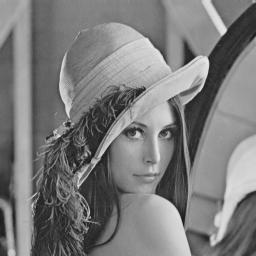
\includegraphics[width=7cm]{images/grayscale.jpg}
			\end{figure} \\
			\hline
		\end{tabular}
	\end{adjustbox}
	\captionof{figure}{Contoh Citra \textit{Grayscale} \cite{gonzalez}}
	\label{img:grayscale}
\end{table}

Persamaan pengabuan citra dapat dilihat pada persamaan \ref{eq:grayscale} dengan \textit{R} melambangkan intensitas warna merah, \textit{G} untuk intensitas warna hijau, dan \textit{B} untuk intensitas warna biru. 

\begin{table}[H]
	\begin{adjustbox}{width=1\textwidth}
		\begin{tabular}{|p{13.55cm}|}
			\hline
			\begin{equation}
			Gray value = 0.299 R + 0.587 G + 0.114 B
			\label{eq:grayscale}
			\end{equation}\\
			\hline
		\end{tabular}
	\end{adjustbox}
\end{table}

Persamaan \ref{eq:grayscale} menyimpulkan bahwa persentase warna hijau yang paling besar karena manusia cenderung lebih sensitif terhadap perubahan warna hijau yang memiliki panjang gelombang sekitar 500-570 nm, merah, lalu biru, dan merupakan rekomendasi dari \textit{International Telecommunication Union Radiocommunication Sector}.\\

\subsubsection{Citra Biner}
Citra biner (\textit{binary image}) adalah citra yang hanya mempunyai dua nilai derajat keabuan yaitu hitam dan putih. Citra biner bernilai 1 untuk objek dan 0 untuk latar belakang. Citra biner sering kali digunakan karena mempercepat waktu proses dan memperkecil penggunaan memori\cite{munir}. Meskipun komputer saat ini dapat memproses citra hitam-putih (\textit{grayscale}) maupun citra berwarna, namun citra biner masih tetap dipertahankan keberadaannya. 

\begin{table}[H]
	\small
	\begin{adjustbox}{width=1\textwidth}
		\begin{tabular}{| p {14cm} |}
			\hline
			\begin{figure}[H]
				\centering
				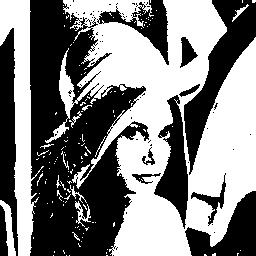
\includegraphics[width=7cm]{images/biner.jpg}
			\end{figure} \\
			\hline
		\end{tabular}
	\end{adjustbox}
	\captionof{figure}{Contoh Citra Biner \cite{gonzalez}.}
	\label{img:binary}
\end{table}

Sama seperti citra \textit{grayscale}, citra biner juga merupakan citra yang hanya memiliki satu kanal warna. Citra biner memiliki kedalaman bit sebesar 1-bit. \textit{Thresholding} adalah metode untuk mengubah citra \textit{grayscale} menjadi citra biner sehingga objek dapat dipisahkan dari \textit{background}. Untuk mendapat nilai \textit{threshold} yang adaptif menggunakan metode Otsu. Nilai intensitas warna pada setiap piksel citra biner dibagi menjadi 2$\land$1 = 2 warna yaitu warna hitam yang dinyatakan oleh nilai 0 dan warna putih yang dinyatakan oleh nilai 1. Persamaan yang digunakan untuk mengkonversi nilai piksel citra \textit{grayscale} menjadi biner pada metode \textit{thresholding} adalah:

\begin{table}[H]
	\small
	\begin{adjustbox}{width=1\textwidth}
		\begin{tabular}{|p{13.55cm}|}
			\hline
			\begin{equation} \label{eqn:biner}
			\displaystyle
			g(x,y) = \left\{\begin{array}{l}1, jika f(x,y) \ge T \\0, jika f(x,y) < T\end{array}\right.
			\end{equation} \\
			\hline
		\end{tabular}
	\end{adjustbox}
\end{table}

\noindent
\renewcommand{\arraystretch}{1}
\begin{tabularx}{\textwidth}{lll}
	\hline
	Keterangan: \\
	$g(x,y)$ & : & citra biner\\
	$f(x,y)$ & : & citra \textit{grayscale}\\
	$T$ & : & \textit{treshold}\\
	\hline
\end{tabularx}
\vspace{4.5pt} 

Citra biner digunakan saat proses penentuan ROI. ROI yang berupa citra biner digunakan untuk menandai lokasi dimana mobil akan melaju. ROI yang digunakan berupa template dari dataset yang diperoleh.\\

\subsubsection{\textit{Otsu Tresholding}}
Tujuan dari metode Otsu adalah membagi histogram citra gray level kedalam dua daerah yang berbeda secara otomatis tanpa membutuhkan bantuan pengguna untuk memasukkan nilai ambang. Pendekatan yang dilakukan oleh metode otsu adalah dengan melakukan analisis diskriminan yaitu menentukan suatu variabel (nilai ambang atau \textit{threshold}) yang dapat membedakan antara dua atau lebih kelompok yang muncul secara alami. Analisis Diskriminan akan memaksimumkan nilai ambang agar dapat membagi objek latar depan (\textit{foreground}) dan latar belakang (\textit{background}).

Langkah  awal  yang harus  dilakukan  adalah  membuat  histogram.  Dari histogram dapat diketahui jumlah piksel untuk setiap tingkat  keabuan.  Tingkat  keabuan  citra  dinyatakan dengan i sampai dengan L. Level ke i dimulai dari 1, yaitu  piksel  0.  Untuk L,  maksimal  level  adalah  256 dengan piksel bernilai 255. Nilai  ambang  yang  akan  dicari  dari  suatu  citra \textit{grayscale} dinyatakan dengan k. Nilai kberkisar antara 0  sampai  dengan L - 1,  dengan  nilai L = 256  (simbol histogram adalah Pi) \cite{otsu}. Jadi probabilitas setip piksel pada level ke i dinyatakan dengan persamaan berikut. 

\begin{table}[H]
	\small
	\begin{adjustbox}{width=1\textwidth}
		\begin{tabular}{|p{13.55cm}|}
			\hline
			\begin{equation} \label{eqn:otsu1}
			\displaystyle
			P_{i} = \frac{n_{i}}{N}
			\end{equation} \\
			\hline
		\end{tabular}
	\end{adjustbox}
\end{table}

\noindent
\renewcommand{\arraystretch}{1}
\begin{tabularx}{\textwidth}{lll}
	\hline
	Keterangan: \\
	$P_{i}$ & : & probabilitas piksel ke-i\\
	$n_{i}$ & : & jumlah piksel dengan tingkat keabuan i\\
	$N$ & : & total jumlah piksel pada citra\\
	\hline
\end{tabularx}
\vspace{4.5pt}

Langkah   selanjutnya   mencari   nilai   jumlah kumulatif, rerata  kumulatif  dan  intensitas  global. mencari  nilai  tersebut  dapat  melihat  persamaan  \eqref{eqn:otsu2}, persamaan \eqref{eqn:otsu3}, dan persamaan \eqref{eqn:otsu4}.

\begin{table}[H]
	\small
	\begin{adjustbox}{width=1\textwidth}
		\begin{tabular}{|p{13.55cm}|}
			\hline
			\begin{equation} \label{eqn:otsu2}
			\displaystyle
			\omega (k) = \sum\limits_{i=0}^{k} p_{i}
			\end{equation} 
			
			\begin{equation} \label{eqn:otsu3}
			\displaystyle
			\mu (k) = \sum\limits_{i=0}^{k} i . p_{i}
			\end{equation}
			 
			\begin{equation} \label{eqn:otsu4}
			\displaystyle
			\mu _{T} (k) = \sum\limits_{i=0}^{L-1} i . p_{i}
			\end{equation}\\
			\hline
		\end{tabular}
	\end{adjustbox}
\end{table}

\noindent
\renewcommand{\arraystretch}{1}
\begin{tabularx}{\textwidth}{lll}
	\hline
	Keterangan: \\
	$k$ & : &  tingkat level keabuan  dimana  setiap  rentang  piksel  akan  dihitung\\
	$\omega (k)$ & : & jumlah kumulatif\\
	$\mu (k)$ & : & rerata Kumulatif\\
	$\mu _{T} (k)$ & : & rerata Intensitas Global\\
	\hline
\end{tabularx}
\vspace{4.5pt}

Langkah selanjutnya adalah menentukan varian antar kelas  (\textit{between class variance}).

\begin{table}[H]
	\small
	\begin{adjustbox}{width=1\textwidth}
		\begin{tabular}{|p{13.55cm}|}
			\hline
			\begin{equation} \label{eqn:otsu5}
			\displaystyle
			\sigma_{B}^{2} (k)  = \frac{[\mu _{T}\omega (k)-\mu (k)] ^2}{\omega (k)[1 - \omega (k)]}
			\end{equation} \\
			\hline
		\end{tabular}
	\end{adjustbox}
\end{table}

\noindent
\renewcommand{\arraystretch}{1}
\begin{tabularx}{\textwidth}{lll}
	\hline
	Keterangan: \\
	$\sigma_{B}^{2}$ & : & nilai ambang\\
	$k$ & : &  tingkat level keabuan  dimana  setiap  rentang  piksel  akan  dihitung\\
	$\omega (k)$ & : & jumlah kumulatif\\
	$\mu (k)$ & : & rerata Kumulatif\\
	$\mu _{T} (k)$ & : & rerata Intensitas Global\\
	\hline
\end{tabularx}
\vspace{4.5pt}

Hasil  dari  perhitungan \textit{between class variance} dicari   nilai   maksimal.   Nilai   yang   paling   besar digunakan  sebagai \textit{threshold} atau  nilai  ambang  (k), dengan persamaan \eqref{eqn:otsu6}.

\begin{table}[H]
	\small
	\begin{adjustbox}{width=1\textwidth}
		\begin{tabular}{|p{13.55cm}|}
			\hline
			\begin{equation} \label{eqn:otsu6}
			\displaystyle
			\sigma_{B}^{2} (k\star)  = max_{1 \leq x \leq L} \sigma_{B}^{2}
			\end{equation} \\
			\hline
		\end{tabular}
	\end{adjustbox}
\end{table}

\noindent
\renewcommand{\arraystretch}{1}
\begin{tabularx}{\textwidth}{lll}
	\hline
	Keterangan: \\
	$\sigma_{B}^{2}$ & : & nilai ambang maksimal\\
	$\omega (k)$ & : & jumlah kumulatif\\
	$\mu (k)$ & : & rerata Kumulatif\\
	$\mu _{T} (k)$ & : & rerata Intensitas Global\\
	$\sigma_{B}^{2}$ & : & nilai ambang\\
	$k$ & : &  tingkat level keabuan  dimana  setiap  rentang  piksel  akan  dihitung\\
	\hline
\end{tabularx}
\vspace{4.5pt}

\textit{Between class variance} bertujuan untuk mencari nilai   ambang dari sebuah citra \textit{grayscale}, nilai ambang atau \textit{threshold} digunakan sebagai nilai acuan untuk mengubah citra \textit{grayscale} ke citra biner. Setiap citra memiliki nilai ambang yang berbeda-beda.
\\

\subsubsection{Derau}
Derau (\textit{Noise}) merupakan piksel yang mengganggu kualitas citra. Derau dapat disebabkan oleh gangguan fisis (optik) pada alat akuisisi maupun secara disengaja akibat proses pengolahan yang tidak sesuai \cite{gonzalez}. Beberapa gangguan mungkin saja terjadi saat pengambilan citra, seperti kamera tidak fokus atau munculnya bintik-bintik yang bisa terjadi karena proses pengambilan gambar yang tidak sempurna. Setiap gangguan pada citra dinamakan derau, yang tidak hanya terjadi karena ketidak sempurnaan dalam proses pengambilan citra, tetapi dapat disebabkan juga oleh noda kotoran yang terjadi pada citra setelah pengambilan citra. Contohnya adalah bintik hitam atau putih yang muncul secara acak yang tidak diinginkan di dalam citra. Bintik acak ini disebut dengan derau \textit{salt and pepper}. \textit{Salt and Pepper} merupakan \textit{noise} yang terkadang muncul pada citra. \textit{Noise} ini dapat terjadi karena adanya gangguan pada citra, misalnya temperatur. \textit{Salt and Pepper} pada citra berupa piksel hitam putih yagn tersebar seperti pada gambar \ref{fig:ContohDerau}.

\begin{table}[H]
	\small
	\begin{adjustbox}{width=1\textwidth}
		\begin{tabular}{| p {14cm} |}
			\hline
			\begin{figure}[H]
				\centering
				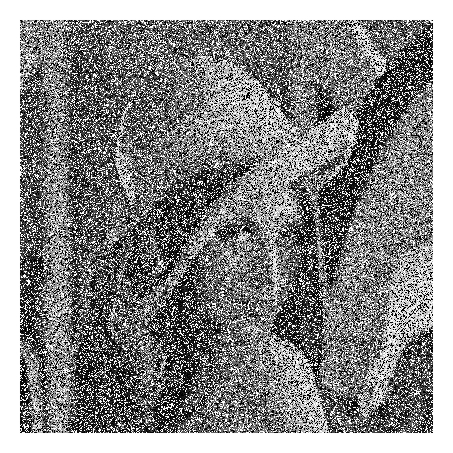
\includegraphics[width=7cm]{images/noise_snp}
			\end{figure} \\
			\hline
		\end{tabular}
	\end{adjustbox}
	\captionof{figure}{Contoh Derau \textit{Salt and Pepper} \cite{gonzalez}.}
	\label{fig:ContohDerau}
\end{table}

\subsubsection{Segmentasi Citra}
Segmentasi citra adalah membagi suatu citra menjadi wilayah - wilayah yang homogen \cite{gonzalez}. Tahapan ini bertujuan untuk mempartisi citra menjadi bagian-bagian pokok yang mengandung informasi penting. Misalnya, memisahkan objek dan latar belakang. Segmentasi terdiri dari \textit{downsampling}, penipisan dan deteksi tepian. 

Tahap \textit{downsampling} merupakan proses untuk menurunkan jumlah piksel dan menghilangkan sebagian informasi dari citra. Dengan resolusi citra yang tetap, downsampling menghasilkan ukuran citra yang lebih kecil. \textit{Thinning} (penipisan) adalah proses mengurangi suatu obyek didalam citra digital menjadi ukuran yang minimum (objek (\textit{region}) direduksi menjadi rangka (\textit{skeleton})). \textit{Thinning} hanya digunakan pada citra biner dan menghasilkan citra biner lain sebagai outputnya . \textit{Thinning} bertujuan untuk mengurangi bagian yang tidak perlu (\textit{redudant}) sehingga hanya dihasilkan informasi yang penting saja. Pola hasil penipisan harus tetap menyerupai bentuk pola asal. Penentuan tepian suatu objek dalam citra merupakan salah satu wilayah pengolahan citra digital yang paling awal dan paling banyak diteliti. Proses ini seringkali ditempatkan sebagai langkah pertama dalam aplikasi segmentasi citra, yang bertujuan untuk mengenali objek-objek yang terdapat dalam citra ataupun konteks citra secara keseluruhan. Deteksi tepi berfungsi untuk mengidentifikasi garis batas (\textit{boundary}) dari suatu objek yang terdapat pada citra.

Algoritme segmentasi didasarkan pada 2 buah karakteristik nilai derajat kecerahan citra, yaitu: \textit{discontinuity} dan \textit{similarity}. Pada \textit{discontinuity}, citra dipisahkan/dibagi atas dasar perubahan yang mencolok dari derajad kecerahannya. Aplikasi yang umum adalah untuk deteksi titik, garis, area, dan sisi citra. Pada \textit{similarity} didasarkan atas \textit{thresholding, region growing}, dan \textit{region spiltting and merging}.
\\

\subsubsection{Deteksi Tepi}
Deteksi tepi (\textit{Edge detection}) adalah operasi yang dijalankan untuk mendeteksi garis tepi (\textit{edges}) yang membatasi dua wilayah citra homogen yang memiliki tingkat kecerahan yang berbeda \cite{gonzalez}. Tujuannya adalah untuk mengubah citra 2D menjadi bentuk kurva. Metode yang banyak digunakan untuk proses deteksi tepi adalah metode Robert, Prewitt, Sobel, dan Canny. Hasil dari metode - metode deteksi tepi dapat dilihat pada gambar \ref{fig:ContohDeteksiTepi}.

\begin{table}[H]
	\small
	\begin{adjustbox}{width=1\textwidth}
		\begin{tabular}{| p {14cm} |}
			\hline
			\begin{figure}[H]
				\centering
				\subfloat[ ]{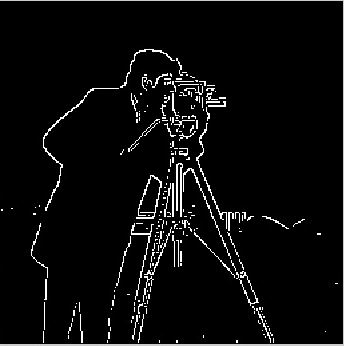
\includegraphics[width = 5cm]{images/roberts}} 
				\subfloat[ ]{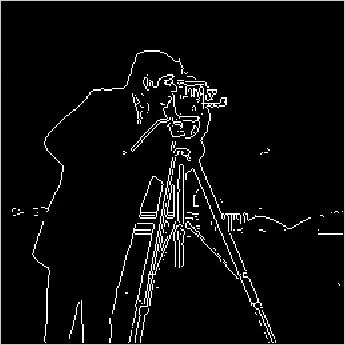
\includegraphics[width = 5cm]{images/prewitt}}\\
				\subfloat[ ]{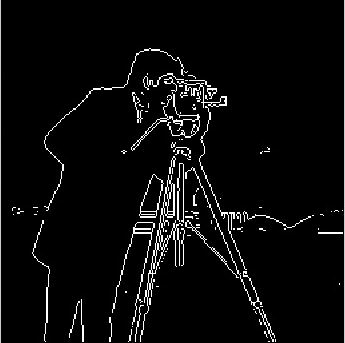
\includegraphics[width = 5cm]{images/sobel}}
				\subfloat[ ]{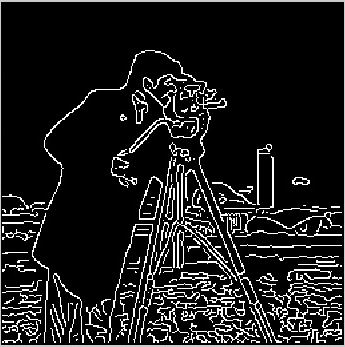
\includegraphics[width = 5cm]{images/canny}} 
			\end{figure} \\
			\hline
		\end{tabular}
	\end{adjustbox}
	\captionof{figure}{Contoh Deteksi Tepi \cite{gonzalez}. (a) Robert (b) Prewitt (c) Sobel (d) Canny}
	\label{fig:ContohDeteksiTepi}
\end{table}

Metode pada deteksi tepi terletak pada penggunaan kernel yang berbeda. Metode Sobel merupakan pengembangan metode robert dengan menggunakan filter HPF yang diberi satu angka nol penyangga. Metode ini mengambil prinsip dari fungsi laplacian dan gaussian yang dikenal sebagai fungsi untuk membangkitkan HPF. Kelebihan dari metode sobel ini adalah kemampuan untuk mengurangi noise sebelum melakukan perhitungan deteksi tepi. Kernel filter yang digunakan dalam metode Sobel ini adalah: 

\begin{center}
	\begin{tabular}{ c c c}
		$
		x = 
		\left[ \begin{array}{rcl}
		-1 & -2 & -1 \\ 
		0 & 0 & 0 \\
		1 & 2 & 1 \end{array} \right]
		\mbox{~dan~}
		y =
		\left[ \begin{array}{rcl}
		-1 & 0 & 1 \\ 
		-2 & 0 & 2 \\
		-1 & 0 & 1 \end{array} \right]
		$
	\end{tabular}
\end{center}

%Kemudian kernel untuk deteksi garis diagonal menggunakan:

%\begin{center}
%	\begin{tabular}{ c c c}
%		$
%		X = 
%		\left[ \begin{array}{rcl}
%		-0 & 1 & 2 \\ 
%		-1 & 0 & 1 \\
%		-2 & -1 & 0 \end{array} \right]
%		\mbox{~dan~}
%		Y =
%		\left[ \begin{array}{rcl}
%		-2 & -1 & 0 \\ 
%		-1 & 0 & 1 \\
%		0 & 1 & 2 \end{array} \right]
%		$
%	\end{tabular}
%\end{center}

Koordinat x didefinisikan di sini sebagai peningkatan pada arah horizontal, dan koordinat y didefinisikan sebagai peningkatan pada arah vertikal. Pada setiap titik dalam gambar, perkiraan gradien yang dihasilkan dapat dikombinasikan untuk memberikan besarnya gradien menggunakan rumus:

\begin{table}[H]
	\small
	\begin{adjustbox}{width=1\textwidth}
		\begin{tabular}{|p{13.55cm}|}
			\hline
			\begin{equation} \label{eqn:sobel}
			\displaystyle
			|G| = \sqrt{G_{x}^{2}+G_{y}^{2}}
			\end{equation} \\
			\hline
		\end{tabular}
	\end{adjustbox}
\end{table}

\noindent
\renewcommand{\arraystretch}{1}
\begin{tabularx}{\textwidth}{lll}
	\hline
	Keterangan: \\
	$G$ & : & gradien\\
	$G_{x}$ & : & arah sumbu X\\
	$G_{y}$ & : & arah sumbu Y\\
	\hline
\end{tabularx}
\vspace{4.5pt}

\subsubsection{\textit{Region of Interest} (ROI)}
\textit{Region   of  Interest}   adalah  suatu   bagian   dari   citra   yang   dipilih   untuk kemudian  diproses. Daerah  tersebut  dibedakan  dengan  menggunakan klasifikasi dan \textit{masking}.  Jika  piksel pada   \textit{mask}  tidak   nol,   maka   pemrosesan   citra   dilakukan. Sebaliknya jika piksel pada \textit{mask} sama dengan nol, proses tidak dijalankan. Setelah  daerah yang diinginkan ditemukan, daerah  tersebut  ditandai dengun kotak  untuk  membatasi  daerah  yang akan  dikenali. Dalam  \textit{Region  of  Interest}, citra  dapat  didefinisikan lebih  dari  satu  region (bagian). \textit{Region  of Interest}  sangat membantu untuk  segmentasi dalam  pemrosesan citra karena  dengan  menggunakan teknik  ini  citra  atau  obyek  dapat  lebih mudah dikenali. Karena obyek sudah akan dibagi dalam \textit{region - region} tertentu  sesuai dengan citra obyeknya. \textit{Region  of  Interest} membantu dalam mengurangi penggunaan memori.\\

\subsubsection{\textit{Sliding Window}}
Pada bidang \textit{computer vision}, \textit{sliding window} merupakan sebuah daerah persegi atau persegi panjang yang memiliki ukuran tertentu dan akan bergeser dengan jarak tertentu secara berurutan ke seluruh daerah citra. Tahap ini dilakukan untuk memproses citra lokal secara bergantian dan pada umumnya digunakan untuk prooses pencarian dari suatu citra. Ukuran dari \textit{window} dan jarak perpindahan antar \textit{window} yang digunakan tergantung dari masalah yang akan diselesaikan maka biasanya ukuran tersebut disesuaikan dengan ukuran objek pada citra. Ukuran \textit{window} yang optimal adalah \textit{window} yang dapat mencakup keseluruhan objek, tidak terlalu besar atau kecil, oleh karena itu, perlu dilakukan alanilis objek citra agar mendapatkan keseluruhan objek. Sama halnya dengan jarak perpindahan antar \textit{window}, bila terlalu besar akan terdapat bagian citra yagn terlewat, bila terlalu kecil akan menyebabkan waktu komputasi yang lebih lama. 

\subsection{Ekstraksi Fitur}
Ekstraksi fitur merupakan suatu pengambilan ciri (fitur) dari suatu bentuk yang nantinya nilai yang didapatkan akan dianalisis untuk proses selanjutnya \cite{gonzalez}. Ekstraksi fitur bertujuan untuk mencari daerah fitur yang signifikan pada gambar. Ekstraksi fitur dilakukan dengan cara menghitung jumlah titik atau piksel yang ditemui dalam setiap pengecekan, dimana pengecekan dilakukan dalam berbagai arah pengecekan pada koordinat kartesian dari citra digital yang dianalisis, yaitu vertikal, horizontal. Ciri yang telah diekstrak kemudian digunakan sebagai parameter / nilai masukan untuk membedakan antara objek satu dengan lainnya pada tahapan identifikasi/ klasifikasi. Ekstraksi fitur terbagi menjadi tiga macam yaitu ekstraksi fitur bentuk, ekstraksi fitur tekstur, ekstraksi fitur warna.

Bentuk dari suatu objek adalah karakter permukaan yang diwakili oleh garis dan kontur. Fitur bentuk dikategorikan bergantung pada teknik yang digunakan berdasarkan daerah (\textit{region-based}) dan berdasarkan batas (\textit{boundary-based}). Teknik berdasarkan daerah (\textit{region-based}) menggambarkan bentuk wilayah dengan menggunakan karakteristik internal, contohnya adalah piksel yang berada dalam suatu wilayah. Sedangkan teknik berdasarkan batas (\textit{boundary-based}) menggambarkan bentuk daerah dengan menggunakan karakteristik eksternal, contohnya adalah piksel sepanjang batas objek.

Pada ekstraksi fitur tekstur, fitur pembeda adalah tekstur yang merupakan karakteristik penentu pada citra. Teknik statistik yang terkenal untuk ekstraksi fitur adalah matriks gray level co-occurrence. Teknik tersebut dilakukan dengan melakukan pemindaian untuk mencari jejak derajat keabuan setiap dua buah piksel yang dipisahkan dengan jarak d dan sudut $\theta$ yang tetap. Biasanya sudut yang digunakan adalah 0, 45, 90, dan 135. Sedangkan pada ekstraksi fitur warna, ciri pembeda adalah warna. Biasanya ekstraksi fitur ini digunakan pada citra berwarna yang memiliki komposisi warna RGB (red, green, blue).
\\

\subsubsection{\textit{Histogram of Oriented Gradients}}
\textit{Histogram of Oriented Gradients} (HOG) merupakan metode ekstraksi fitur bentuk berupa garis dengan memperhatikan distribusi gradien intensitas lokal atau arah tepi. Dalam praktiknya ini dilakukan dengan membagi jendela gambar menjadi wilayah spasial kecil ("sel"). Untuk setiap sel mengumpulkan histogram 1-D lokal dari arah gradien atau orientasi tepi atas piksel sel. Sel dikumpulkan menjadi blok untuk dinormalisasi. Blok deskriptor hasil normalisasi disebut deskriptor HOG \cite{dalal}. Pertama akan dihitung gradien untuk setiap piksel pada citra dari sumbu x dan y dengan menggunakan : 

\begin{table}[H]
	\small
	\begin{adjustbox}{width=1\textwidth}
		\begin{tabular}{|p{13.55cm}|}
			\hline
			\begin{equation} \label{eqn:GradientH}
			\displaystyle
			G_{x}(x,y) = I(x+1,y) - I(x-1,y)
			\end{equation} 
			
			\begin{equation} \label{eqn:GradientV}
			\displaystyle
			G_{y}(x,y) = I(x,y+1) - I(x,y-1)
			\end{equation}\\
			\hline
		\end{tabular}
	\end{adjustbox}
\end{table}

\noindent
\renewcommand{\arraystretch}{1}
\begin{tabularx}{\textwidth}{lll}
	\hline
	Keterangan: \\
	$G_{x}(x,y)$ & : & gradien sumbu x\\
	$G_{y}(x,y)$ & : & gradien sumbu y\\
	$I(x,y)$ & : & nilai piksel citra dari baris x dan dan kolom y\\
	\hline
\end{tabularx}
\vspace{4.5pt}

Setelah mendapat gradien dari sumbu x dan y dari setiap piksel, besar nilai dan arah gradien dihitung menggunakan:
\begin{table}[H]
	\small
	\begin{adjustbox}{width=1\textwidth}
		\begin{tabular}{|p{13.55cm}|}
			\hline
			\begin{equation} \label{eqn:BesarGradien}
			\displaystyle
			G(x,y) = \sqrt{G_{x}(x,y)^{2}+G_{y}(x,y)^{2}}
			\end{equation} 
			
			\begin{equation} \label{eqn:ArahGradien}
			\displaystyle
			\theta(x,y) = \arctan\frac{G_{y}(x,y)}{G_{x}(x,y)}
			\end{equation}\\
			\hline
		\end{tabular}
	\end{adjustbox}
\end{table}

\noindent
\renewcommand{\arraystretch}{1}
\begin{tabularx}{\textwidth}{lll}
	\hline
	Keterangan: \\
	$G(x,y)$ & : & besar nilai gradien sumbu x dan y\\
	$\theta(x,y)$ & : & arah nilai gradien sumbu x dan y\\
	\hline
\end{tabularx}
\vspace{4.5pt}

Setiap piksel pada citra kemudian dibagi ke dalam sel, yang kemudian dihitung persebaran HOGnya menggunakan vote. Pertama, proses vote pada HOG dilakukan dengan membagi jumlah sudut gradien ke dalam jumlah \textit{orientation bin} untuk menentukan nilai - nilai dari \textit{bin}. Untuk setiap arah sudut gradien dari setiap piksel dalam sel dimasukkan ke dalam rentang \textit{orientation bin} yang sudah ditentukan. Besar nilai gradien kemudian dibagi dengan \textit{orientation bin} yang berhubungan. HOG dibuat untuk setiap sel.

Selanjutnya dilakukan normalisasi terhadap vote pada setiap \textit{bin} dalam sel. Normalisasi dilakukan dalam 1 blok dengan ukuran m x n sel. Metode untuk normalisasi terdapat sebanyak 4 buah meliputi: \textit{L2-Norm, L2-Hys, L1-sqrt, dan L1-norm}. Pada penelitian ini, akan digunakan normalisasi dengan metode \textit{L2-Norm} dengan persamaan:

\begin{table}[H]
	\small
	\begin{adjustbox}{width=1\textwidth}
		\begin{tabular}{|p{13.55cm}|}
			\hline
			\begin{equation} \label{eqn:normalisasi2}
			\displaystyle
			f =\sqrt{ \frac{v}{\sum\limits_{n=1}^{N} v}}
			\end{equation} \\
			\hline
		\end{tabular}
	\end{adjustbox}
\end{table}

\noindent
\renewcommand{\arraystretch}{1}
\begin{tabularx}{\textwidth}{lll}
	\hline
	Keterangan: \\
	$v$ & : & bobot vektor hasil \textit{L1-Sqrt} yang mewakili setiap \textit{bin}\\
	$i$ & : & nilai counter i sampai dengan N\\
	$N$ & : & total nilai \textit{bin} untuk normalisasi\\
	\hline
\end{tabularx}
\vspace{4.5pt}

Untuk algoritme rumus normalisasi L2-Hys merupakan algoritma mengikuti dari L2-Norm, namun dengan membatasi nilai maksimal hasil normalisasi sebesar 0,2.

Proses normalisasi blok dilakukan dengan sliding window yang melakukan proses dengan pergeseran sebesar 1x ukuran sel secara vertikal dan horizontal. Proses ini akan bersifat overlapping untuk beberapa sel yang dinormalisasi sehingga menimbulkan informasi yang redundan, namun akurasi yang dihasilkan justru semakin meningkat \cite{opencv}.
\\

\subsection{Klasifikasi}
Klasifikasi adalah sebuah proses untuk menemukan sebuah model yang menjelaskan dan membedakan konsep atau kelas data dengan tujuan memperkirakan kelas dari suatu objek yang kelasnya tidak diketahui \cite{steinwart}. 
\\ 

\subsubsection{\textit{Support Vector Machine}}
\textit{Support Vector Machines} (SVM) merupakan metode klasifikasi. SVM mengelompokkan fitur menjadi beberapa kelas menggunakan \textit{hyperplane} pada suatu ruang yang disebut \textit{feature space}.

\begin{table}[H]
	\small
	\begin{adjustbox}{width=1\textwidth}
		\begin{tabular}{| p {14cm} |}
			\hline
			\begin{figure}[H]
				\centering
				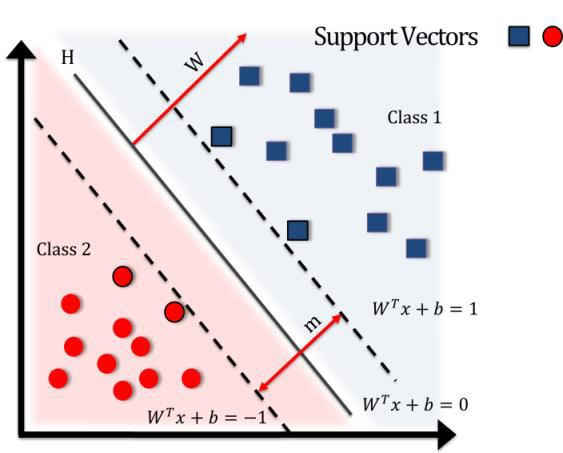
\includegraphics[width=6cm]{images/svm.jpg}
			\end{figure} \\
			\hline
		\end{tabular}
	\end{adjustbox}
	\captionof{figure}{Contoh \textit{Hyperplane} pada SVM \cite{bougharriou}.}
	\label{img:hyerplane_svm}
\end{table}
Berdasarkan contoh pada gambar \ref{img:hyerplane_svm}, \textit{hyperplane} merupakan sebuah indikator pemisah dimana ditentukan berdasarkan \textit{training} dengan margin tertinggi \cite{steinwart}. \textit{Hyperplane} yang optimal harus memenuhi persamaan berikut:
\begin{table}[H]
	\small
	\begin{adjustbox}{width=1\textwidth}
		\begin{tabular}{|p{13.55cm}|}
			\hline
			\begin{equation} 
			\label{eqn:hiperplane}
			w^T \cdot x + b = 0
			\end{equation}\\
			\hline
		\end{tabular}
	\end{adjustbox}
\end{table}

\noindent
\renewcommand{\arraystretch}{1}
\begin{tabularx}{\textwidth}{lll}
\hline
Keterangan: \\
$w$ & : & vektor berat\\
$.$ & : & perkalian vektor\\
$x$ & : & vektor input\\
$b$ & : & nilai bias\\
\hline
\end{tabularx}
\vspace{4.5pt}

Proses pemetaan dalam SVM menggunakan kernel, dan kernel yang biasanya digunakan adalah RBF (\textit{Radiant Basis Function}). Berikut rumus kernel RBF:
\begin{table}[H]
	\small
	\begin{adjustbox}{width=1\textwidth}
		\begin{tabular}{|p{13.55cm}|}
			\hline
			\begin{equation} 
			\label{eqn:jarakfitur}
			K(x,z) = e^{-((x-z)^2/(2\sigma^2)}
			\end{equation}\\
			\hline
		\end{tabular}
	\end{adjustbox}
\end{table}

\noindent
\renewcommand{\arraystretch}{1}
\begin{tabularx}{\textwidth}{lll}
	\hline
	Keterangan: \\
	$x  dan  z$ & : & pasangan dua data training\\
	$\sigma$ & : & konstanta\\
	\hline
\end{tabularx}
\vspace{4.5pt}

Klasifikasi non-linier dilakukan menggunakan persamaan:
\begin{table}[H]
	\small
	\begin{adjustbox}{width=1\textwidth}
		\begin{tabular}{|p{13.55cm}|}
			\hline
			\begin{equation}
			\label{eqn:rbfkernel} 
			f(x) = sign(\sum\limits_{i=1}^{m}\alpha_{i}y_{i}K()x,x_{i}+b)
			\end{equation}\\
			\hline
		\end{tabular}
	\end{adjustbox}
\end{table}

\noindent
\renewcommand{\arraystretch}{1}
\begin{tabularx}{\textwidth}{lll}
	\hline
	Keterangan: \\
	$\alpha_{i}$ & : & alpha\\
	$y_{i}$ & : & kelas\\
	$K(x,x_{i})$ & : & kernel matriks\\
	$b$ & : & bias\\
	\hline
\end{tabularx}
\vspace{4.5pt}

Jika nilai f(x) adalah 1, maka data tersebut akan masuk ke kelas positif. Sedangkan jika f(x) menunjukkan -1, maka data tersebut menunjukkan ke nilai kelas yang negatif.
\\

%\subsection{\textit{Confusion Matrix}}
%Confusion Matrix merupakan metode pengukuran yang akurat untuk mengevaluasi hasil klasifikasi. Dengan melakukan klasifikasi sebanyak C kelas, akan dihasilkan matriks berukuran CxC [15]. Ilustrasi (Gambar 2.11) menunjukkan kasus klasifikasi 2 buah kelas, sehingga matriks berukuran 2x2.
%\\

\subsection{\textit{Confusion Matrix}}
\textit{Confusion Matrix} merupakan sebuah tabel yang digunakan untuk mengukur performa dari suatu \textit{classifier} \cite{confusion-matrix}. Berikut ini merupakan gambar untuk menjelaskan \textit{confusion matrix}.
\begin{table}[H]
	\small
	\begin{adjustbox}{width=1\textwidth}
		\begin{tabular}{| p {14cm} |}
			\hline
			\begin{figure}[H]
				\centering
				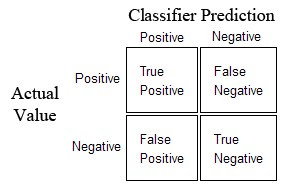
\includegraphics[width=7cm]{images/confusion_matrix.jpg}
			\end{figure} \\
			\hline
		\end{tabular}
	\end{adjustbox}
	\captionof{figure}{\textit{Confusion Matrix}}
	\label{img:confusionmatrix}
\end{table}
Contoh di atas merupakan confusion matrix untuk klasifikasi 2 kelas. Tabel memiliki 4 istilah yang akan dijelaskan sebagai berikut:

\begin{enumerate}
	\item True Positive (TP) : kondisi dimana data aktual bernilai positif dan prediksi dari klasifier bernilai positif.
	\item True Negative (TN): kondisi dimana data aktual bernilai negatif dan prediksi dari klasifier bernilai negatif.
	\item False Positive (FP): kondisi dimana data aktual bernilai negatif dan prediksi dari klasifier bernilai positif.
	\item False Negatif (FN): kondisi dimana data aktual bernilai positif dan prediksi dari klasifier bernilai negatif.
\end{enumerate}

Dari perhitungan di atas terdapat persamaan turunan lain yang bisa digunakan untuk menghitung performa dari \textit{classifier}.

\begin{enumerate}
	\item
	\textit{Accuracy}:  menghitung nilai prediksi yang benar oleh \textit{classifier}
	\begin{table}[H]
		\small
		\begin{adjustbox}{width=1\textwidth}
			\begin{tabular}{|p{13.55cm}|}
				\hline
				\begin{equation}
				Accuracy=(True Positives+True Negatives)/TotalData
				\end{equation}\\
				\hline
			\end{tabular}
		\end{adjustbox}
	\end{table}
	
	\item
	\textit{Misclassification Rate}: menghitung nilai kesalahan klasifikasi oleh \textit{classifier.} 
	\begin{table}[H]
		\small
		\begin{adjustbox}{width=1\textwidth}
			\begin{tabular}{|p{13.55cm}|}
				\hline
				\begin{equation}
				Misclassification\ Rate=(False Positives+False Negatives)/TotalData
				\end{equation}\\
				\hline
			\end{tabular}
		\end{adjustbox}
	\end{table}	
	
	\item
	\textit{True Positive Rate}: menghitung nilai prediksi bernilai positif ketika data aktual bernilai positif.
	\begin{table}[H]
		\small
		\begin{adjustbox}{width=1\textwidth}
			\begin{tabular}{|p{13.55cm}|}
				\hline
				\begin{equation}
				True \ Positive \ Rate\ (Recall)=True Positives/Actual Yes)
				\end{equation}\\
				\hline
			\end{tabular}
		\end{adjustbox}
	\end{table}
	
	\item
	\textit{False Positive Rate}: menghitung nilai prediksi positif ketika data aktual bernilai negatif.
	\begin{table}[H]
		\small
		\begin{adjustbox}{width=1\textwidth}
			\begin{tabular}{|p{13.55cm}|}
				\hline
				\begin{equation}
				False \ Positive \ Rate=False Positive/Actual No
				\end{equation}\\
				\hline
			\end{tabular}
		\end{adjustbox}
	\end{table}	
	
	\item
	\textit{Specificity}: menghitung nilai prediksi negatif ketika data aktual bernilai negatif. 
	\begin{table}[H]
		\small
		\begin{adjustbox}{width=1\textwidth}
			\begin{tabular}{|p{13.55cm}|}
				\hline
				\begin{equation}
				Specificity=True Negatives/Actual No
				\end{equation}\\
				\hline
			\end{tabular}
		\end{adjustbox}
	\end{table}
	
	\item
	\textit{Precision}: menghitung nilai prediksi positif yang benar.
	\begin{table}[H]
		\small
		\begin{adjustbox}{width=1\textwidth}
			\begin{tabular}{|p{13.55cm}|}
				\hline
				\begin{equation}
				Precision=True Positives/Predicted  Yes
				\end{equation}\\
				\hline
			\end{tabular}
		\end{adjustbox}
	\end{table}	
	
	\item
	\textit{Prevalence}: menghitung seberapa sering data aktual bernilai positif muncul.
	\begin{table}[H]
		\small
		\begin{adjustbox}{width=1\textwidth}
			\begin{tabular}{|p{13.55cm}|}
				\hline
				\begin{equation}
				Prevalence=Actual Yes/TotalData
				\end{equation}\\
				\hline
			\end{tabular}
		\end{adjustbox}
	\end{table}
	
\end{enumerate}

\subsection{Penggunaan \textit{Library}}
Berikut adalah penjelasan dari \textit{library} yang digunakan di dalam penelitian. \\
\subsubsection{OpenCV}
\textit{Library} yang digunakan adalah OpenCV untuk proses \textit{pre-processing} citra. OpenCV merupakan \textit{library open-source} yang banyak digunakan untuk penelitian terkait proses pengolahan citra dan \textit{computer vision}. 
\begin{small}
	\begin{longtable}{| p {0.5cm} | p {6cm} | p {6cm} |}
		\caption{Tabel fungsi \textit{Library} OpenCV} \\
		\hline
		\textbf{No} & \textbf{\textit{Function}} & \textbf{Deskripsi}\\
		\hline
		\endfirsthead
		
		\multicolumn{3}{c}{\textbf{\tablename~\thetable} \textit{Tabel fungsi \textit{Library} OpenCV} (Lanjutan)}\\
		\hline
		\textbf{No} & \textbf{\textit{Function}} & \textbf{Deskripsi}\\
		\endhead\noindent
		1 & Imgcodecs.imread(String filename) & Mengambil citra dari \textit{path} yang diisikan ke parameter.\\
		\hline
		2 & Imgproc.cvtColor(Mat src, Mat dst, int code) & Mengubah jenis warna pada citra sesuai yang diinginkan. Parameter fungsi ini terdiri dari Mat asal, Mat tujuan, dan \textit{code}. \textit{Code} digunakan untuk memilih tipe konversi citra tersebut, misal \textit{grayscale}.\\
		\hline
		3 & Imgproc.Canny(Mat image,Mat edges,double threshold1, double threshold2) & Fungsi ini digunakan untuk mendeteksi tepian pada citra menggunakan Canny.\\
		\hline
		4 & Imgproc.GaussianBlur(Mat src, Mat dst, Size ksize, double sigmaX) & Melakukan \textit{Gaussian Filter} terhadap citra yang dimasukkan ke dalam parameter dengan ukuran \textit{kernel} dan nilai \textit{sigma} yang diberikan.\\
		\hline
		5 & Imgproc.threshold(Mat src, Mat dst, double thresh, double maxval, int type) & Melakukan \textit{thresholding} terhadap seluruh nilai piksel dari citra yang dijadikan masukkan dengan nilai \textit{threshold}, nilai maksimum, serta jenis metode \textit{thresholding} yang digunakan, misalnya metode \textit{thresholding} Otsu.\\
		\hline
		6 & Imgproc.findContours(Mat image, List<MatOfPoint> contours, Mat hierarchy, int mode, int method) & Melakukan pencarian kontur terhadap citra yang dijadikan masukkan.\\
		\hline
		7 & Imgproc.contourArea(Mat contour) & Melakukan perhitungan luas area dari kontur yang diberikan.\\
		\hline
		8 & Imgproc.imwrite(String filename, Mat img) & Menyimpan citra yang diisikan ke parameter ke \textit{path} yang dijadikan tujuan penyimpanan.\\
		\hline
	\end{longtable}
\end{small}

\section{Tinjauan Studi}
Terdapat beberapa metode yang dapat digunakan untuk melakukan deteksi mobil pada citra digital. Tabel 2.1 akan menjelaskan tentang metode-metode tersebut beserta hasil dari
penerapannya.
\begin{small}
	\begin{longtable}{| p {0.5cm} | p {3cm} | p {3.5cm} | p {3.5cm} | p {3.5cm} |}
		\caption{Tabel Tinjauan Studi} \\
		\hline
		\textbf{No}  & \textbf{Judul}  & \textbf{Masalah}  & \textbf{Metode}  & \textbf{Hasil} \\
		\hline
		\endfirsthead
		\hline
		\textbf{No}  & \textbf{Judul}  & \textbf{Masalah}  & \textbf{Metode}  & \textbf{Hasil} \\
		\hline
		\endhead
		1  & Adhi Prahara, Murinto "Car Detection Based on Road Direction on Traffic		Surveillance Image" & Mendeteksi mobil dari semua sudut pandang kamera pengawas. & HOG, SVM & Area jalan diekstraksi untuk menentukan area deteksi dan arah jalanan digunakan untuk menentukan detektor mobil yang akan digunakan oleh Linear-Support Vector Machine (Linear-SVM). \\
		\hline
		2  & Daniel Neumann, Tobias Langner, Fritz Ulbrich, Dorothee Spitta1and Daniel Goehring "Online  Vehicle  Detection  using  Haar-like,  LBP  and  HOG  Feature  basedImage  Classifiers  with  Stereo  Vision  Preselection" & Membandingkan metode ekstraksi fitur. & Haar-like, LBP, dan HOG & Memberikan perbandingan penggunaan metode ekstraksi fitur antara Haar-like, LBP, dan HOG. \\
		\hline
		3  & A.Shakin Banu dan P. Vasuki "Video Based Vehicle Detection Using Morphological Operation and HOG Feature Extraction" & Penggunaan proses morfologi dan HOG untuk mendeteksi objek. & Morphological Operation, HOG & Hasil analisis menerangkan bahwa deteksi kendaraan menggunakan metode ini mencapai tingkat kesuksesan dengan akurasi sekitar 83 persen. \\
		\hline
		4  & G. Adhika dan R.R.W. Ken "Penerapan Histogram of Oriented Gradients, Principal Component Analysis, dan AdaBoost untuk Sistem Pengenalan Wajah" & Penggunaan proses HOG, PCA, dan AdaBoost untuk pengenalan wajah. & HOG, PCA, AdaBoost & Hasil analisis menerangkan bahwa pengenalan wajah menggunakan metode PCA dapat meningkatkan akurasi. \\
		\hline
	\end{longtable}
\end{small}

Pada penelitian yang dilakukan Adhi Prahara et al., mengusulkan framework dengan metode HOG dan SVM untuk mendeteksi mobil. Pertama, dataset dibagi menjadi data latih dan data uji. Data dikelompokkan berdasarkan sudut pandang (depan atau belakang, kiri atas atau kanan bawah, kanan atas atau kiri bawah, kiri atau kanan). Selanjutnya, untuk menentukan sudut pandang, dilakukan deteksi arah jalan. Terakhir, metode HOG dan SVM digunakan untuk deteksi mobil.

Pada penelitian yang dilakukan Daniel Neumann et al., menerapkan detektor DPM (DeformableParts Model), di mana bagian-bagian dari pola gambar dilatih dengan peningkatan resolusi oleh filter bagian. Untuk dapat mengidentifikasi kendaraan digunakan klasifikasi gambar dan melatihnya pada tampilan belakang kendaraan. Kemudian menerapkan berbagai algoritma \textit{computer vision} yang efisien.

Pada penelitian yang dilakukan A. Shakin Banu et al., mengusulkan framework dengan metode morphological operations dan HOG untuk mendeteksi mobil. Pertama, akan dilakukan pemilihan ROI (\textit{Region of Interest}) untuk mengurangi penggunaan memori. Berdasarkan hasil pre-procesing, citra akan diterapkan Sobel edge Detection sehingga didapatkan fitur gradien fungsi intensitas dari frame yang kemudian digunakan untuk perhitungan gradien. Terakhir, metode morphological operation akan dilakukan untuk menghapus objek yang tidak seharusnya terdeteksi, sehingga mengurangi piksel dalam frame. HOG kemudian diterapkan untuk ekstraksi fitur dan SVM untuk menentukan apakah mobil atau bukan.

Pada penelitian yang dilakukan G. Adhika et al., menjelaskan bahwa terdapat banyak faktor yang mempengaruhi hasil pengenalan seperti kualitas citra, ekspresi wajah dan kemiripan bentuk dari komponen wajah manusia dimana hal tersebut mempengaruhi fitur HOG yang dihasilkan. Penggunaan metode PCA meningkatkan akurasi dari HOG dan AdaBoost dari 86\% menjadi 96\% dengan ukuran sel sebesar 8, blok sebesar 16, dan bin sebesar 16.\\

\section{Tinjauan Objek}
Pada bagian ini akan dijelaskan mengenai objek terkait yang akan digunakan dalam
penelitian ini.\\

\subsection{Deteksi Mobil}
Mobil adalah kendaraan darat yang digerakkan oleh tenaga mesin, beroda empat atau lebih (selalu genap), biasanya menggunakan bahan bakar minyak (bensin atau solar) untuk menghidupkan mesinnya. Jenis mobil yang terdeteksi terdiri 3 golongan yaitu kendaraan kecil, kendaraan sedang, dan kendaraan besar.  Hasil yang diperoleh dapat dimanfaatkan untuk mengetahui lokasi kendaraan yang melewati jalan tersebut dalam suatu interval waktu tertentu. Citra mobil yang digunakan merupakan hasil citra dari sudut horizontal yang diambil dari dasbor mobil. Contoh citra mobil dan hasil visualisasi fitur HOG dapat dilihat pada gambar \ref{img:car}.
\begin{table}[H]
	\small
	\begin{adjustbox}{width=1\textwidth}
		\begin{tabular}{| p {14cm} |}
			\hline
			\begin{figure}[H]
				\centering
				\subfloat[ ]{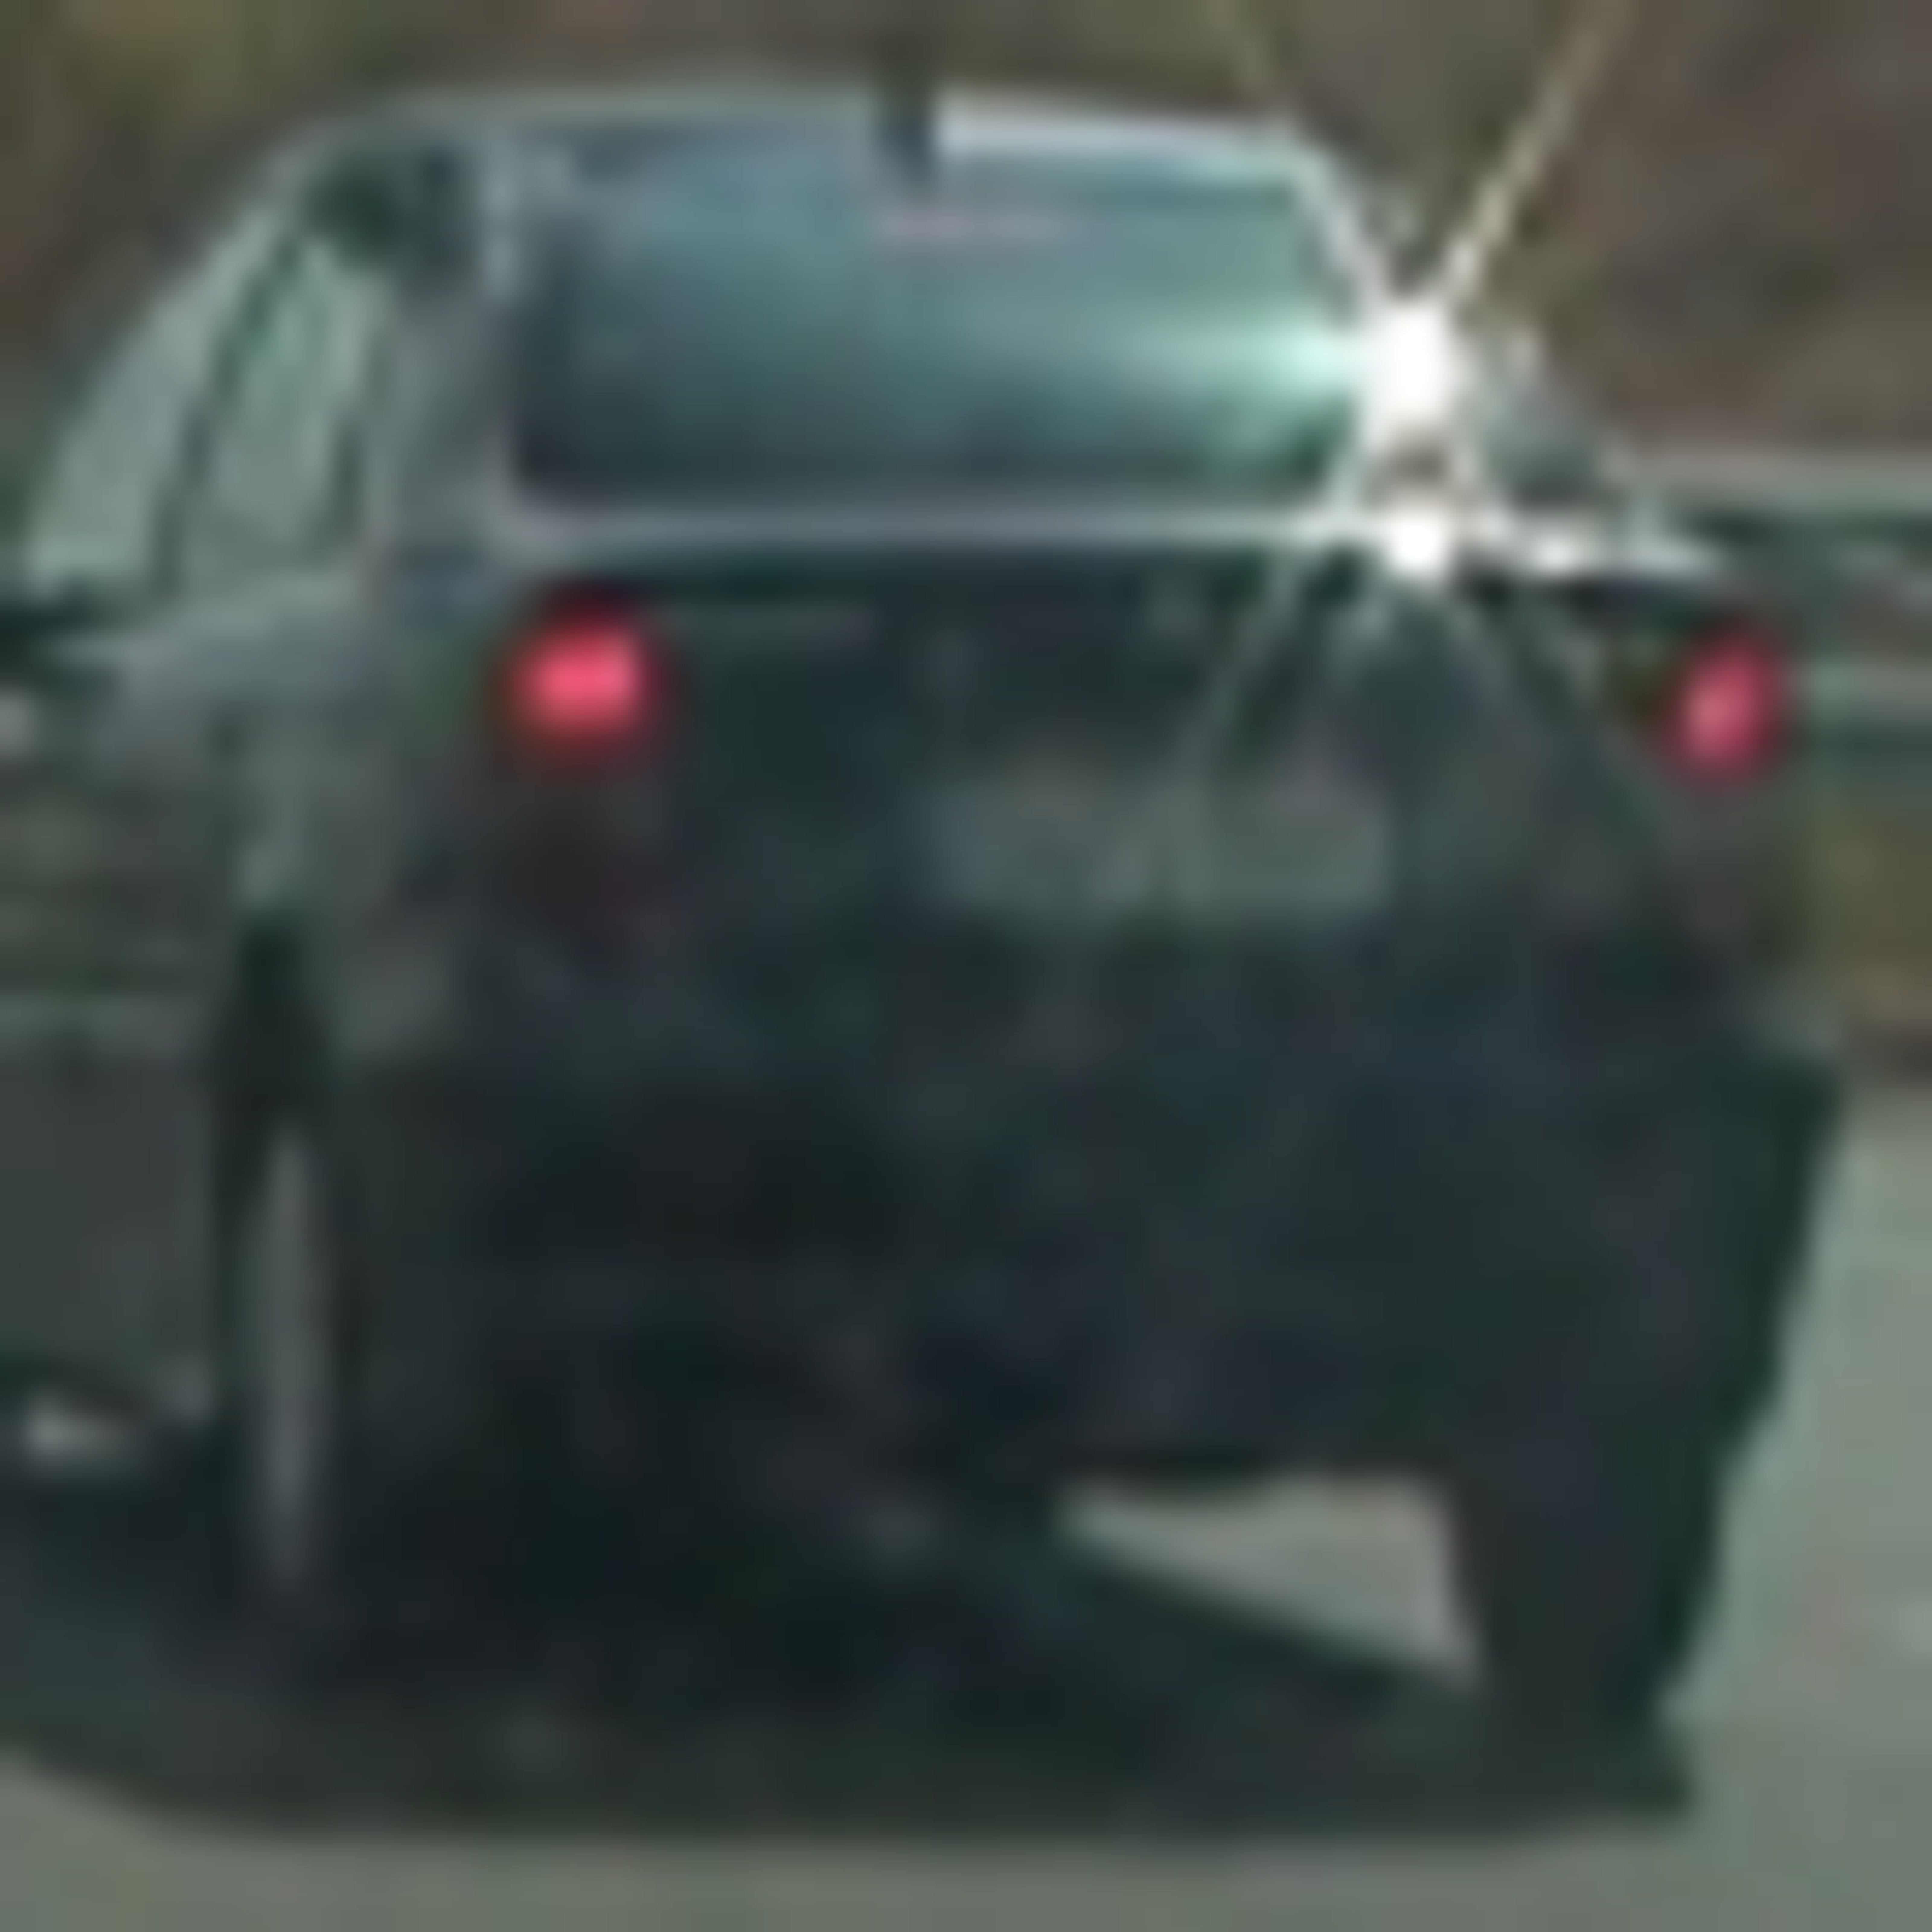
\includegraphics[width=7cm]{images/car.png}}
				\subfloat[ ]{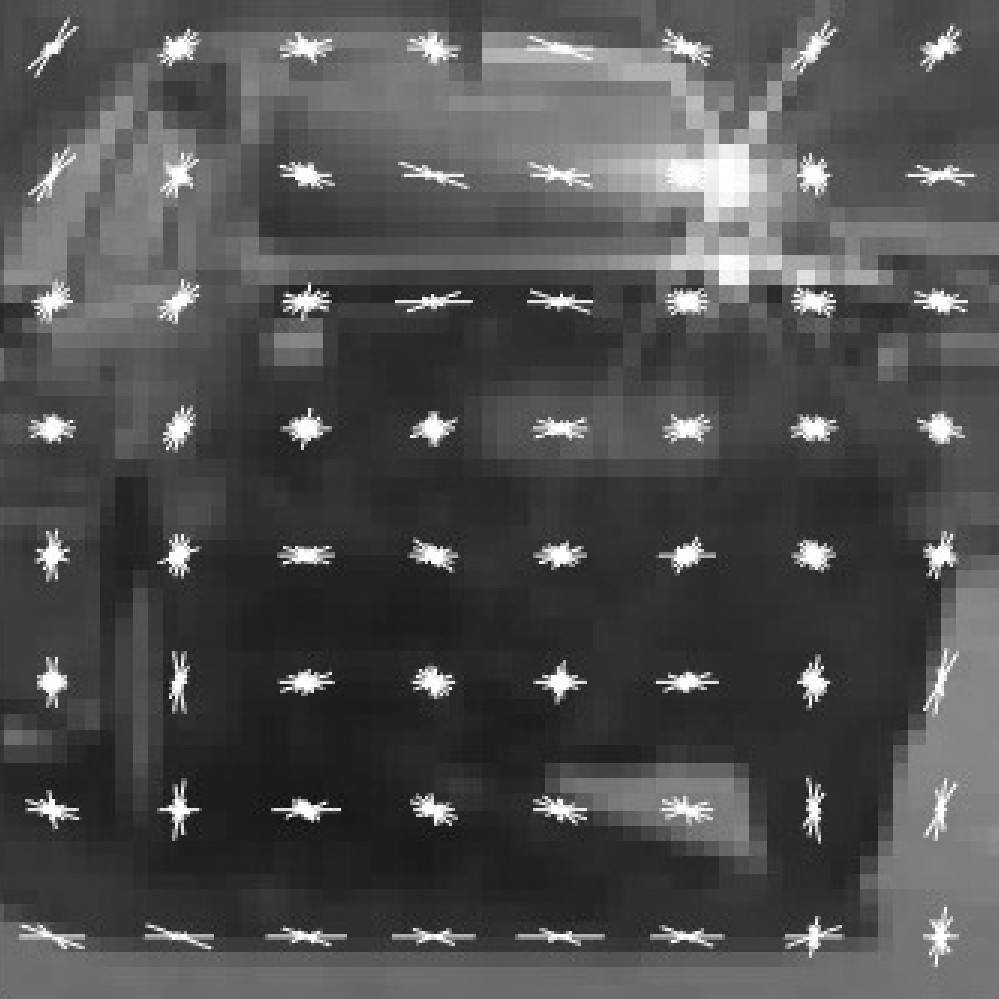
\includegraphics[width=7cm]{images/car_hog_gray8x8.jpg}}
			\end{figure} \\
			\hline
		\end{tabular}
	\end{adjustbox}
	\captionof{figure}{Citra Mobil nampak dari belakang. (a) Citra masukkan (b) Visualisasi fitur HOG}
	\label{img:car}
\end{table}
\newpage
%%-----------------------------------------------------------------------------%
\chapter{ANALISIS DAN PERANCANGAN SISTEM}
%-----------------------------------------------------------------------------%

%
\vspace{4.5pt}

Bab ini memaparkan analisis masalah yang diatasi berserta pendekatan dan alur kerja dari perangkat lunak yang dikembangkan, mengimplementasikan metode yang digunakan dan hasil yang akan ditampilkan.
\\
\section{Analisis Masalah}
Pada bab 1 telah dijelaskan bahwa penelitian sistem pengenalan mobil masih berkembang dan implementasinya memegang peranan penting dalam bidang transportasi. Pada penelitian ini, digunakan metode \textit{Histogram of Oriented Gradient} untuk mengekstraksi fitur yang sudah melalui tahap \textit{preprocessing}, kemudian dilakukan klasifikasi dengan menggunakan metode \textit{Support Vector Machine}. Klasifikasi yang dilakukan mengelompokkan objek menjadi 2 kelas yaitu mobil dan bukan mobil.

%Pada bab 1 telah dijelaskan bahwa mendeteksi manusia merupakan bidang yang masih berkembang dan implementasinya sangat dibutuhkan di berbagai bidang. Pada penelitian ini, penulis menggunakan citra RGB-D agar tetap memiliki hasil yang baik pada kondisi pencahayaan yang relatif gelap. Dengan menggunakan citra kedalaman akan sangat membantu dalam proses deteksi manusia dalam tahap awal, \textit{training}, ataupun tahap \textit{testing}. Penerapan \textit{Convolutional Neural Network} untuk mendeteksi manusia dan Kalman \textit{filter} untuk melacak manusia yang telah terdeteksi. Bagian tubuh manusia yang akan dideteksi adalah bagian tubuh atas sehingga tetap dapat mendeteksi manusia bila terdapat citra manusia yang tertutup atau hanya tampak sebagian.

Dataset yang digunakan terdiri dari 3 jenis dataset yang diambil dari sumber yang berbeda. Penelitian ini menggunakan \textit{dataset UIUC Car Image Database}, \textit{GTI Database}, dan \textit{KITTI Database}. Kemudian citra akan diubah menjadi format pgm. Citra yang digunakan  ialah citra \textit{grayscale} dengan \textit{depth bit} 8. Ukuran citra mobil yang digunakan berukuran 64 \time 64 piksel.

Penelitian   diawali   dengan   melakukan \textit{preprocessing dataset} menjadi citra \textit{grayscale} untuk mempermudah proses ekstraksi fitur. Setelah melalui tahap \textit{preprocessing}, selanjutnya adalah tahap pelatihan. Pada tahap ini, proses latih akan menggunakan metode HOG untuk mendapatkan fitur berupa gradien sudut yang direpresentasikan dalam bentuk fitur vektor. Kemudian hasil ekstraksi fitur tersebut akan dimasukkan ke dalam SVM untuk melakukan klasifikasi mobil dan bukan mobil. Hasil dari proses latih ini berupa matriks fitur yang akan digunakan untuk proses pegujian.

Tahap selanjutnya adalah melakukan proses pengujian. Proses pengujian akan melalui tahap yang sama dengan proses latih, namun pada inisialisasi fitur menggunakan hasil dari  fitur  yang  telah  didapatkan  sebelumnya. Pada tahap pengujian akan diperhatikan dampak antara penggunaan ROI dan tidak menggunakan ROI pada proses sliding windows. Hasil  deteksi  mobil adalah penandaan area dimana mobil terdeteksi.  Hasil deteksi  ini  akan  dibandingkan  dengan hasil deteksi yang  dibuat  manual  oleh  manusia.

Arsitektur yang digunakan  secara  garis  besar  masih  sama  dengan  arsitektur asli yang dibuat oleh Adhi Prahara \cite{prahara}, namun terdapat beberapa modifikasi untuk keperluan analisis parameter yang akan digunakan seperti orientasi, \textit{HOG channel}, ukuran sel dan ukuran blok.
\\

\section{Kerangka Pemikiran}
Berikut ini adalah kerangka pemikiran untuk melakukan deteksi mobil.\\

\begin{adjustbox}{width=1\textwidth}
	\begin{minipage}{\linewidth}
	\framebox[\textwidth]{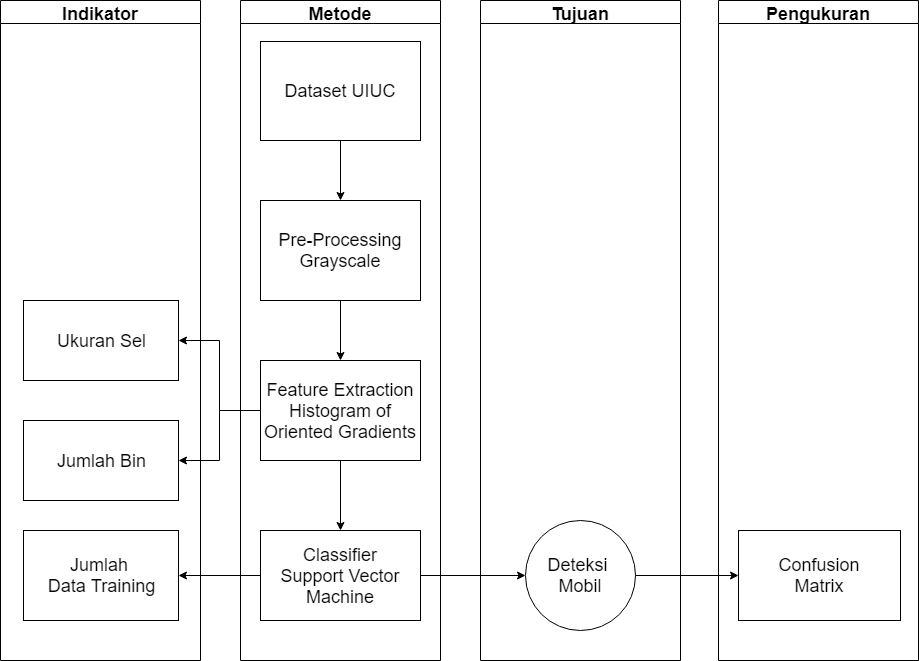
\includegraphics[width=14cm]{images/KerangkaPemikiran.png}}
	\captionof{figure}{Kerangka Pemikiran}
	\label{fig:KerangkaPemikiran}
\end{minipage}
\end{adjustbox}

Berdasarkan gambar \ref{fig:KerangkaPemikiran}, terdapat beberapa variabel indikator yang memengaruhi hasil dan perlu dilakukan penyesuaian meliputi ukuran sel, jumlah \textit{bin} yang menentukan batasan sudut yang digunakan, dan jumlah data \textit{training} untuk \textit{classifier} \textit{Support Vector Machine}. Ukuran sel akan mempengaruhi jumlah fitur. Semakin kecil ukuran sel, jumlah fitur akan bertambah. Penelitian ini bertujuan untuk melihat hasil akurasi dari deteksi mobil menggunakan \textit{confusion matrix}.\\

\section{Urutan Proses Global}
Dalam sistem pengenalan mobilterbagi atas dua proses yaitu proses \textit{training} dan proses \textit{testing}. Proses \textit{training} dilakukan untuk mendapatkan kelas dari objek yang akan dikenali. Proses \textit{testing} dilakukan untuk menghitung hasil yang berupa akurasi dari pengenalan mobil.

\begin{adjustbox}{width=1\textwidth}
	\begin{minipage}{\linewidth}
		\framebox[\textwidth]{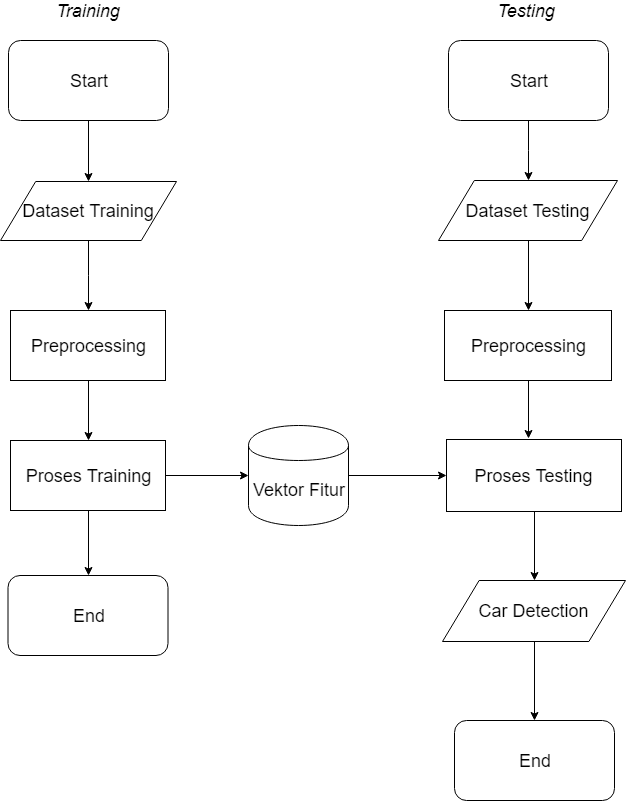
\includegraphics[width=10cm]{images/FlowchartGlobal.png}}
		\captionof{figure}{\textit{Flowchart Global} Sistem Pengenalan Mobil\\}
		\label{fig:FlowchartGlobal}
	\end{minipage}
\end{adjustbox}

Pada gambar \ref{fig:FlowchartGlobal}, dataset yang digunakan akan melalui tahap preprocessing untuk mempermudah proses ekstraksi fitur. Citra tersebut kemudian akan dibagi menjadi data latih dan data uji. Proses pelatihan akan menggunakan data latih untuk memperoleh fitur. Sedangkan proses pengujian akan menggunakan data uji dan fitur yang diperoleh dari tahap pelatihan. Hasil dari tahap pengujian adalah hasil deteksi mobil yang dibuat oleh sistem.
\\

\subsection{Proses \textit{Training}}

\begin{adjustbox}{width=1\textwidth}
	\begin{minipage}{\linewidth}
		\framebox[\textwidth]{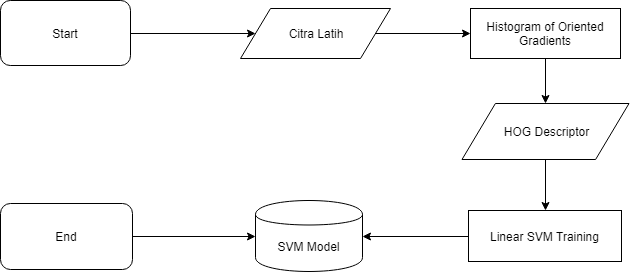
\includegraphics[width=14cm]{images/FlowchartTraining.png}}
		\captionof{figure}{\textit{Flowchart Training} Sistem Pengenalan Mobil\\}
		\label{fig:FlowchartTraining}
	\end{minipage}
\end{adjustbox}

Berikut ini adalah uraian dari \textit{flowchart} pada gambar \ref{fig:FlowchartTraining} yang dilakukan dalam penelitian ini:
\begin{enumerate}
\item Citra yang menjadi masukan yaitu dari data latih yang berisi kumpulan mobil. Citra mobil memiliki ukuran beragam dengan rentang ukuran lebar 200 - 300 piksel dan tinggi 100 - 200 piksel. Citra berupa \textit{grayscale} dengan arah pengambilan citra terdiri dari belakang.
\item \textit{Histogram of Oriented Gradient} berfungsi untuk mengambil fitur dari dari citra masukan. Hasil dari ekstraksi fitur menggunakan HOG adalah \textit{HOG descriptor}.\textit{HOG descriptor} mendeskripsikan distribusi dari gradien berarah pada suatu area citra.
\item Berdasarkan penelitian yang dilakukan oleh Dalal dan Triggs \cite{dalal}, \textit{HOG} menggunakan ukuran sel 8 $\times$ 8 piksel dan 16 $\times$ 16 piksel untuk ukuran blok kemudian \textit{bin} yang digunakan pada tahap pembuatan \textit{histogram} adalah 9 (dimulai dari 0 derajat hingga 180 derajat).
\item \textit{Support Vector Machine} (SVM) digunakan untuk klasifikasi fitur ke dalam 2 kelas (mobil dan bukan mobil) berdasar fitur yang sudah didapatkan. Hasil dari klasifikasi ini nantinya akan disimpan ke dalam bentuk berkas.\\
\end{enumerate}

\subsection{Proses \textit{Testing}}

\begin{adjustbox}{width=1\textwidth}
	\begin{minipage}{\linewidth}
		\framebox[\textwidth]{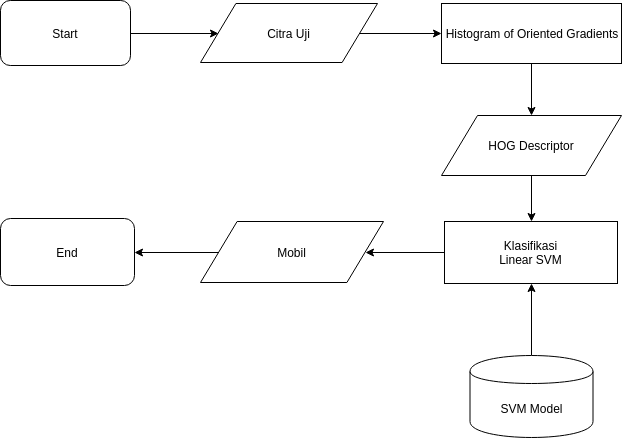
\includegraphics[width=14cm]{images/FlowchartTesting.png}}
		\captionof{figure}{\textit{Flowchart Testing} Sistem Pendeteksi Mobil\\}
		\label{fig:FlowchartTesting}
	\end{minipage}
\end{adjustbox}

\noindent Pada gambar \ref{fig:FlowchartTesting} terlihat alur proses \textit{testing}. Pada proses \textit{testing} terdapat beberapa proses yang sama seperti pada proses \textit{training}. Berikut adalah uraian dari \textit{flowchart} pada gambar \ref{fig:FlowchartTesting} yang dilakukan dalam penelitian ini:
\begin{enumerate}
\item Citra pengujian yang digunakan didapatkan dari \textit{dataset} dan \textit{www.youtube.com}, penggunaan dari dataset ini sesuai dengan perizinan dari institusi yang bersangkutan.
\item Citra yang akan menjadi input dari \textit{HOG} adalah citra hasil dari grayscale citra mobil yang sudah dilakukan pada tahapan \textit{preprocessing}.
\item Ukuran dari sel dan blok yang digunakan untuk proses ekstraksi fitur dengan menggunakan \textit{HOG} adalah sama dengan yang digunakan ketika pada tahap \textit{training}.
\item Pada tahap \textit{testing}, model SVM yang digunakan adalah berkas hasil keluaran dari SVM pada tahap \textit{training}.
\item Hasil keluaran akan berupa penandaan mobil yang berhasil dikenali oleh sistem.\\
\end{enumerate}

\section{Analisis Manual}
Bagian ini melakukan analisis tahapan proses dengan melakukan perhitungan manual. Analisis untuk proses pelatihan dan pembelajaran pada penelitian ini berjumlah yaitu mobil dan bukan mobil.\\

\subsection{\textit{Dataset}}
Dataset yang digunakan terdiri dari 3 jenis data latih yang diambil dari sumber yang berbeda. Penelitian ini menggunakan \textit{dataset UIUC Car Image Database}, \textit{GTI Database}, dan \textit{KITTI Database}. Arah pengambilan kamera untuk \textit{dataset} dilakukan dari posisi \textit{horizontal}.

Dataset \textit{UIUC Car Image Database} diperoleh dari \textit{http://cogcomp.org/Data/Car/}. Citra yang diambil dari \textit{dataset} merupakan citra \textit{grayscale} dengan 8 channel warna. Pada UIUC terdapat 1328 citra mobil. Dari total \textit{dataset} yang digunakan, terdiri dari 1050 citra latih dan 278 citra uji. Citra latih dibagi menjadi 2 macam, yaitu 550 citra mobil dan 500 bukan mobil. Citra mobil yang digunakan untuk citra latih diambil dari 2 arah yaitu kiri dan kanan. Citra uji terdiri dari beragam citra mobil yang terdiri dari 2 jenis yaitu 170 citra \textit{single-scale} dan 108 citra \textit{multi-scale} dengan ukuran panjang berkisar 100 piksel sampai 300 piksel dan lebar 75 piksel sampai 180 piksel. Pembagian data untuk pelatihan dan pengujian sudah dilakukan dari sumbernya. 

\begin{table}[H]
	\small
	\begin{adjustbox}{width=1\textwidth}
		\begin{tabular}{| p {14cm} |}
			\hline
			\begin{figure}[H]
				\centering
				\subfloat[ ]{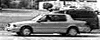
\includegraphics[width = 7cm]{images/DatasetUIUCLatihMobilKiri}} 
				\subfloat[ ]{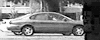
\includegraphics[width = 7cm]{images/DatasetUIUCLatihMobilKanan}} \\
				\subfloat[ ]{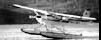
\includegraphics[width = 7cm]{images/DatasetUIUCLatihBukanMobil}}
				\subfloat[ ]{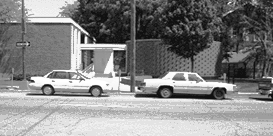
\includegraphics[width = 7cm]{images/DatasetUIUCUji}}\\
			\end{figure} \\
			\hline
		\end{tabular}
	\end{adjustbox}
	\captionof{figure}{Contoh \textit{Dataset UIUC}. (a) Data Latih Mobil (Kiri) (b) Data Latih Mobil (Kanan) (c) Data Latih Bukan Mobil (d) Data Uji}
	\label{fig:ContohUIUC}
\end{table}

\textit{Dataset GTI Database} diperoleh dari \textit{http://www.gti.ssr.upm.es/data/Vehicle\_database.html}. Citra yang diambil dari \textit{dataset} merupakan citra RGB dengan 24 channel warna. Untuk proses pelatihan dan pengujian, ada total 2826 data citra. Data latih yang digunakan diambil dari belakang mobil dengan 3 sudut pengambilan yaitu belakang lurus, belakang kiri, dan belakang kanan. Pengambilan citra dari belakang dilakukan dengan jarak dekat dan jarak jauh. Pembagian data untuk pelatihan dan pengujian dilakukan manual oleh peneliti.

\begin{table}[H]
	\small
	\begin{adjustbox}{width=1\textwidth}
		\begin{tabular}{| p {14cm} |}
			\hline
		\begin{figure}[H]
			\centering
			\subfloat[ ]{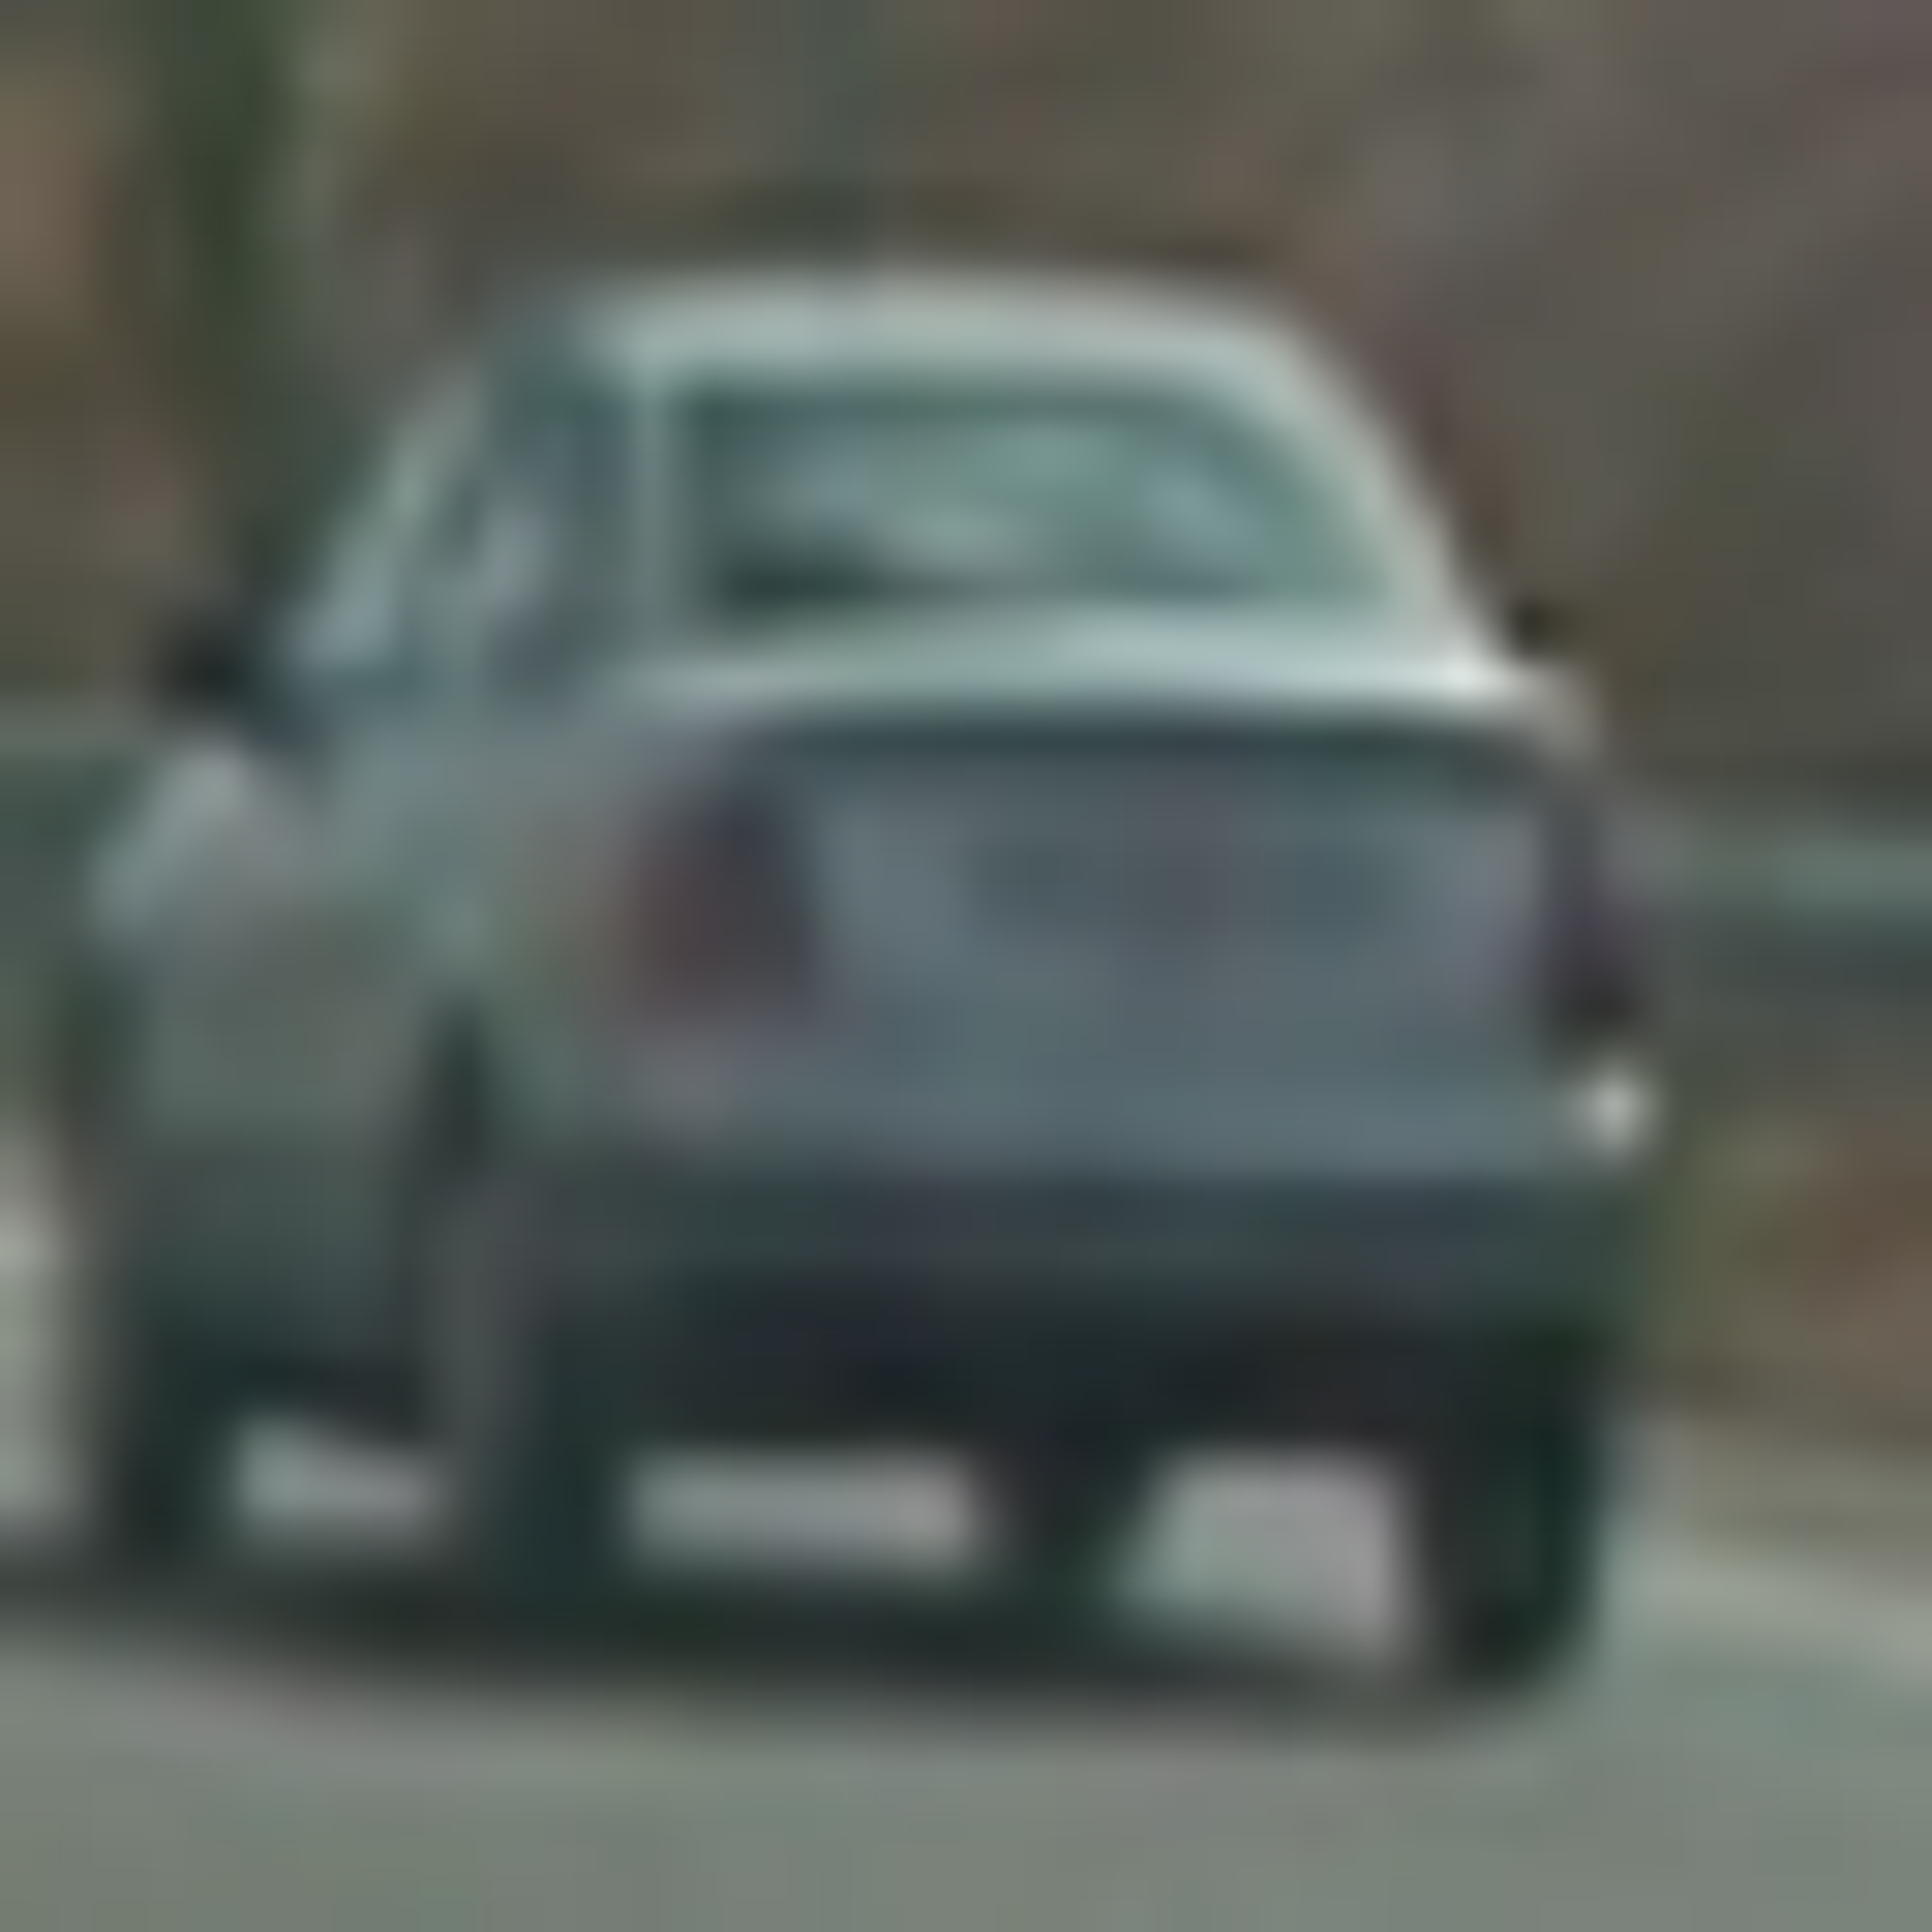
\includegraphics[width = 7cm]{images/DatasetGTILatihMobilKanan}}
			\subfloat[ ]{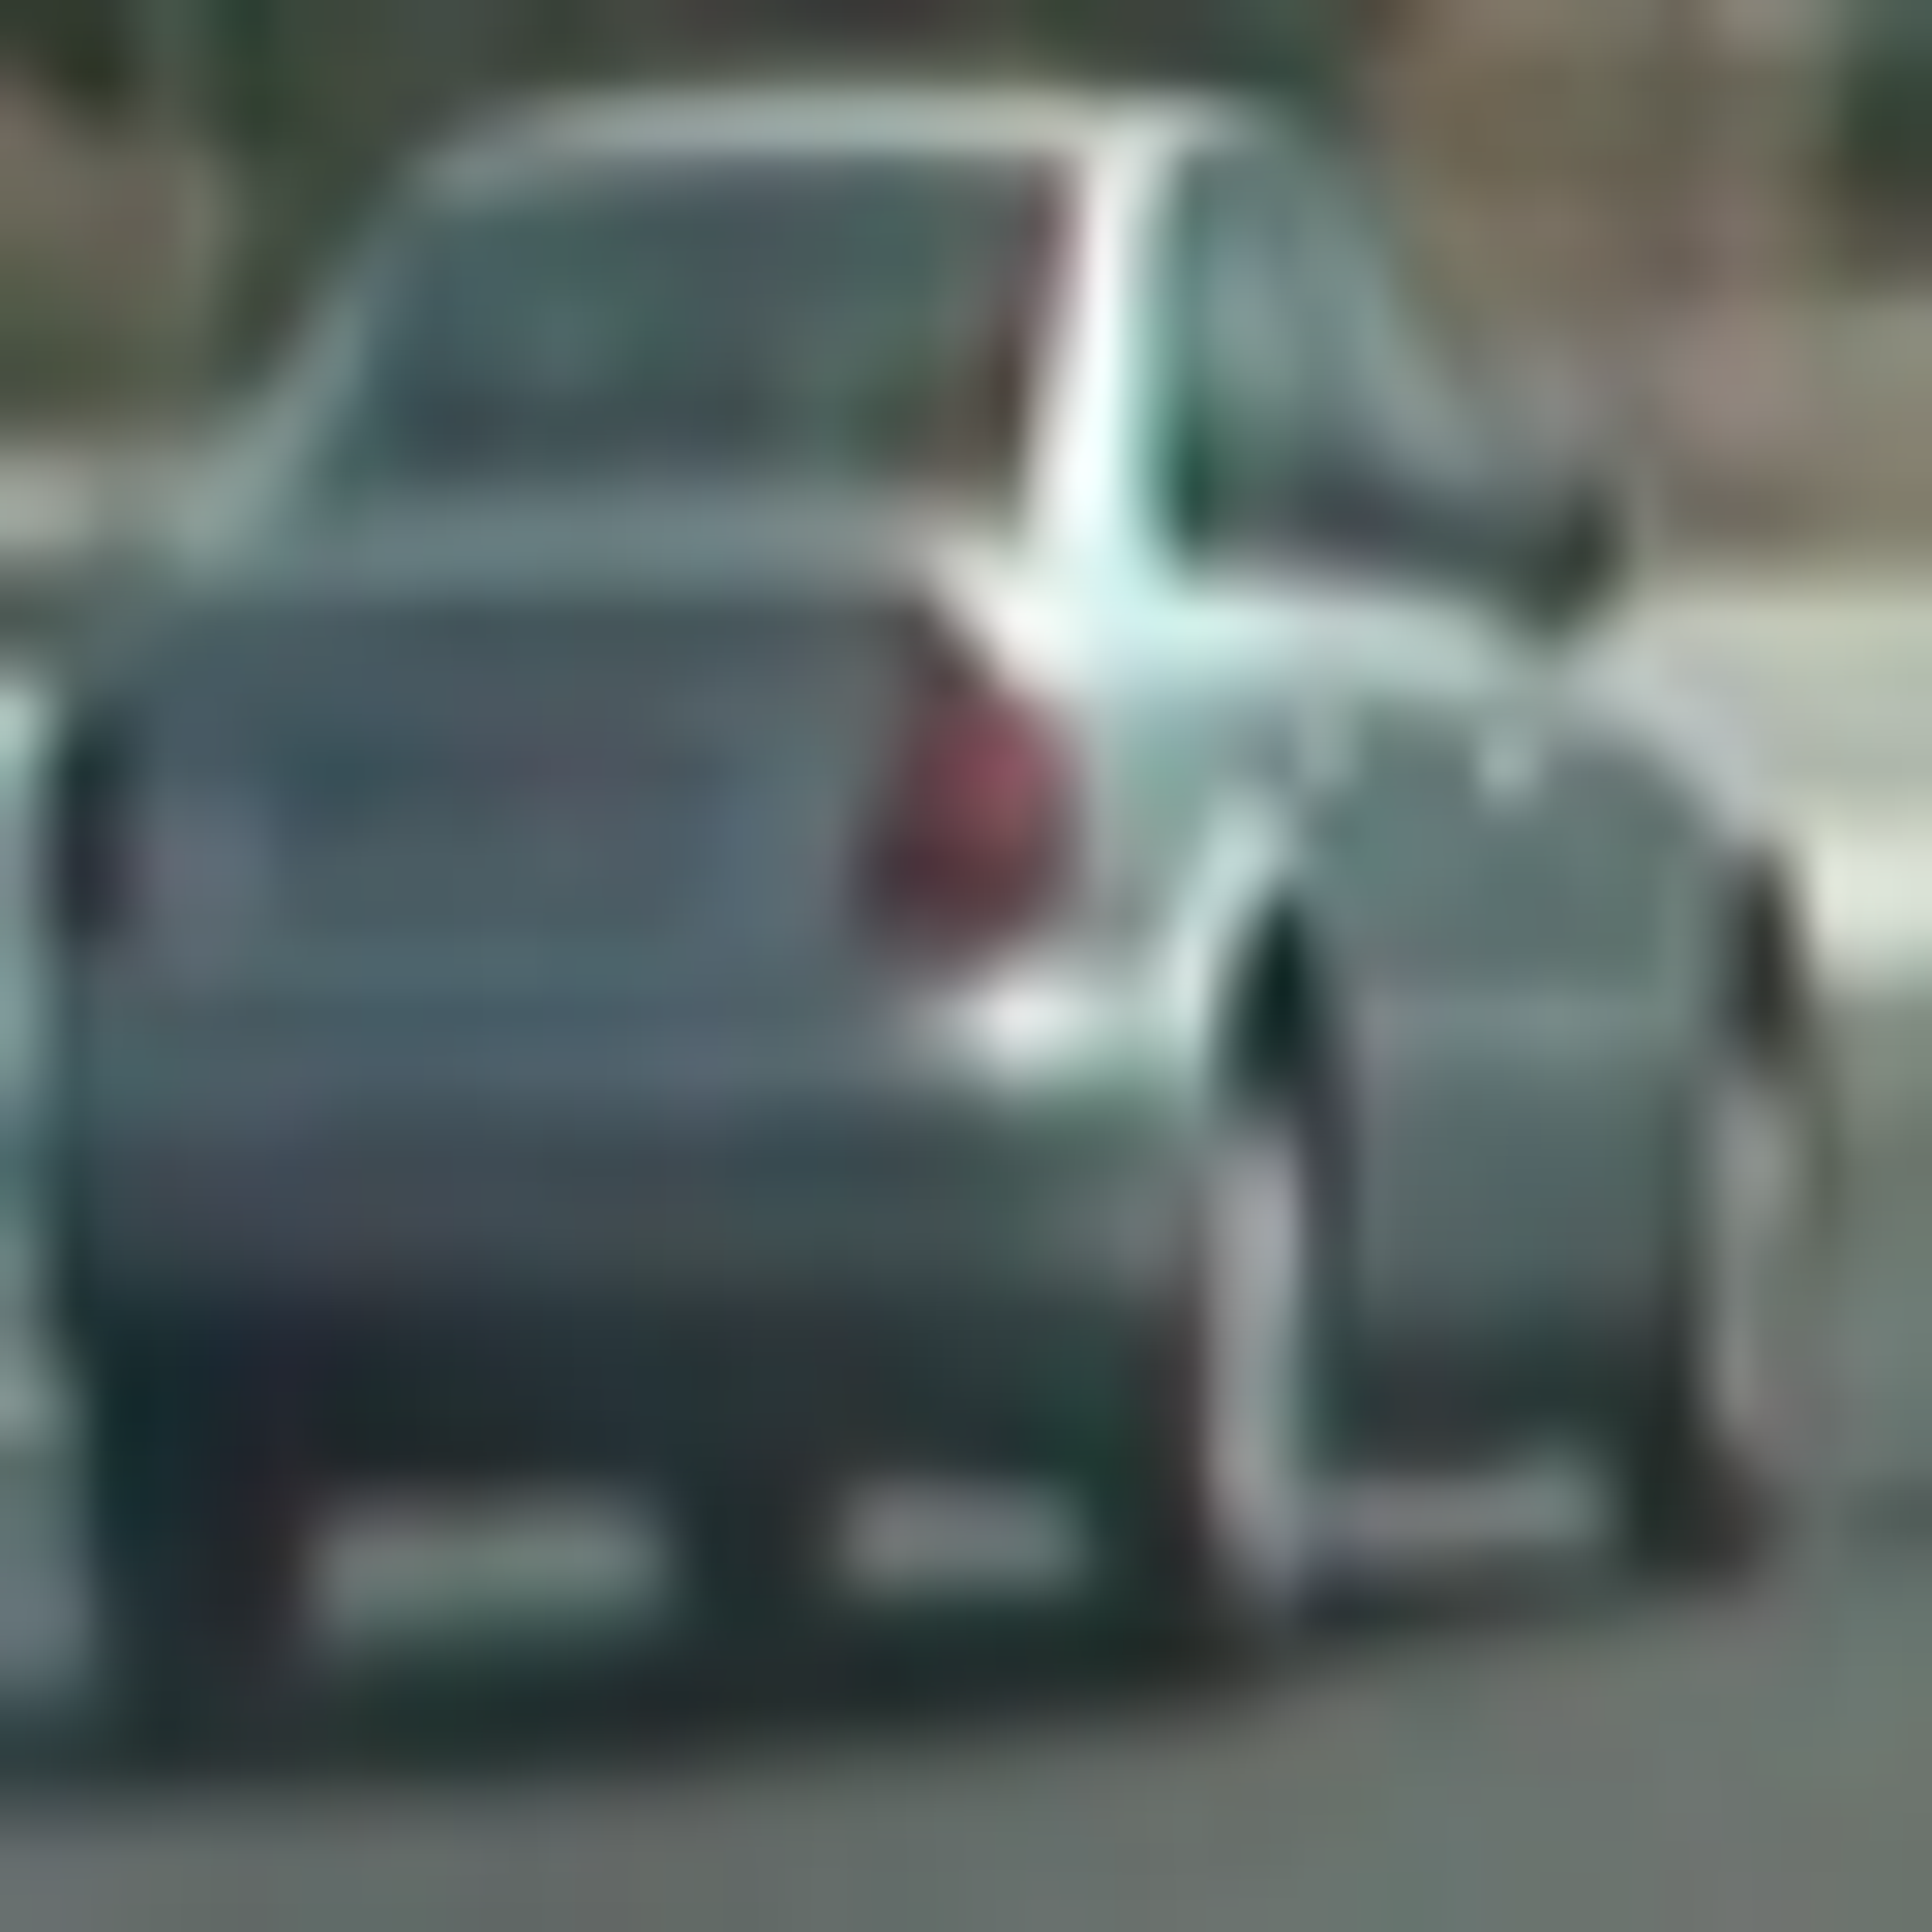
\includegraphics[width = 7cm]{images/DatasetGTILatihMobilKiri}}\\
			\subfloat[ ]{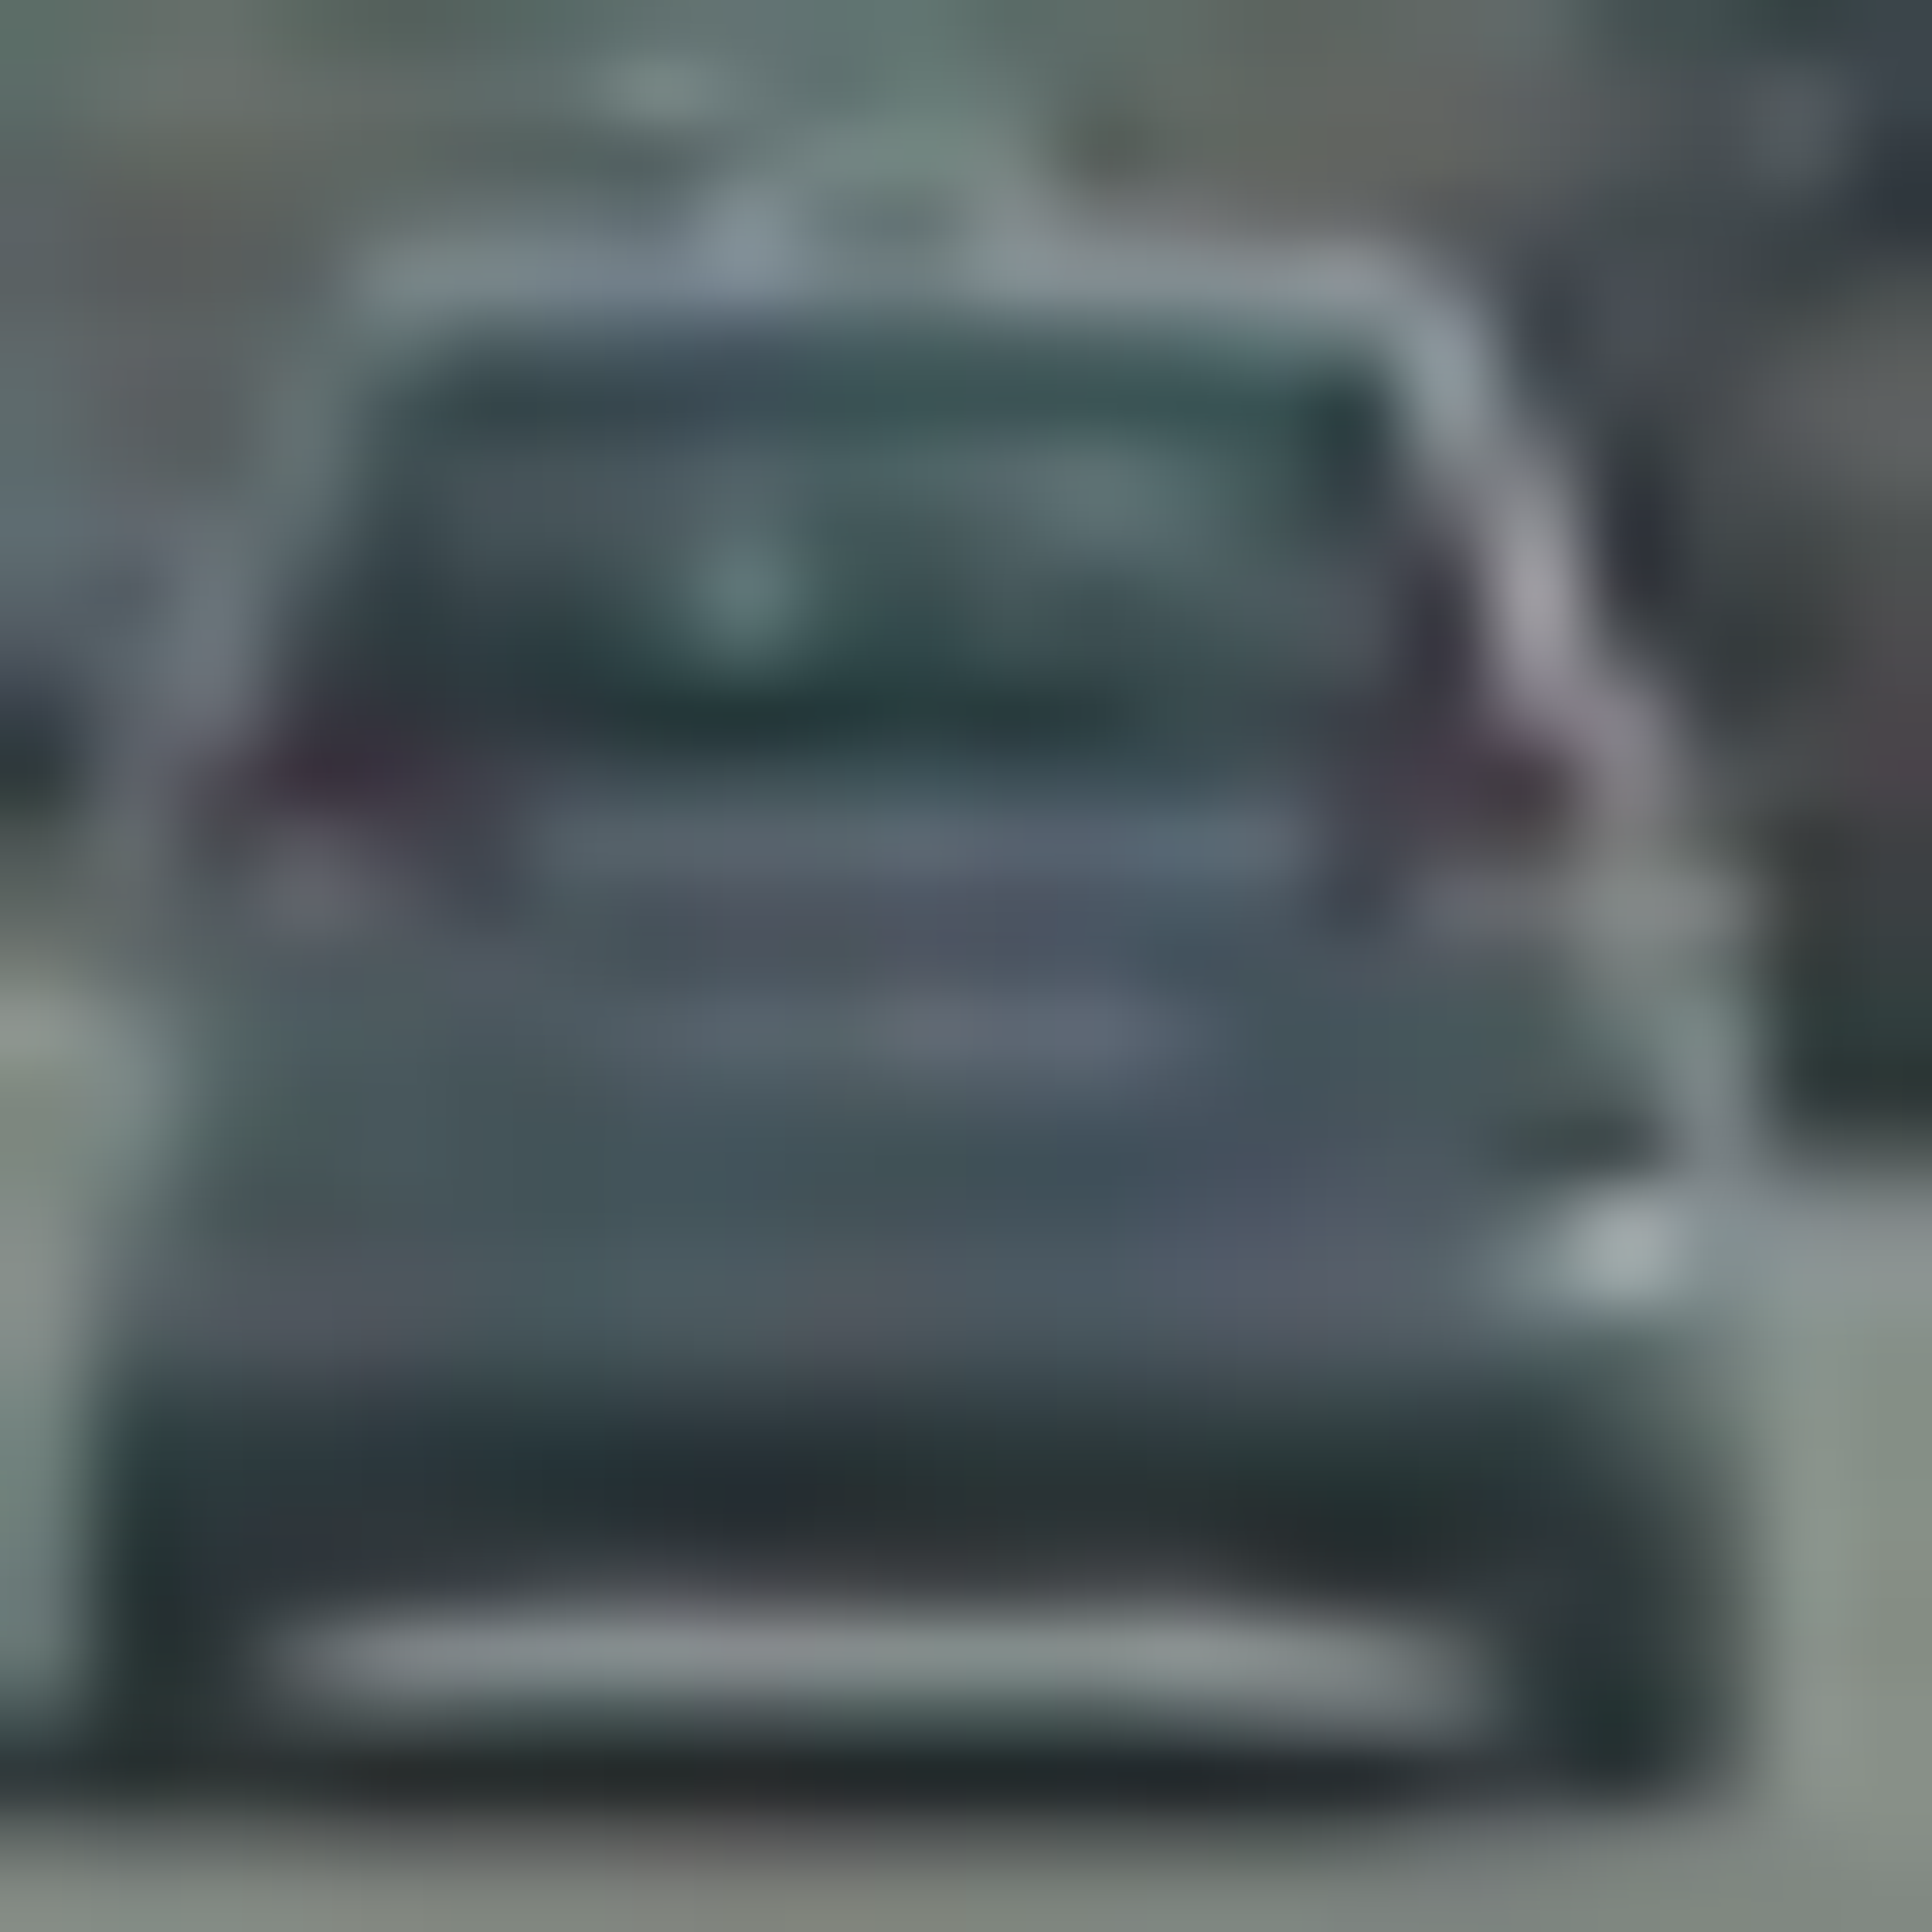
\includegraphics[width = 7cm]{images/DatasetGTILatihMobilJauh}}
			\subfloat[ ]{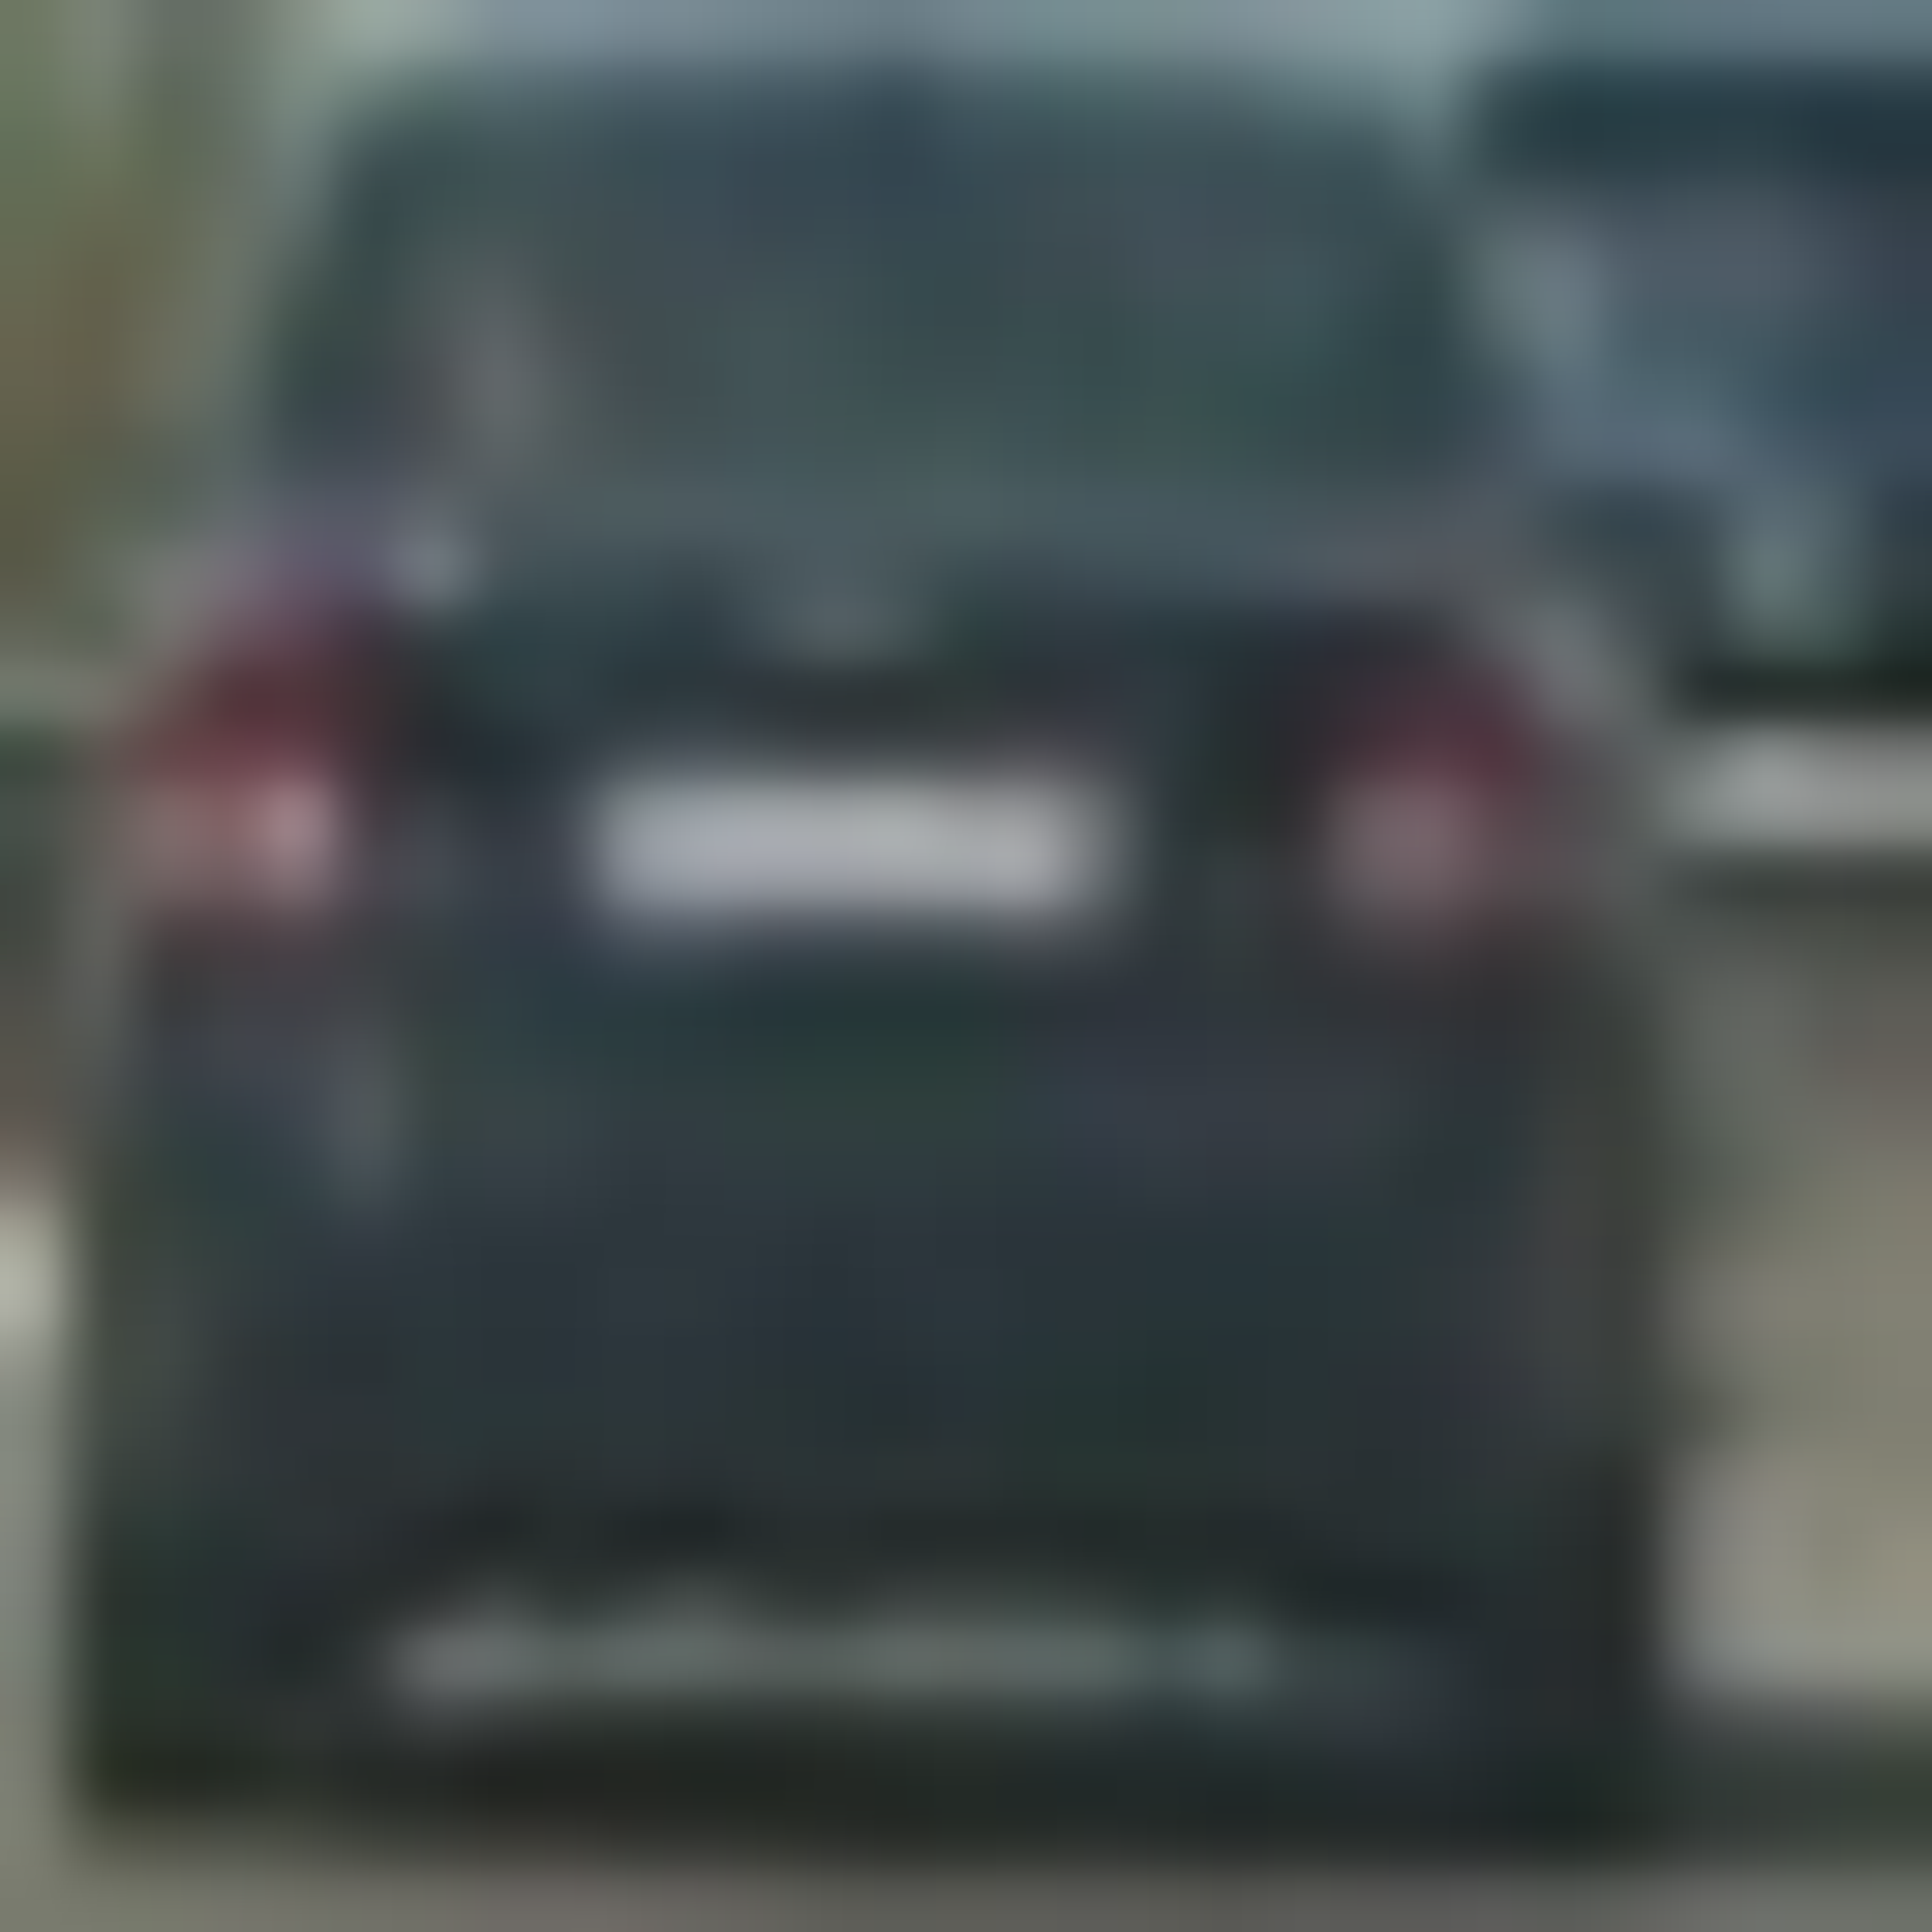
\includegraphics[width = 7cm]{images/DatasetGTILatihMobilDekat}}\\
			\subfloat[ ]{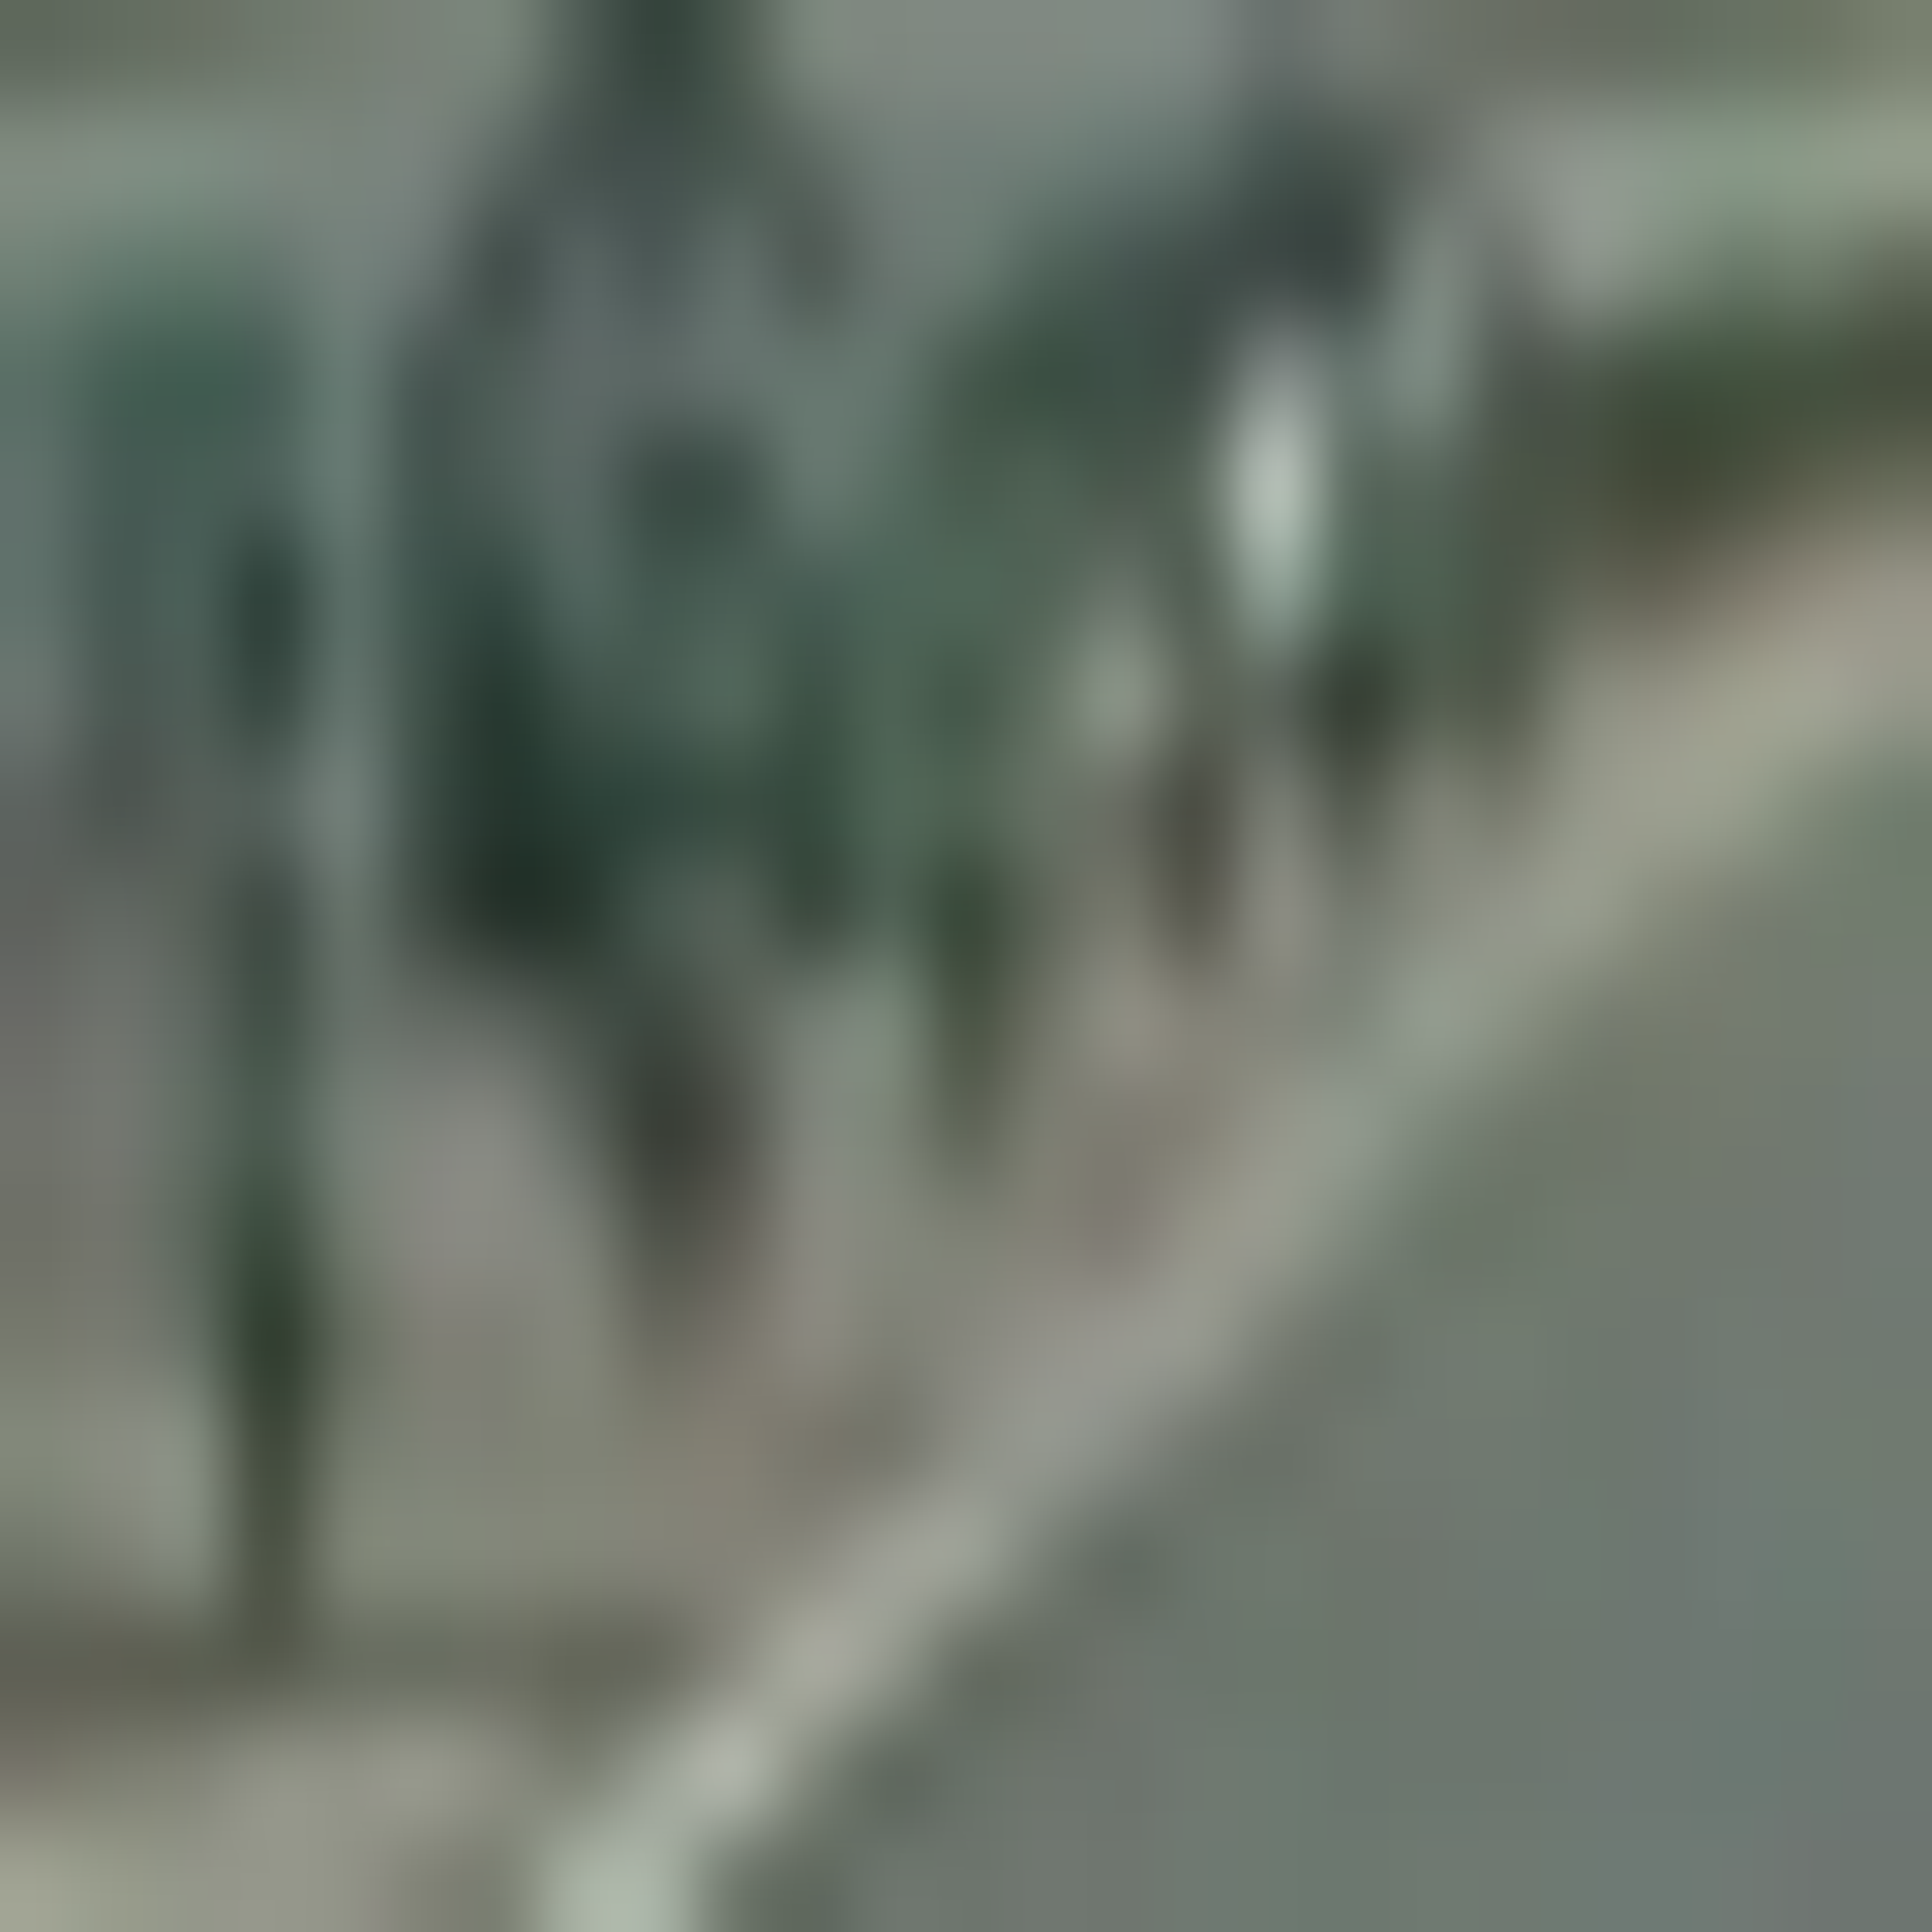
\includegraphics[width = 7cm]{images/DatasetGTILatihBukanMobil}}
			\subfloat[ ]{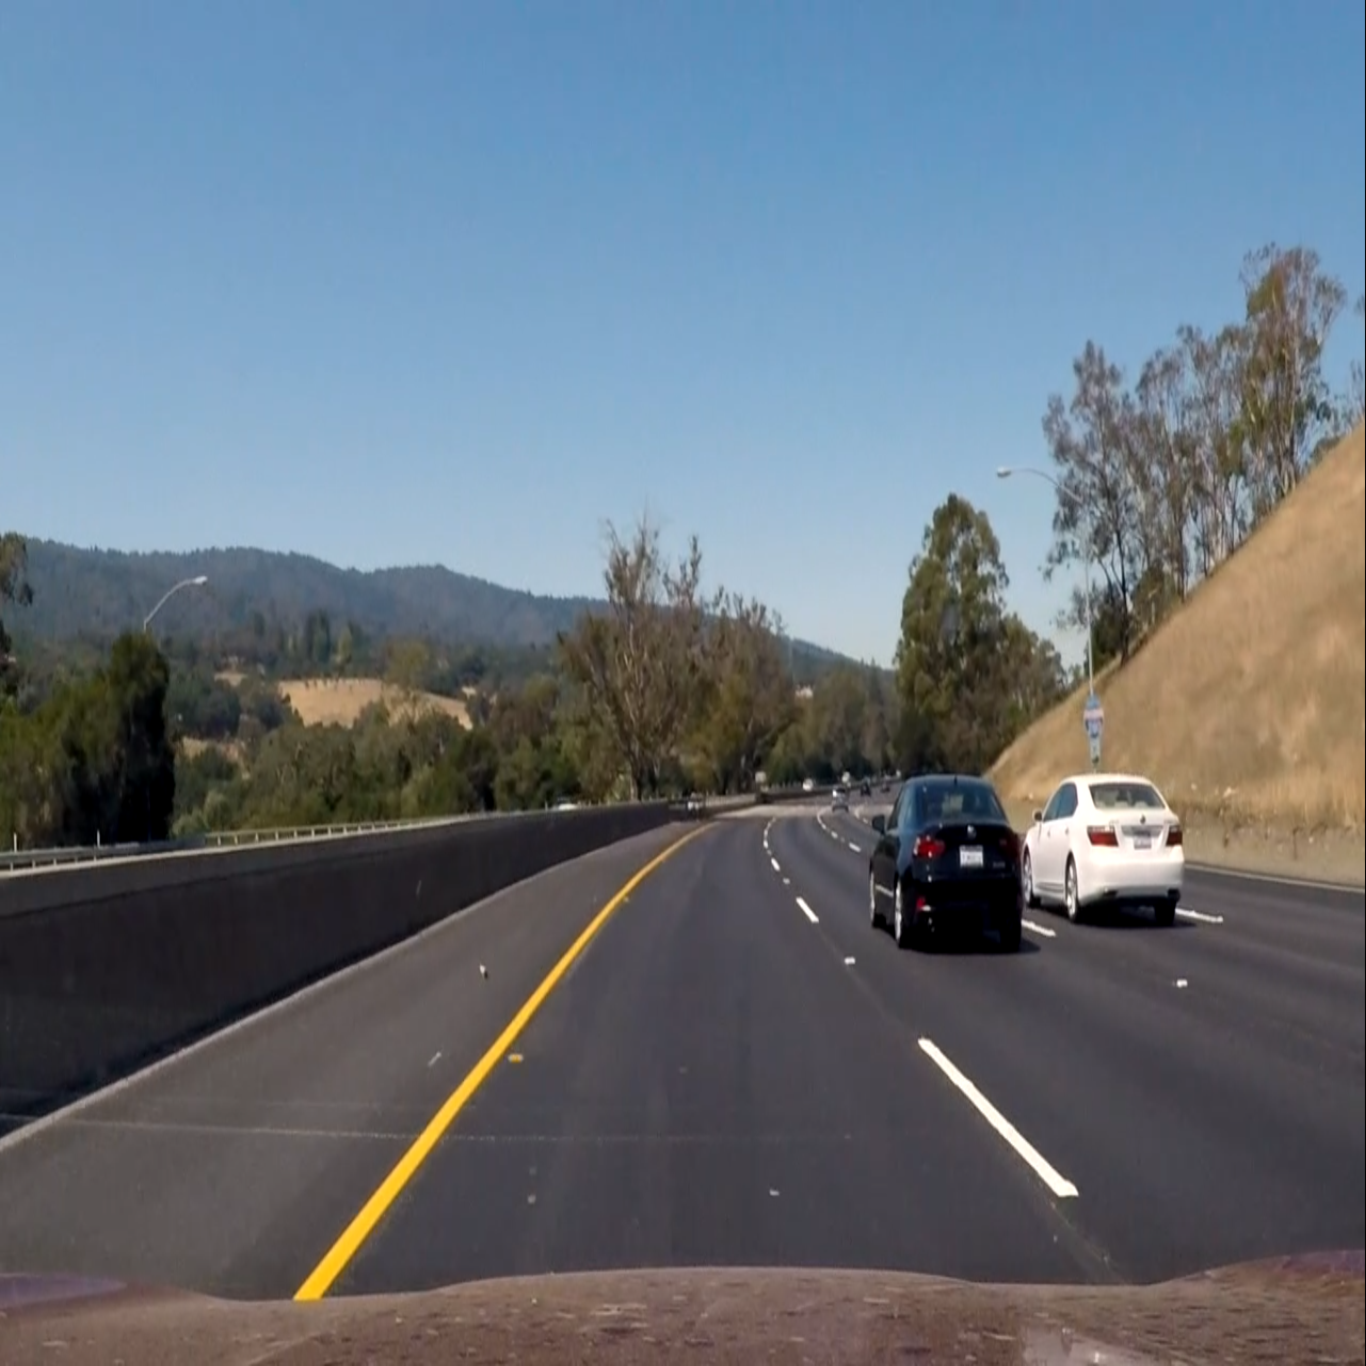
\includegraphics[width = 7cm]{images/DatasetGTIUji}}\\
		\end{figure} \\
			\hline
		\end{tabular}
	\end{adjustbox}
	\captionof{figure}{Contoh \textit{Dataset GTI}. (a) Data Latih Mobil (kiri) (b) Data Latih Mobil (kanan) (c) Data Latih Mobil (jauh) (d) Data Latih Mobil (dekat) (e) Data Latih Bukan Mobil (f) Data Uji}
	\label{fig:ContohGTI}
\end{table}

\textit{Dataset KITTI Database} diperoleh dari \textit{http://www.cvlibs.net/datasets/kitti/}. \textit{Dataset KITTI} merupkan data latih yang berupa mobil yang sama dengan GTI, namun dengan kondisi pencahayaan dan arah yang berbeda. Citra yang diambil dari \textit{dataset} merupakan citra RGB dengan 24 channel warna. Untuk proses pelatihan, ada total 5966 data citra yang diambil dari \textit{dataset}.

\begin{table}[H]
	\small
	\begin{adjustbox}{width=1\textwidth}
		\begin{tabular}{| p {14cm} |}
			\hline
			\begin{figure}[H]
				\centering
				{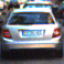
\includegraphics[width = 5cm]{images/DatasetKITTILatihMobil}}
				{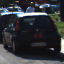
\includegraphics[width = 5cm]{images/DatasetKITTILatihMobil1}}
				{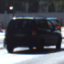
\includegraphics[width = 5cm]{images/DatasetKITTILatihMobil2}}
			\end{figure} \\
			\hline
		\end{tabular}
	\end{adjustbox}
	\captionof{figure}{Contoh \textit{Dataset KITTI}, data data latih mobil}
	\label{fig:ContohKITTI}
\end{table}

Ukuran setiap data latih akan diubah menjadi berukuran 64 x 64 piksel. Format citra dari \textit{dataset} ini akan diubah \textit{Portable Gray Map} (PGM) dengan 8 bit kedalaman \textit{depth}. Data latih dibagi menjadi 2 jenis yaitu mobil (kondisi utuh, tidak ada bagian mobil yang terpotong) dan bukan mobil (jalanan, motor, rumah, pejalan kaki, dan sebagainya). Pembagian data latih terdiri dari 4 jenis pengambilan citra, yaitu jauh, dekat, kiri, dan kanan.

Untuk citra uji, terdiri dari mobil yang berbeda - beda. Citra data uji diambil dari \textit{www.youtube.com} yang akan diproses secara citra digital. Dari video akan diambil beberapa frame untuk dideteksi keberadaan mobil. Ukuran untuk setiap citra uji beragam dengan panjang antara 110 piksel sampai 301 piksel dan lebar 75 piksel sampai 179 piksel dengan \textit{depth bit} 24.

Pada dataset juga terdapat \textit{template} untuk \textit{Region of Interest} dimana berupa citra biner yang berfungsi untuk menandai lokasi dimana mobil akan melaju. ROI digunakan pada saat proses \textit{testing}. Penggunaan ROI ditandai dengan nilai 1 untuk \textit{foreground} dan 0 untuk \textit{background}.

\begin{table}[H]
	\small
	\begin{adjustbox}{width=1\textwidth}
		\begin{tabular}{| p {14cm} |}
			\hline
			\begin{figure}[H]
				\centering
				{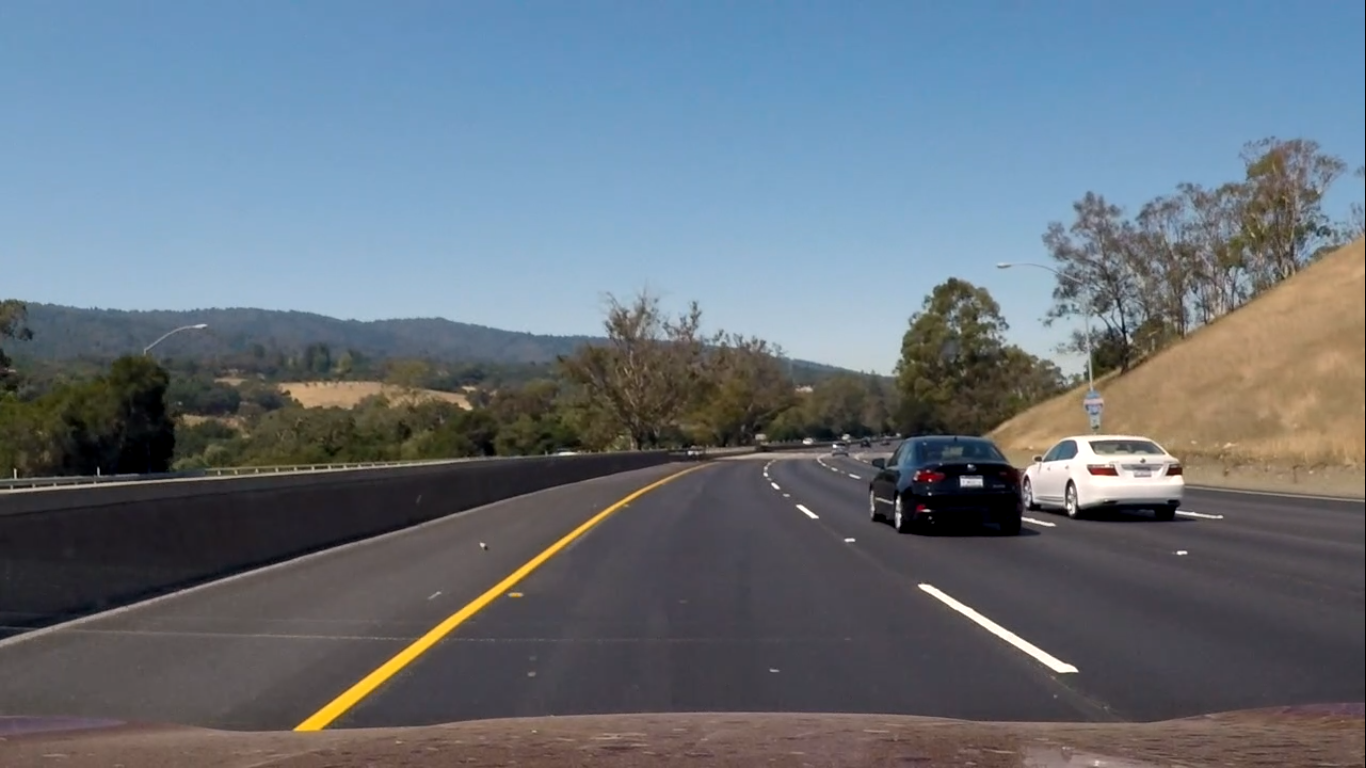
\includegraphics[height = 4cm]{images/ROI}} 
				{
\includegraphics[height = 4cm]{images/ROI_biner}}\\
			\end{figure} \\
			\hline
		\end{tabular}
	\end{adjustbox}
	\captionof{figure}{Contoh ROI}
	\label{fig:ContohROI}
\end{table}

Analisis selanjutnya akan dilakukan untuk menangani kasus dimana bagian dari mobil yang terdapat dalam citra uji hanya sebagian, terdapat lebih dari 1 mobil dalam 1 citra uji, dan ukuran objek berdasar jarak kamera dengan objek penelitian (mobil). Mobil yang akan terdeteksi memiliki ukuran terkecil 64 x 64 piksel.
\\

\subsection{Tahap Pendeteksian Lokasi Mobil}
Seperti dijelaskan sebelumnya, sistem pendeteksian mobil terdiri dari beberapa tahap. Citra input pertama - tama dibuat menjadi \textit{grayscale}, kemudian melalui tahap ekstraksi fitur dengan \textit{Histogram of Oriented Gradients}, dan terakhir fitur yang diperoleh kemudian diklasifikasi dengan \textit{Support Vector Machines}. Berikut adalah skema alur dari tahap pendeteksian lokasi mobil.
\\

\subsubsection{\textit{Grayscale}}
Proses pertama yaitu mengubah citra masukan menjadi citra \textit{grayscale}. Tujuan dari \textit{grayscaling} citra adalah untuk menghilangkan informasi warna dari setiap piksel citra. Dalam proses deteksi mobil dengan HOG, input warna tidak diperlukan karena warna tidak diperlukan oleh metode HOG. Di bawah merupakan contoh matriks citra asli dengan 3 \textit{channel} warna yaitu \textit{Red}, \textit{Green}, dan \textit{Blue} berukuran 5 $\times$ 5 piksel yang diambil dengan menggunakan \textit{image tools} dari aplikasi \textit{MatLab}. \\

\begin{adjustbox}{width=1\textwidth}
	\begin{minipage}{\linewidth}
		\framebox[\textwidth]{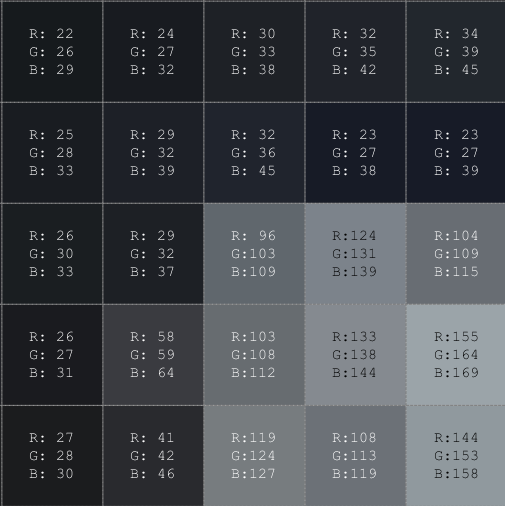
\includegraphics[width=5cm]{images/CitraMatriksAsal.PNG}}
		\captionof{figure}{Matriks Citra Asal berukuran 5 $\times$ 5\\}
		\label{fig:MatriksCitraAsal}
	\end{minipage}
\end{adjustbox} \\

Dari contoh nilai citra RGB di atas, akan diubah menjadi nilai \textit{grayscale} menggunakan rumus \eqref{eq:grayscale} dengan perhitungan sebagai berikut:

\begin{table}[H]
	\begin{adjustbox}{width=1\textwidth}
		\begin{tabular}{|p{13.55cm}|}
			\hline
			\begin{equation}\nonumber
			\begin{aligned}
			Matriks[3,3] &= (0.299 * 133) + (0.587 * 138) + (0.114 * 144) \\
						 &= 137.189 \approx 137 
			\end{aligned}
			\end{equation}\\
			\hline
		\end{tabular}
	\end{adjustbox}
\end{table}

Perhitungan di atas diterapkan pada seluruh piksel pada citra asal yang kemudian menghasilkan matriks citra berukuran 5 $\times$ 5 dengan satu nilai derajat keabuan.

\begin{adjustbox}{width=1\textwidth}
	\noindent\begin{minipage}{\linewidth}
		\framebox[\textwidth]{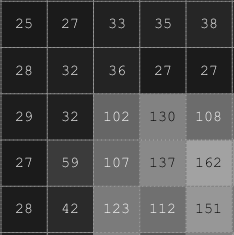
\includegraphics[width=5cm]{images/CitraMatriksGrayscale.PNG}}
		\captionof{figure}{Matriks Citra Hasil Grayscale\\}
		\label{fig:MatriksCitraGrayscale}
	\end{minipage}
\end{adjustbox} \\

\subsection{\textit{Histogram of Oriented Gradient}}
Hasil citra \textit{grayscale} dari \textit{preprocessing} kemudian digunakan untuk input HOG. HOG bertujuan untuk mengambil fitur dari citra masukkan. Hasil dari proses ini adalah vektor fitur yang berbentuk matriks fitur dimana ukurannya ditentukan berdasar jumlah \textit{bin}, ukuran sel dan blok. Ukuran sel, blok, dan jumlah \textit{bin} akan dianalisis pada bab selanjutnya.
%Metode HOG pada penelitian ini dijelaskan melalui \textit{pseudocode} berikut:

\noindent\fbox{\parbox{\textwidth}{\textit{Peseudocode:}
\begin{enumerate}
	\item \textbf{Masukan:} Citra \textit{grayscale} hasil resize.
	\item Menentukan jumlah \textit{bin}, ukuran sel, dan ukuran blok.
	\item Menghitung nilai gradien dan arah gradien untuk setiap piksel dari citra masukan dengan persamaan \ref{eqn:BesarGradien} dan \ref{eqn:ArahGradien}.
	\item Menghitung nilai magnitude gradien dan arah gradien untuk setiap piksel dari citra masukan menggunakan hasil dari tahap 2 sebelumnya.
	\item Membagi citra masukan ke dalam ukuran sel yang sudah ditentukan.
	\item Untuk setiap sel, lakukan proses vote untuk setiap c \textit{bin} terhadap sudutnya dengan menggunakan magnitude gradien dan arah gradien dari tahap 4.
	\item Untuk setiap blok (a x b sel), gabungkan histogram \textit{bin} ke dalam satu matriks baris, sehingga didapat ukuran [a x b x c] x 1 matriks untuk proses normalisasi.
	\item Menggunakan rumus algoritme \textit{L2 Norm} dengan menggunakan persamaan \ref{eqn:normalisasi2} dalam proses normalisasi kemudian lakukan proses normalisasi berupa \textit{sliding window} dengan melakukan pergeseran sebesar ukuran 1 sel ke arah vertikal dan horizontal dari hasil tahap 6.
	\item Untuk setiap hasil normalisasi, gabungkan seluruh matriks baris sehingga membentuk sebuah fitur yang besar dengan ukuran (jumlah pergeseran vertikal) x (jumlah pergeserah horizontal) x (a x b x c).
	\item \textbf{Keluaran:} Vektor Fitur dari tahap normalisasi.
\end{enumerate}}}

Berdasarkan \textit{pseudocode} di atas, akan dilakukan langkah - langkah untuk menghitung matriks fitur vektor. Berdasarkan penelitian \cite{dalal}, ukuran sel yang digunakan adalah 8 x 8 piksel. Ukuran sel akan mempengaruhi jumlah fitur. Semakin kecil jumlah sel, maka jumlah fitur akan bertambah. Pada proses \textit{Histogram of Oriented Gradients}, contoh masukan untuk proses ini berupa citra \textit{grayscale} yang sudah diproses melalui \textit{resize} citra menjadi ukuran 4 $\times$ 4 piksel.

\begin{table}[H]
	\centering
	\begin{small}
		\begin{tabular}{|p{2cm}|p{2cm}|p{2cm}|p{2cm}|}
			\hline
			89 & 92 & 88 & 92 \\
			\hline
			90 & 88 & 90 & 86 \\
			\hline
			91 & 90 & 90 & 94 \\
			\hline
			91 & 122 & 91 & 122 \\
			\hline
		\end{tabular}
	\end{small}
	\captionof{figure}{Contoh sebagian matriks citra hasil \textit{preprocessing} dalam ukuran 4 x 4 piksel\\}
	\label{fig:MatriksCitraHasilPreprocessing}
\end{table}

Langkah pertama adalah menghitung nilai gradien dari posisi vertikal dan horizontal untuk setiap piksel menggunakan persamaan \eqref{eqn:GradientH} dan \eqref{eqn:GradientV}.

\begin{equation*}
	G_{x}(2,5) = 89 - 89 = 0
\end{equation*}
\begin{equation*}
	G_{y}(2,5) = 85 - 122 = -37
\end{equation*}

Langkah pertama diterapkan untuk seluruh piksel pada citra. Berikut contoh dari visualisasi fitur HOG.

\begin{table}[H]
	\small
	\begin{adjustbox}{width=1\textwidth}
		\begin{tabular}{| p {14cm} |}
			\hline
			\begin{figure}[H]
				\centering
				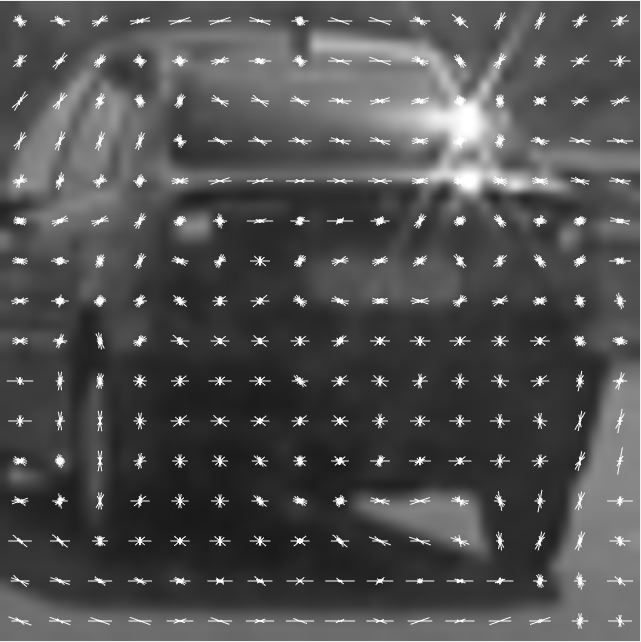
\includegraphics[width=7cm]{images/car_hog_gray4x4}
			\end{figure} \\
			\hline
		\end{tabular}
	\end{adjustbox}
	\captionof{figure}{Visualisasi Fitur HOG dengan ukuran sel 4 x 4 piksel}
	\label{fig:FiturHOG}
\end{table}

Untuk setiap piksel, hitung \textit{magnitude} gradien menggunakan persamaan \eqref{eqn:BesarGradien} dan arah gradien menggunakan persamaan \eqref{eqn:ArahGradien}.

\begin{equation*}
M(2,5) = \sqrt{0^2 + (-37)^2} = 37
\end{equation*}
\begin{equation*}
\theta(2,5) = arctan\frac{-37}{0} = 90
\end{equation*}

Setelah itu, tentukan ukuran sel, ukuran blok dan jumlah \textit{bins}. Pada awalnya, ukuran sel akan dipilih sebesar 2 $\times$ 2 piksel dan ukuran blok sebesar 2 kali lipat daripada ukuran sel yaitu 4 $\times$ 4 piksel. Lakukan perhitungan \textit{Histogram of Oriented Gradient} untuk semua sel dengan melakukan \textit{voting} arah gradien berdasarkan  \textit{magnitude} gradien, dimana arah gradien akan menjadi jumlah sudut \textit{bin}, dan \textit{magnitude} gradien akan menjadi bobot nilai yang kemudian dimasukkan berdasarkan persentase. Untuk contoh perhitungan analisis kali ini jumlah \textit{bins} yang dipakai sebanyak 9 buah, sehingga didapat nilai sudut setiap \textit{histogram bin} yaitu 180 / 4 = 45. Berikut merupakan contoh proses \textit{voting} untuk piksel dengan koordinat (2,5).

\begin{equation*}
M(2,5) = 37
\end{equation*}
\begin{equation*}
\theta(2,5) = 90
\end{equation*}

Sehingga untuk \textit{bin} dengan sudut 90 akan mendapat nilai bobot sebesar 37 yang didapatkan dari nilai gradien \textit{magnitude}-nya. Lakukan proses tersebut untuk setiap sel sampai setiap sel akan mempunyai \textit{Histogram of Oriented Gradient}. Kemudian untuk setiap blok akan dilakukan normalisasi dengan menggabungkan hasil histogram dari setiap sel dalam bloknya. Adapun proses normalisasi dapat menggunakan 4 algoritme yaitu, \textit{L1-Norm}, \textit{L1-Sqrt}, \textit{L2-Norm}, dan \textit{L2-Hys}. Penelitian ini akan menggunakan algoritme normalisasi \textit{L2-Norm} karena berdasarkan penelitian sebelumnya, hasil yang didapat lebih baik dari algoritme lainnya \cite{prahara}. Di bawah adalah contoh perhitungan normalisasi untuk blok pertama:
\begin{table}[H]
	\centering
	\begin{small}
		\begin{tabular}{|p{1cm}|p{1cm}|p{1cm}|p{1cm}|p{1cm}|p{1cm}|p{1cm}|p{1cm}|}
			\hline
			1 & 0 & 4 & 0 \\
			\hline
			0 & 0.76 & 36.24 & 0 \\
			\hline
			0 & 0 & 40 & 0 \\
			\hline
			0 & 1.65 & 36.35 & 0 \\
			\hline
		\end{tabular}
	\end{small}
	\captionof{figure}{Matriks hasil Perhitungan Histogram untuk seluruh sel\\}
	\label{fig:MatriksHasilPerhitunganHistogram}
\end{table}

Berdasarkan matriks pada gambar \ref{fig:MatriksHasilPerhitunganHistogram}. Elemen matriks yang akan kita gunakan dalam perhitungan normalisasi ini adalah seluruh elemen baris pertama dan baris kedua.

\begin{equation*}
L2_{Norm} = \sqrt{1^2 + 0^2 + 4^2 + 0^2 + \ldots + 36.5^2 + 0^2} = 51,360978379
\end{equation*}

Setiap nilai pada histogram dari sel dalam blok tersebut akan dibagi dengan nilai hasil normalisasinya. Berikut merupakan contoh matriks hasil perhitungan histogram baris pertama kolom 1-4.
\begin{gather*}
\begin{bmatrix}
0,019470034 & 0 & 0,077880136 & 0 \\
\end{bmatrix}
\end{gather*}

Lakukan proses normalisasi untuk setiap blok dengan menggeser secara horizontal sejauh 1 kali ukuran sel (setengah ukuran blok) dan kemudian secara vertikal sejauh 1 kali ukuran sel sa mpai blok tersebut sudah berada pada akhir dari bagian citra. Kemudian hasil dari proses normalisasi akan disusun menjadi matriks dengan kolom sebesar  \textit{jumlah bin} $\times$ \textit{lebar blok dalam satuan sel} $\times$ \textit{jumlah pergeseran horizontal} dan jumlah baris sebesar \textit{jumlah pergeseran vertikal} $\times$ \textit{tinggi blok dalam satuan sel} , dengan perhitungan tersebut, dalam analisa saat ini didapatkan ukuran matriks sebesar 6 $\times$ 8. Dalam analisa ini, hasil keluaran dari metode \textit{Histogram of Oriented Gradient} ada sebanyak 48 fitur. Matriks inilah yang akan dijadikan sebagai masukan bagi metode \textit{Machine Learning} yang akan digunakan dalam penelitian ini.\\

\subsection{\textit{Support Vector Machine}}
\textit{HOG descriptor} yang dihasilkan dari perhitungan metode \textit{Histogram of Oriented Gradient} akan digunakan sebagai bahan masukan \textit{Support Vector Machine}. Masukkan untuk metode SVM ini berupa matriks fitur berukuran jumlah data x jumlah data. \textit{Support Vector Machine} yang akan digunakan dalam penelitian ini akan menggunakan \textit{library} dari Weka SVM. \textit{Support Vector Machine} termasuk dalam algoritme \textit{supervised learning}. Konsep dasar dari metode ini adalah untuk menemukan sebuah \textit{separating hyperplane} (bidang) yang dapat memisahkan dua kelas sebagai keputusan klasifikasi. Dalam penelitian ini mobil yang akan dikenali adalah semua jenis mobil dari arah kiri dan kanan.

\begin{small}
	\begin{longtable}{| p {0.75cm} | p {0.7cm} | p {0.7cm} | p {0.7cm} | p {0.7cm} | p {0.7cm} | p {0.7cm} |  p {0.7cm} | p {0.7cm} | p {0.7cm} | p {0.7cm} | p {0.7cm} | p {0.7cm} | p {0.7cm} |}
		\caption{Tabel Contoh Data Latih} \\
		\hline
		\textbf{Data}  & \textbf{f1}  & \textbf{f2}  & \textbf{f3} & \textbf{f4} & \textbf{Class} \\
		\hline
		\endfirsthead
		\endhead
		\textbf{A1} & 5.1 & 3.5 & 1.4 & 0.2 & 1\\
		\hline
		\textbf{A2} & 4.9 & 3.0 & 1.4 & 0.2 & 1\\
		\hline
		\textbf{A3} & 7.0 & 3.2 & 4.7 & 1.4 & -1\\
		\hline
		\textbf{A4} & 6.4 & 3.2 & 4.5 & 1.5 & -1\\
		\hline
	\end{longtable}
\end{small}

Pada matriks fitur di atas, 1 menandakan kelas mobil dan -1 menandakan kelas bukan mobil. Berdasarkan matriks fitur tersebut, akan dibuat matriks RBF dengan ukuran sebanyak data. Misal terdapat 4 data yang digunakan maka ukuran matriks RBF adalah $4\times4$. Matriks RBF digunakan untuk menghitung \textit{dot product} dari masing-masing data. Pada perhitungan ini nilai $\sigma$ yang digunakan adalah 1.\\
\\
K(A1,A1) = $\exp(-\frac{|A1-A1|^2}{2\sigma^2})$
$=\exp(-\frac{|5.1-5.1|^2+|3.5-3.5|^2+|1.4-1.4|^2
+|0.2-0.2|^2}{2(1)^2})$\\
$=1$
\\\\
K(A1,A2) = $\exp(-\frac{|A1-A2|^2}{2\sigma^2})$
$=\exp(-\frac{|5.1-4.9|^2+|3.5-3.0|^2+|1.4-1.4|^2
	+|0.2-0.2|^2}{2(1)^2})$\\
$=0.8650222931107414$
\\\\
K(A1,A3) = $\exp(-\frac{|A1-A3|^2}{2\sigma^2})$
$=\exp(-\frac{|5.1-7.0|^2+|3.5-3.2|^2+|1.4-4.7|^2
	+|0.2-1.4|^2}{2(1)^2})$\\
$=3.3046824003738314E^{-4}$
\\\\
K(A1,A4) = $\exp(-\frac{|A1-A4|^2}{2\sigma^2})$
$=\exp(-\frac{|5.1-6.4|^2+|3.5-3.2|^2+|1.4-4.5|^2
	+|0.2-1.5|^2}{2(1)^2})$\\
$=0.001444488499020542$
\\\\
Dari perhitungan \textit{dot product} di atas maka akan terbentuk matriks RBF seperti pada tabel 3.4.
\begin{small}
	\begin{longtable}{| p {2cm} | p {2cm} | p {2cm} | p {2cm} | p {2cm} |}
		\caption{Tabel Perhitungan Matriks RBF} \\
		\hline
		\textbf{}  & \textbf{A1}  & \textbf{A2}  & \textbf{A3} & \textbf{A4} \\
		\hline
		\endfirsthead
		\endhead	
		\textbf{A1}&1 & 0.865022293	& 3.30E-4 &	1.44E-03\\
		\hline
		\textbf{A2}& 0.865022293 & 1 & 2.27E-4 & 1.11E-03\\
		\hline
		\textbf{A3}& 3.30E-4 & 2.27E-4 & 1	& 0.814647316\\
		\hline
		\textbf{A4}& 1.44E-03 & 1.11E-03 & 0.814647316 & 1\\
		\hline
		\hline
		
	\end{longtable}
\end{small}

Setelah mendapatkan matriks RBF, maka dapat membuat persamaan linear untuk mendapatkan nilai $\alpha$ dan $b$ (bias) berdasarkan persamaan \textit{hyperplane} SVM yaitu persamaan \ref{eqn:rbfkernel}.\\
Contoh perhitungan:\\
$(1)\alpha_1 + (1)\alpha_2 + (-1)\alpha_3 + (-1)\alpha_4 + (0)b = 0$\\
$(1)\alpha_1 + (0.865022293)\alpha_2 + (-3.30E^{-4})\alpha_3 + (-1.44E^{-3})\alpha_4 + b = 1$\\
$(0.865022293)\alpha_1 + (1)\alpha_2 + (-2.27E^{-4})\alpha_3 + (-1.11E^{-3})\alpha_4 + b = 1$\\
$(3.30E^{-4})\alpha_1 + (2.27E^{-4})\alpha_2 + (-1)\alpha_3 + (-0.814647316)\alpha_4 + b = -1$\\
$(1.44E^{-3})\alpha_1 + (1.11E^{-3})\alpha_2 + (-0.814647316)\alpha_3 + (-1)\alpha_4 + b = -1$\\

Untuk mendapatkan solusi ($\alpha_1, \alpha_2, \alpha_3, \alpha_4, b$) dari sistem persamaan linear di atas dapat menggunakan \textit{library} JAMA. Berikut adalah solusi yang diperoleh dari sistem persamaan di atas.
\begin{small}
	\begin{longtable}{| p {2cm} | p {2cm} | p {2cm} | p {2cm} | p {2cm} |}
		\caption{Tabel nilai $\alpha$ dan $b$} \\
		\hline
		$\alpha_1$  & $\alpha_2$  & $\alpha_3$ & $\alpha_4$ & $b$ \\
		\hline
		\endfirsthead
		\endhead
		0.544855 & 0.543123 & 0.541044 & 0.546933 & -0.013700\\
		\hline
		
	\end{longtable}
\end{small}

Nilai $\alpha$ dan $b$ yang telah diperoleh kemudian disimpan untuk keperluan proses klasifikasi. Misal terdapat data uji sebagai berikut:
\begin{small}
	\begin{longtable}{| p {0.75cm} | p {0.7cm} | p {0.7cm} | p {0.7cm} | p {0.7cm} | p {0.7cm} | p {0.7cm} |  p {0.7cm} | p {0.7cm} | p {0.7cm} | p {0.7cm} | p {0.7cm} | p {0.7cm} | p {0.7cm} |}
		\caption{Tabel Contoh Data Uji} \\
		\hline
		\textbf{Data}  & \textbf{f1}  & \textbf{f2}  & \textbf{f3} & \textbf{f4} & \textbf{Class} \\
		\hline
		\endfirsthead
		\endhead
		\textbf{T1} & 4.6 & 3.1 & 1.5 & 0.2 & ?\\
		\hline
	\end{longtable}
\end{small}
Dalam proses pengujian, langkah yang ditempuh mirip dengan proses pelatihan. Pertama adalah membentuk matriks RBF untuk pengujian dengan menggunakan data latih pada tabel 3.3. Contoh perhitungan adalah sebagai berikut:\\\\
K(T1,A1) = $\exp(-\frac{|T1-A1|^2}{2\sigma^2})$
$=\exp(-\frac{|4.6-5.1|^2+|3.1-3.5|^2+|1.5-1.4|^2
	+|0.2-0.2|^2}{2(1)^2})$\\
$=0.8105842459701871$
\\\\
K(T1,A2) = $\exp(-\frac{|T1-A2|^2}{2\sigma^2})$
$=\exp(-\frac{|4.6-4.9|^2+|3.1-3.0|^2+|1.5-1.4|^2
	+|0.2-0.2|^2}{2(1)^2})$\\
$=0.9464851479534836$
\\\\
K(T1,A3) = $\exp(-\frac{|T1-A3|^2}{2\sigma^2})$
$=\exp(-\frac{|4.6-7.0|^2+|3.1-3.2|^2+|1.5-4.7|^2
	+|0.2-1.4|^2}{2(1)^2})$\\
$=1.6247279265951668E^{-4}$
\\\\
K(T1,A4) = $\exp(-\frac{|T1-A4|^2}{2\sigma^2})$
$=\exp(-\frac{|4.6-6.4|^2+|3.1-3.2|^2+|1.5-4.5|^2
	+|0.2-1.5|^2}{2(1)^2})$\\
$=9.396529058360945E^{-4}$
\\\\
Dari perhitungan \textit{dot product} maka akan terbentuk matriks RBF uji seperti pada tabel 3.7 di bawah ini.
\begin{small}
	\begin{longtable}{| p {2cm} | p {2cm} | p {2cm} | p {2cm} | p {2cm} |}
		\caption{Tabel Perhitungan Matriks RBF Uji} \\
		\hline
		\textbf{}  & \textbf{A1}  & \textbf{A2}  & \textbf{A3} & \textbf{A4} \\
		\hline
		\endfirsthead
		\endhead	
		\textbf{T1} & 0.810584245 & 0.946485147 & 1.62E-4 & 9.39E-4
		\\
		\hline	
	\end{longtable}
\end{small}
Setelah mendapatkan matriks RBF uji maka proses klasifikasi dapat dilakukan dengan menggunakan persamaan 2.15. Perhitungan klasifikasi adalah sebagai berikut:\\\\
$f(x) = sign[(0.810584 * 0.810584245  * 1.0) + (0.946485 * 0.946485147 * 1.0) + (1.624727 * 1.62E^{-4} * (-1.0)) + (9.396529 * 9.396529058E^{-4} * (-1.0)) + (-0.013700) ]$\\
$=1$

Setelah dilakukannya perhitungan manual antara data uji terhadap data latih, nilai yang diperoleh adalah 1 yang artinya data uji masuk ke dalam kelas 1 (positif). Jika hasil perhitungan bernilai -1 maka data uji masuk ke dalam kelas -1 (negatif). Misal dalam pengujian di atas kelas 1 adalah mobil dan kelas -1 adalah bukan mobil, maka data uji tergolong kelas mobil.
\newpage
%%-----------------------------------------------------------------------------%
\chapter{IMPLEMENTASI DAN PENGUJIAN}
%-----------------------------------------------------------------------------%

%
\vspace{4.5pt}
Pada bab ini akan menjelaskan mengenai proses implementasi dan pengujian terhadap sistem yang telah dibangun berdasarkan penjelasan pada bab sebelumnya.\\

\section{Lingkungan Implementasi}
Pada lingkungan implementasi, akan dijelaskan mengenai perangkat yang digunakan dalam proses pembangunan sistem baik dari perangkat keras maupun perangkat lunak yang digunakan.\\

\subsection{Spesifikasi Perangkat Keras}
Spesifikasi komputer yang digunakan dalam pembutan dan pengujian aplikasi deteksi bangunan pada citra udara dengan \textit{Convolutional Neural Network} adalah sebagai berikut:
\begin{enumerate}
	\item Komputer dengan \textit{processor} Intel Core i5-7400U CPU $@$ 2.70GHz
	\item \textit{Harddisk} dengan kapasitas 1 TB
	\item RAM 16 GB
	\item VGA NVDIA GeForce GT 1050M
	\\
\end{enumerate}

\subsection{Lingkungan Perangkat Lunak}
Spesifikasi perangkat lunak yang digunakan dalam pembangunan aplikasi deteksi bangunan pada citra udara dengan \textit{Convolutional Neural Network} adalah sebagai berikut:
7\begin{enumerate}
	\item \textit{Virtual Machine}: VMware Workstation 15
	\item Sistem Operasi: Ubuntu 18.04
	\item IDE: Geany 1.34.1
	\item Development Tool: Python 3.6.8 64-bit
	\\
\end{enumerate}

\section{Daftar Kelas dan Metode}
Pada bagian ini, akan dijelaskan mengenai \textit{class} dan \textit{method} yang digunakan dalam penelitian ini.
\\

\subsection{Daftar \textit{Class} dan \textit{Method} hog\_util\_functions}
Berikut adalah tabel berisi \textit{method} pada \textit{class} hog\_util\_functions. \textit{Class} hog\_util\_functions digunakan untuk mengolah citra menggunakan metode \textit{Histogram of Oriented Gradients}.

\begin{small}
	\begin{longtable}{|p{0.4cm}|p{2.6cm}|p{2cm}|p{2.5cm}|p{1.5cm}|p{4.5cm}|}
		\caption{Daftar Metode pada Kelas \textit{hog\_util\_functions}} \\	
		\hline
		\multirow{2}{*}{\textbf{No}} & \multirow{2}{*}{\textbf{Metode}} & \multicolumn{2}{c|}{\textit{\textbf{Input}}} & \multirow{2}{*}{\textit{\textbf{Output}}} & 
		\multirow{2}{*}{\textbf{Keterangan}}\\
		\cline{3-4}
		& & \textbf{Tipe} & \textbf{Variabel} & & \\
		\hline
		1 & convert\_rgb\_color & string \newline string & img \newline conv & image & Untuk mengubah \textit{color space}.\\
		\hline
		2 & get\_hog\_features & string \newline int \newline int \newline int \newline boolean \newline boolean & img \newline orient \newline pix\_per\_cell \newline cell\_per\_block \newline vis \newline feature\_vec & int[] & Untuk mengambil fitur menggunakan metode HOG.\\
		\hline
		3 & single\_image\_ \newline features & string \newline string \newline int[] \newline int \newline int \newline int \newline int \newline int \newline boolean \newline boolean \newline boolean & img \newline color\_space \newline spatial\_size \newline hist\_bins \newline orient \newline pix\_per\_cell \newline cell\_per\_block \newline hog\_channel \newline spatial\_feat \newline hist\_feat \newline hog\_feat & int[] & Untuk mengekstrak fitur dari satu jendela gambar.\\
		\hline
	\end{longtable}
\end{small}

\subsection{Daftar \textit{Class} dan \textit{Method} find\_cars}
Berikut adalah tabel berisi \textit{method} pada \textit{class} find\_cars. \textit{Class} find\_cars digunakan untuk mencari objek berupa mobil pada frame masukkan.
\begin{small}
	\begin{longtable}{|p{0.4cm}|p{2.6cm}|p{2cm}|p{2.5cm}|p{1.5cm}|p{4.5cm}|}
		\caption{Daftar Metode pada Kelas \textit{find\_cars}} \\	
		\hline
		\multirow{2}{*}{\textbf{No}} & \multirow{2}{*}{\textbf{Metode}} & \multicolumn{2}{c|}{\textit{\textbf{Input}}} & \multirow{2}{*}{\textit{\textbf{Output}}} & 
		\multirow{2}{*}{\textbf{Keterangan}}\\
		\cline{3-4}
		& & \textbf{Tipe} & \textbf{Variabel} & & \\
		\hline
		1 & load\_classifier & string & pickle\_file & int[] & Untuk memuat parameter HOG dan SVM dari \textit{pickle file}.\\
		\hline
		2 & draw\_labeled\_ \newline bboxes & string \newline string \newline int[][][] \newline int & img \newline labels \newline color \newline thick & image & Untuk membuat kotak penanda lokasi mobil yang terdeteksi.\\
		\hline
		3 & find\_cars & string \newline int \newline int \newline int \newline string \newline int \newline string[] \newline int & img \newline ystart \newline ystop \newline scale \newline svc \newline X\_scaler \newline params \newline cells\_per\_step & int[] & Untuk mengekstrak fitur menggunakan sub-sampling HOG dan membuat prediksi.\\
		\hline
	\end{longtable}
\end{small}

\subsection{Daftar \textit{Class} dan \textit{Method} train\_hog\_classifier}
Berikut adalah tabel berisi \textit{method} pada \textit{class} train\_hog\_classifier. \textit{Class} train\_hog\_classifier digunakan untuk proses pelatihan dari dataset.
\begin{small}
	\begin{longtable}{|p{0.4cm}|p{2.6cm}|p{2cm}|p{2.5cm}|p{1.5cm}|p{4.5cm}|}
		\caption{Daftar Metode pada Kelas \textit{train\_hog\_classifier}} \\	
		\hline
		\multirow{2}{*}{\textbf{No}} & \multirow{2}{*}{\textbf{Metode}} & \multicolumn{2}{c|}{\textit{\textbf{Input}}} & \multirow{2}{*}{\textit{\textbf{Output}}} & 
		\multirow{2}{*}{\textbf{Keterangan}}\\
		\cline{3-4}
		& & \textbf{Tipe} & \textbf{Variabel} & & \\
		\hline
		1 & load\_data\_sets &  &  & string[] \newline string[] & Untuk memuat data dari \textit{dataset}.\\
		\hline
		2 & save\_data\_sets & string \newline image[] \newline image[] & pickle\_file \newline cars \newline notcars &  & Untuk menyimpan daftar gambar mobil dan bukan mobil yang sudah dimuat.\\
		\hline
		3 & load\_cars\_norcars & string & data\_file & image[][] \newline image[][] & Untuk memuat \textit{dataset} dari \textit{pickle file}.\\
		\hline
		4 & save\_classifier\_ \newline data & string \newline int \newline int \newline int \newline int & pickle\_file \newline X\_train \newline Y\_train \newline X\_test \newline Y\_test &  & Untuk menyimpan dataset yang sudah dibagi menjadi data latih dan data uji.\\
		\hline
		5 & save\_classifier & string \newline string \newline int \newline string[] & pickle\_file \newline svc \newline X\_scaler \newline params \newline &  & Untuk menyimpan parameter HOG.\\
		\hline
		6 & extract\_features & image \newline string[] & imgs \newline params &  & Untuk mengekstrak fitur dari citra.\\
		\hline
	\end{longtable}
\end{small}

\section{Implementasi Perangkat Lunak}
Pada implementasi perangkat lunak dilakukan menurut analisis yang telah disusun
pada BAB III.\\

\subsection{Implementasi Pengambilan Dataset}
\textit{Dataset} GTI diperoleh dari \textit{http://www.gti.ssr.upm.es/data/Vehicle\_database.html} dan \textit{Dataset} KITTI dari \textit{http://www.cvlibs.net/datasets/kitti/}. Gambar \ref{img:FolderScheme} menunjukkan daftar \textit{folder} penyimpanan \textit{Dataset}.

\begin{table}[H]
	\small
	\begin{adjustbox}{width=1\textwidth}
		\begin{tabular}{| p {14cm} |}
			\hline
			\begin{figure}[H]
				\centering
				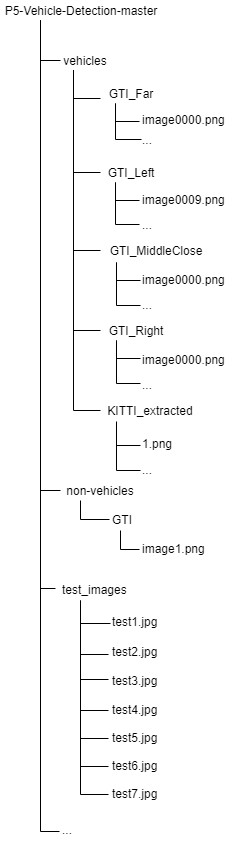
\includegraphics[width=7cm]{images/FolderScheme.png}
			\end{figure} \\
			\hline
		\end{tabular}
	\end{adjustbox}
	\captionof{figure}{Daftar folder \textit{Dataset}}
	\label{img:FolderScheme}
\end{table}  

Citra untuk proses pengenalan kendaraan terbagi menjadi 2 yaitu \textit{vehicles} dan \textit{non-vehicles}. Data citra \textit{vehicles} dibagi menjadi 5 macam yaitu \textit{GTI\_Far, GTI\_Left, GTI\_MiddleClose, GTI\_Right,} dan \textit{KITTI\_extracted}.
\textit{GTI\_Far} berisi citra yang diambil dari jauh. \textit{GTI\_Left} berisi citra yang diambil dari arah kiri kendaraan. \textit{GTI\_MiddleClose} berisi citra yang diambil dari dekat. \textit{GTI\_Right} berisi citra yang diambil dari arah kanan kendaraan. \textit{KITTI\_extracted} berisi citra yang terdiri dari variasi ukuran pengambilan citra. Hasil dari pengumpulan data akan disimpan dalam \textit{pickle file}. Untuk proses klasifikasi, citra dibagi 70\% untuk \textit{training} dan 30\% untuk \textit{testing}. Pembagian citra dilakukan secara acak.

Setelah proses pengenalan kendaraan selesai, hasil pengenalan kemudian digunakan untuk proses deteksi pada \textit{dataset} yang diambil dari \textit{http://www.youtube.com}. Dari \textit{dataset} yang berupa video, sudah terdapat 6 buah citra yang mewakili setiap kondisi pada folder \textit{test\_images}. Gambar \ref{fig:ContohDataDeteksi} menunjukkan citra untuk proses deteksi kendaraan.

\begin{table}[H]
	\small
	\begin{adjustbox}{width=1\textwidth}
		\begin{tabular}{| p {14cm} |}
			\hline
			\begin{figure}[H]
				\centering
				{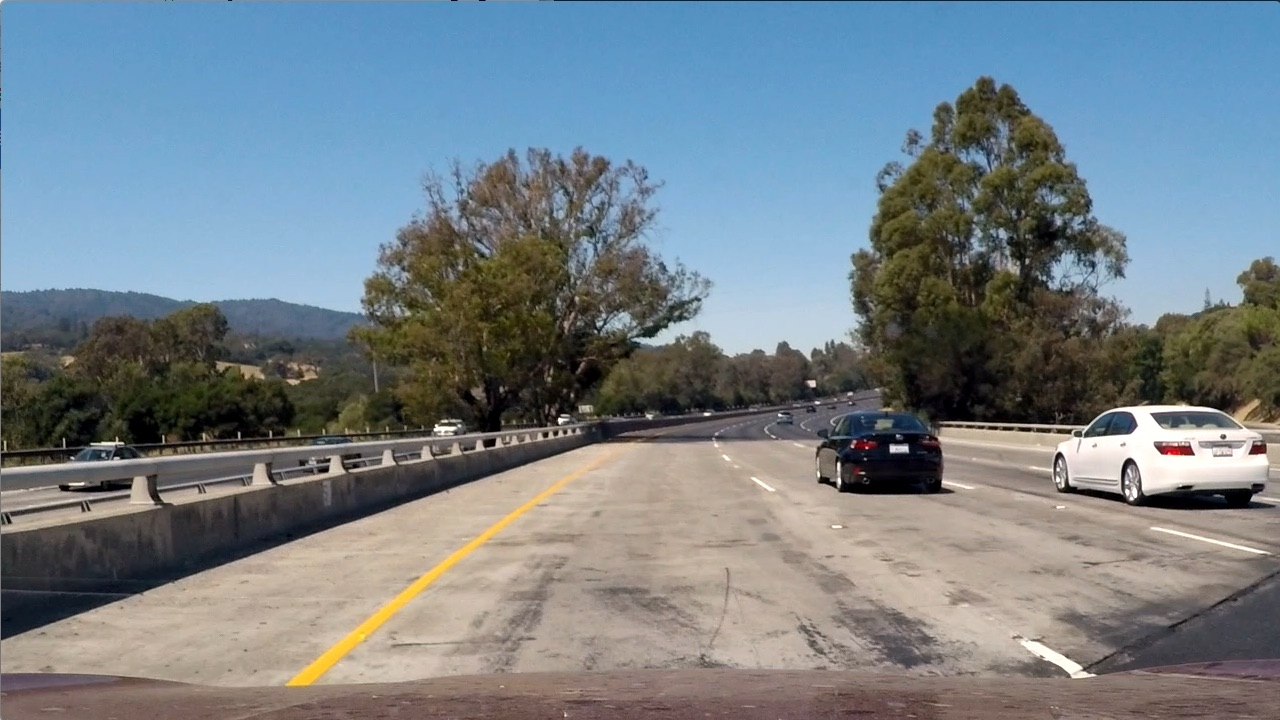
\includegraphics[width = 7cm]{images/test1}} 
				{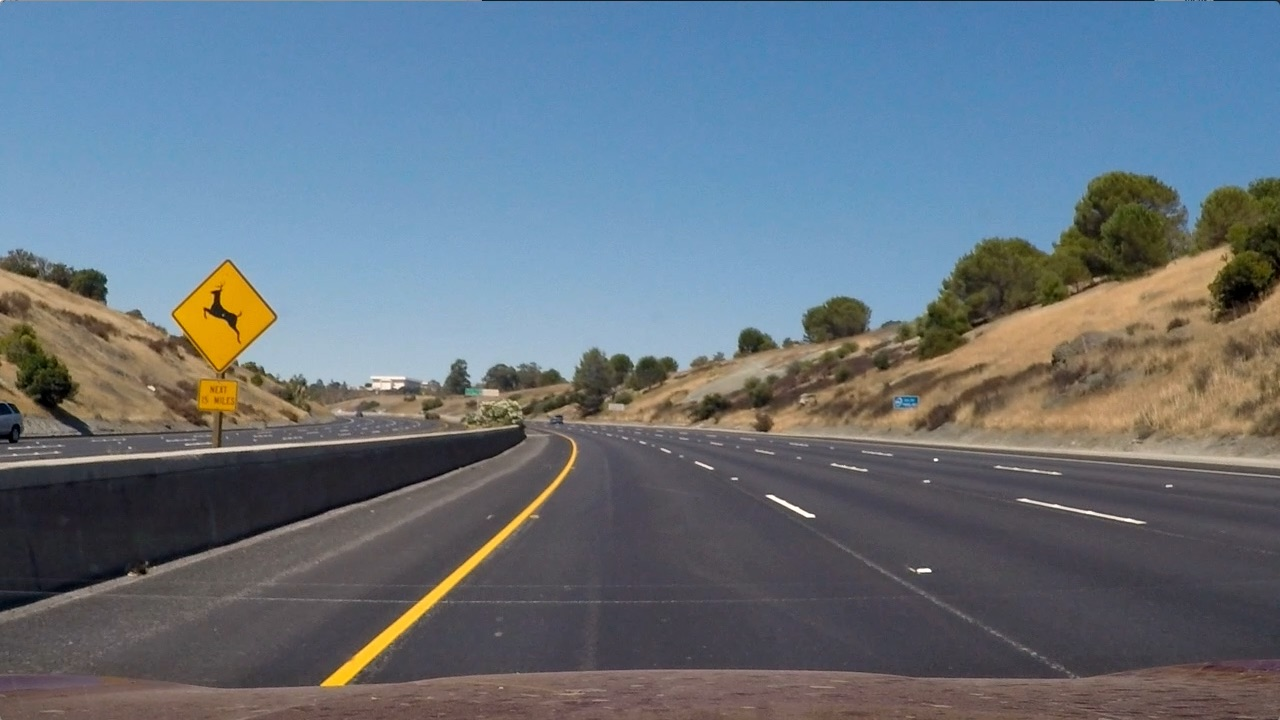
\includegraphics[width = 7cm]{images/test2}} \\
				{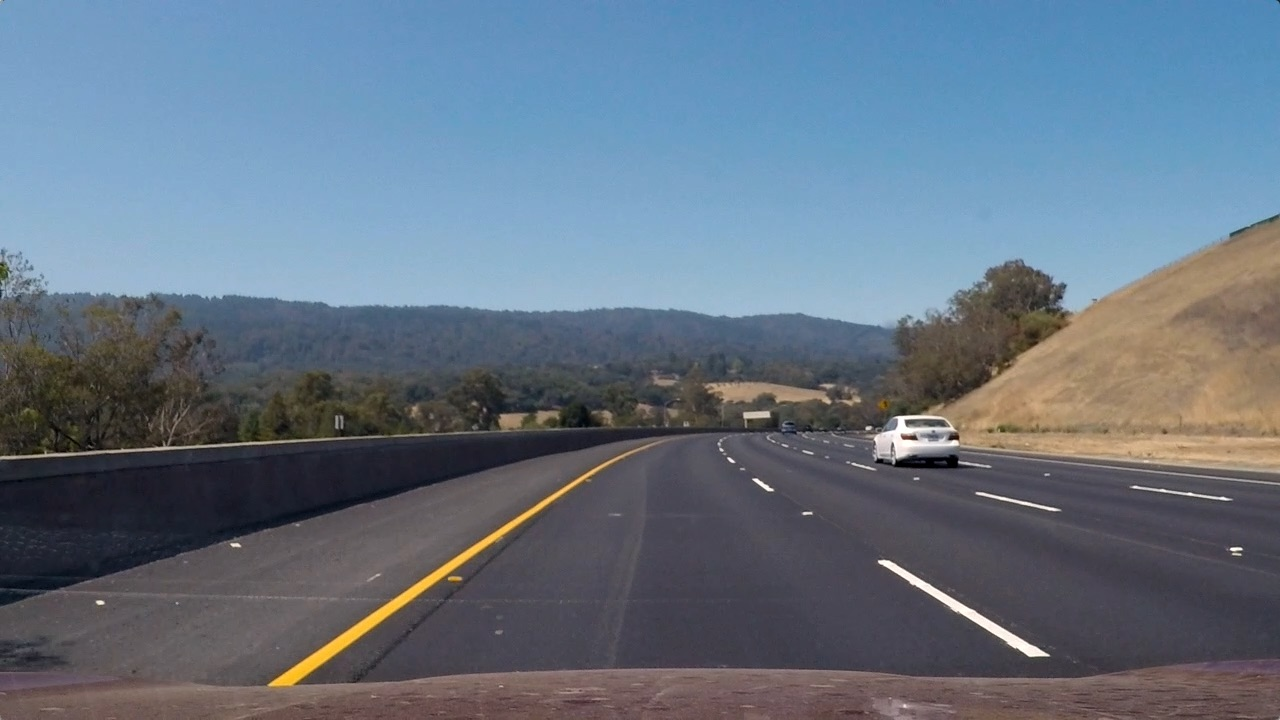
\includegraphics[width = 7cm]{images/test3}}
				{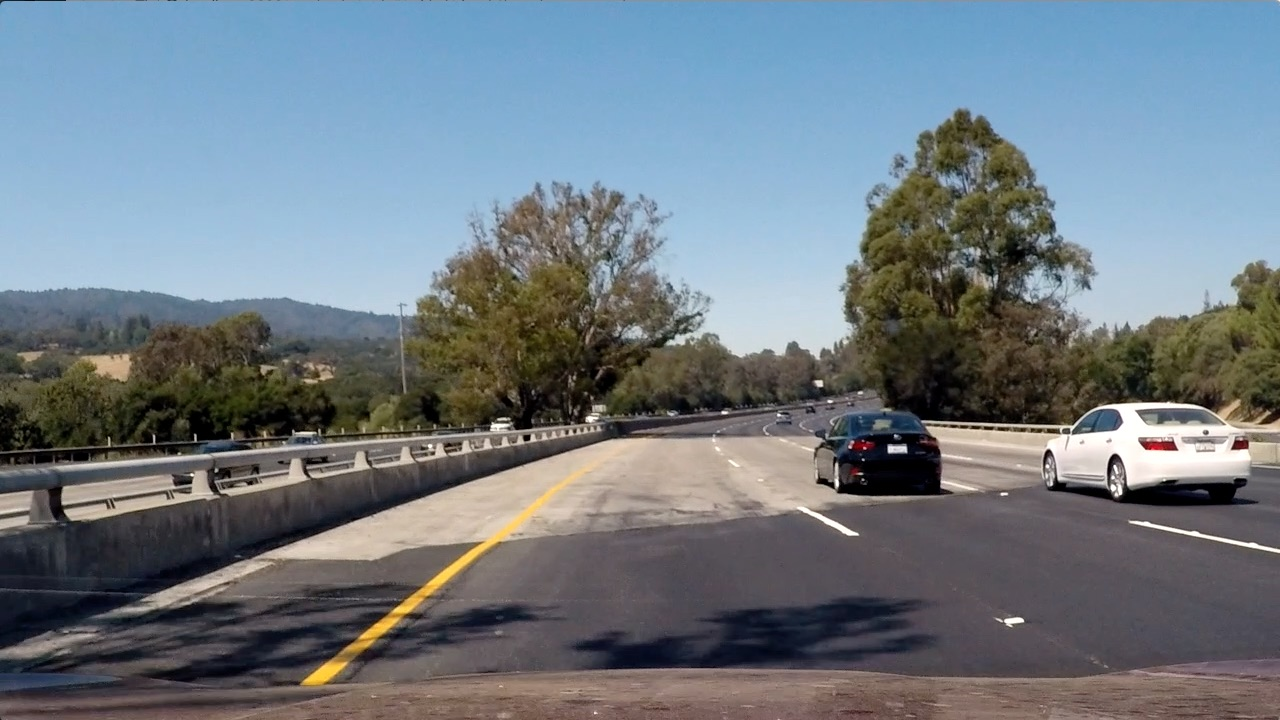
\includegraphics[width = 7cm]{images/test4}}\\
				{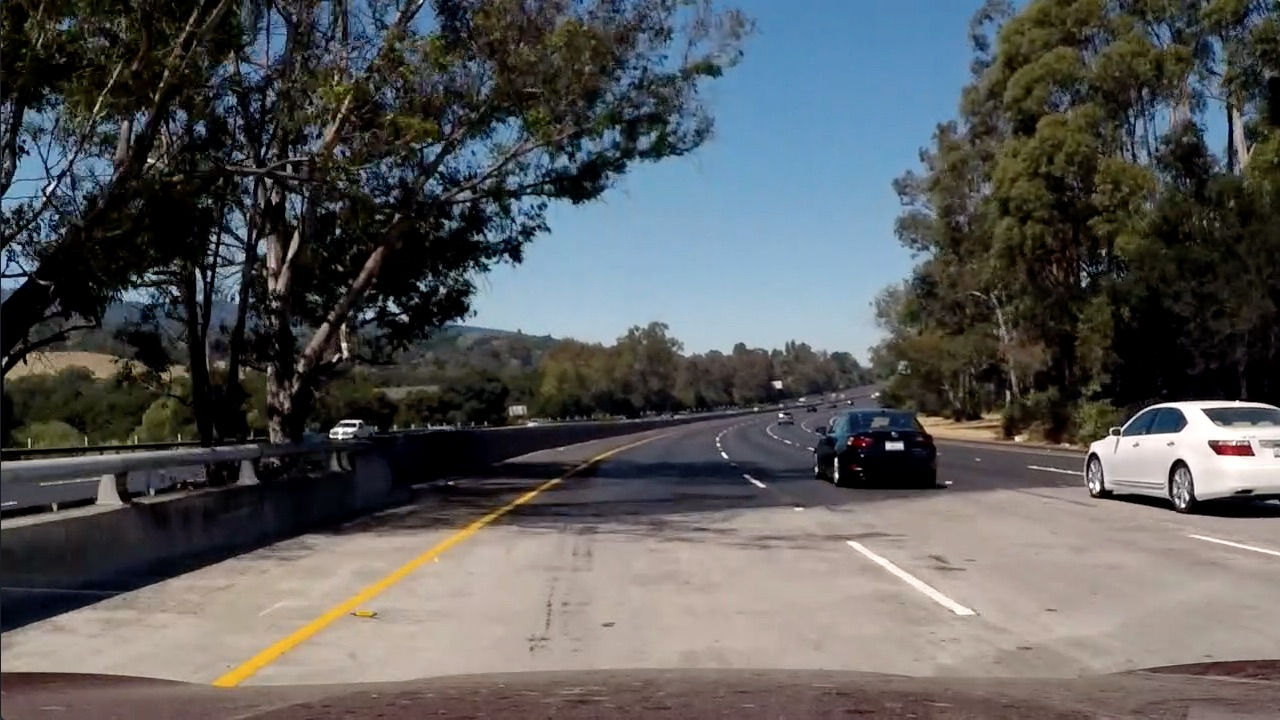
\includegraphics[width = 7cm]{images/test5}}
				{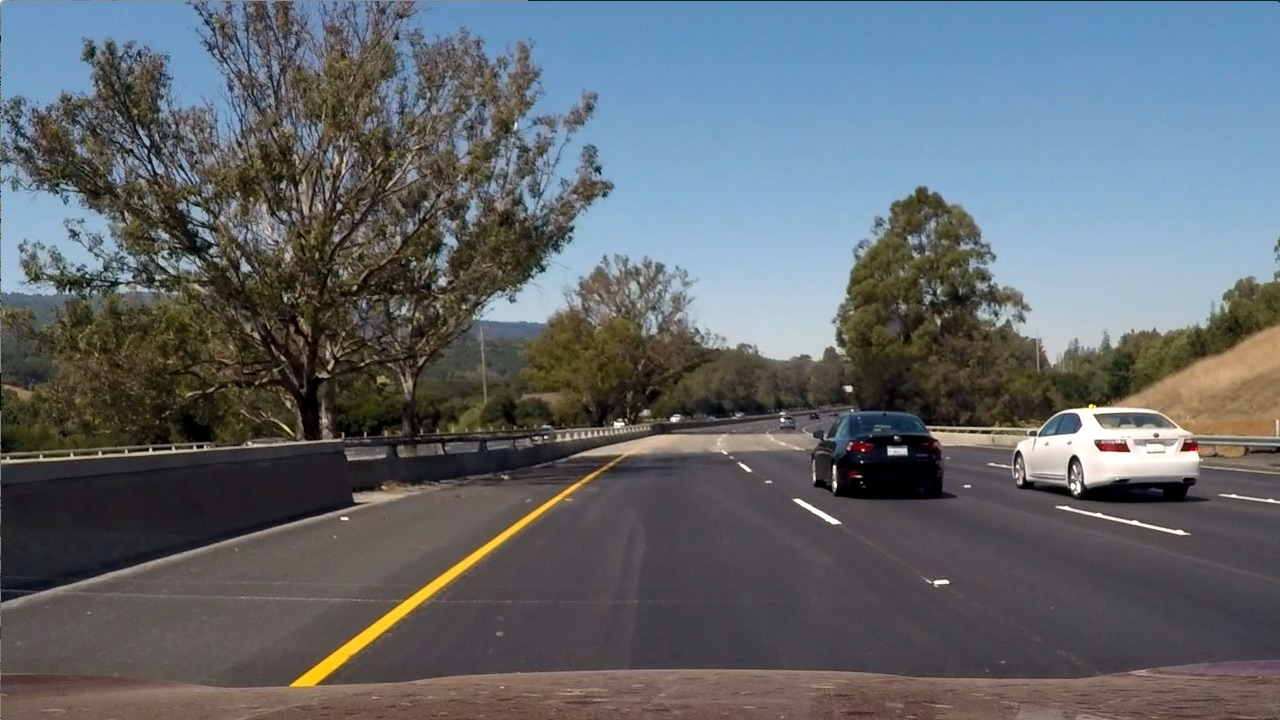
\includegraphics[width = 7cm]{images/test6}}\\
			\end{figure} \\
			\hline
		\end{tabular}
	\end{adjustbox}
	\captionof{figure}{Citra untuk deteksi kendaraan}
	\label{fig:ContohDataDeteksi}
\end{table}

\subsection{Implementasi Proses Latih}
Pelatihan yang dilakukan merupakan proses klasifikasi dimana membedakan objek mobil dan bukan mobil. Berikut ini adalah uraian dari proses pelatihan yang dilakukan dalam penelitian ini:
\begin{enumerate}
	\item \textit{Dataset} dimuat dan dikelompokkan mejadi mobil dan bukan mobil.
	\item Menentukan semua parameter yang dibutuhkan.
	\item Melakukan ekstraksi fitur kepada seluruh \textit{dataset}.
	\item Menyatukan dan melakukan normalisasi terhadap fitur.
	\item Fitur dari \textit{dataset} kemudian diacak dan dibagi menjadi 70\% untuk pelatihan, dan 30\% untuk pengujian.
	\item Melakukan pelatihan proses klasifikasi SVM menggunakan fitur dari data latih.
	\item Menyimpan hasil klasifikasi HOG dalam \textit{pickle file}.
	\\
\end{enumerate}

\subsection{Implementasi Proses Uji}
Pada bagian ini, akan dilakukan berbagai skenario pengujian dengan beragam parameter dari metode HOG. Tujuan dari penelitian ini adalah untuk menerapkan metode \textit{HOG} pada proses ekstraksi fitur, oleh karena itu perlu diketahui beberapa parameter masukkan yaitu ukuran sel, ukuran blok, dan jumlah \textit{bin} untuk menghasilkan fitur dan akurasi pengenalan karakter yang terbaik. Pengujian ini akan dilakukan dengan data latih sebanyak 6 buah citra yang diambil dari video. 6 buah citra ini didapat dari dataset dan sudah meliputi seluruh keadaan kondisi lokasi penelitian.\\

\subsection{Implementasi Aplikasi}
Bagian ini menjelaskan tampilan \textit{Graphical User Interface} (GUI) yang terdapat dalam aplikasi deteksi mobil dari citra kamera yang diambil dari \textit{dashboard} mobil. Tampulan GUI berguna untuk memudahkan user dalam melakukan proses uji. Tampilan dibuat berbasis \textit{desktop} menggunakan bahasa program python. Berikut adalah tampilan dari aplikasi deteksi mobil:
\\

\subsection{Skenario Pengujian}
Pada tahap ini, akan dijelaskan mengenai pengujian yang dilakukan dengan aplikasi yang telah dibuat. Hasil dari pengujian ini adalah untuk mendapatkan hasil klasifikasi untuk deteksi mobil menggunakan metode HOG.
\\

\subsubsection{Pengujian Kombinasi Parameter}
Bagian ini akan menjelaskan pengujian dengan beragam kombinasi parameter metode HOG dalam proses ekstraksi fitur. Fitur dari metode \textit{HOG} akan digunakan pada proses klasifikasi dan deteksi dengan nilai dari setiap parameter yang akan digunakan untuk kombinasi meliputi:
\begin{enumerate}
	\item Ukuran sel yang akan digunakan : 2, 4, 8, 16
	\item Ukuran blok yang akan digunakan : 4, 8, 16, 32
	\item Jumlah \textit{bin} yang akan digunakan : 4, 6, 9, 18
\end{enumerate}
Untuk nilai sigma pada metode \textit{SVM} yang digunakan dalam kombinasi adalah 0.01, 0.1, dan 1. Hasil kemudian akan diukur akurasinya menggunakan \textit{Confusion Matrix}.\\

\subsubsection{Pengujian dengan Ukuran Sel 2}
Bagian ini akan menjelaskan pengujian terhadap akurasi dengan menggunakan ukuran sel 2 $\times$ 2 piksel dan ukuran blok 2 $\times$ 2 sel (4 $\times$ 4 piksel). Dalam penelitian ini, jumlah bin yang akan digunakan adalah 4, 6, 9, dan 18 dan untuk nilai sigma pada metode \textit{SVM} yang akan digunakan adalah 0.01, 0.1, dan 1. Berikut adalah hasil pengujian untuk setiap kombinasi parameter tersebut:
\begin{longtable}[c]{|c|c|c|}
	\caption{Hasil Pengujian dengan ukuran sel 2 $\times$ 2 piksel}
	\label{tab:HasilPengujianSel2}\\
	\hline
	\begin{tabular}[c]{@{}c@{}}Parameter\\ (CellSize, NumBins, Sigma)\end{tabular} & CRR     & OVR     \\ \hline
	\endhead
	%
	(2, 4, 0.01)                                                                   & {\color[HTML]{FE0000} 58.52\%} & {\color[HTML]{FE0000} 10.34\%} \\ \hline
	(2, 4, 0.1)                                                                    & 26.13\% & 0\%     \\ \hline
	(2, 4, 1)                                                                      & 18.18\% & 0\%     \\ \hline
	(2, 6, 0.01)                                                                   & 50\%    & 6.89\%  \\ \hline
	(2, 6, 0.1)                                                                    & 25.56\% & 0\%     \\ \hline
	(2, 6, 1)                                                                      & 18.18\% & 0\%     \\ \hline
	(2, 9, 0.01)                                                                   & 48.29\% & 3.44\%  \\ \hline
	(2, 9, 0.1)                                                                    & 25\%    & 0\%     \\ \hline
	(2, 9, 1)                                                                      & 18.18\% & 0\%     \\ \hline
	(2, 18, 0.01)                                                                  & 44.88\% & 3.44\%  \\ \hline
	(2, 18, 0.1)                                                                   & 25\%    & 0\%     \\ \hline
	(2, 18, 1)                                                                     & 18.18\% & 0\%     \\ \hline
\end{longtable}
Berdasarkan tabel di atas, dapat disimpulkan bahwa akurasi pengenalan karakter maksimal yang didapatkan apabila menggunakan ukuran sel 2 $\times$ 2 piksel adalah 58.52\%. Kombinasi parameter yang digunakan untuk mencapai hasil tersebut adalah ukuran sel 2 $\times$ 2 piksel, jumlah \textit{bin} sebanyak 4 sehingga besar setiap \textit{bin} adalah 45 derajat, kemudian nilai \textit{sigma} yang digunakan untuk metode \textit{SVM} adalah 0.01. Dengan citra karakter inputan berukuran 32 $\times$ 32 piksel. Maka panjang vektor fitur dari \textit{HOG descriptor} yang dihasilkan adalah 3600 fitur.

Kolom di bagian kiri menunjukkan kombinasi parameter yang digunakan pada saat pengujian. Kolom CRR merupakan akronim dari \textit{Character Recognition Rate} yang memiliki rumus jumlah karakter yang dikenali dibagi dengan keseluruhan karakter yang terdeteksi. Dari 176 karakter yang terdeteksi, sebanyak 103 di antaranya dapat diklasifikasikan dengan baik. Kolom OVR pada bagian kanan menunjukkan performa keseluruhan yang memiliki rumus jumlah plat nomor yang terdeteksi dan dikenali dengan benar dibagi dengan keseluruhan jumlah plat nomor yang ada. Dari 29 plat nomor yang terdeteksi, hanya 3 plat nomor yang dapat dikenali dengan baik. Dapat disimpulkan bahwa penggunaan ukuran sel 2 $\times$ 2 piksel kurang tepat untuk kasus ini.\\

\subsubsection{Pengujian dengan Ukuran Sel 4}
Pada bagian ini, pengujian akan dilakukan dengan menggunakan ukuran sel berukuran 4 $\times$ 4 piksel dan ukuran blok 2 $\times$ 2 sel (8 $\times$ 8 piksel). Jumlah bin yang akan digunakan adalah 4, 6, 9, dan 18. Sedangkan untuk nilai sigma pada metode \textit{SVM} yang akan digunakan adalah 0.01, 0.1, dan 1. Berikut adalah hasil pengujian untuk setiap kombinasi parameter tersebut:
\begin{longtable}[c]{|c|c|c|}
	\caption{Hasil Pengujian dengan ukuran sel 4 $\times$ 4 piksel}
	\label{tab:HasilPengujianSel4}\\
	\hline
	\begin{tabular}[c]{@{}c@{}}Parameter\\ (CellSize, NumBins, Sigma)\end{tabular} & CRR     & OVR     \\ \hline
	\endhead
	%
	(4, 4, 0.01)                                                                   & 86.36\% & 27.58\% \\ \hline
	(4, 4, 0.1)                                                                    & 47.72\% & 0\%     \\ \hline
	(4, 4, 1)                                                                      & 26.13\% & 0\%     \\ \hline
	(4, 6, 0.01)                                                                   & 85.22\% & 31.03\%  \\ \hline
	(4, 6, 0.1)                                                                    & 40.90\% & 0\%     \\ \hline
	(4, 6, 1)                                                                      & 25\%    & 0\%     \\ \hline
	(4, 9, 0.01)                                                                   & {\color[HTML]{FE0000} 89.77\%} & {\color[HTML]{FE0000} 37.93\%}  \\ \hline
	(4, 9, 0.1)                                                                    & 40.90\% & 0\%     \\ \hline
	(4, 9, 1)                                                                      & 23.86\% & 0\%     \\ \hline
	(4, 18, 0.01)                                                                  & 84.09\% & 34.48\%  \\ \hline
	(4, 18, 0.1)                                                                   & 40.90\% & 0\%     \\ \hline
	(4, 18, 1)                                                                     & 24.43\% & 0\%     \\ \hline
\end{longtable}
Berdasarkan tabel di atas, dapat disimpulkan bahwa akurasi pengenalan karakter maksimal yang didapatkan apabila menggunakan ukuran sel 4 $\times$ 4 piksel adalah 89.77\%. Kombinasi parameter yang digunakan untuk mencapai hasil tersebut adalah ukuran sel 4 $\times$ 4 piksel, jumlah \textit{bin} sebanyak 9 sehingga besar setiap \textit{bin} adalah 20 derajat, kemudian nilai \textit{sigma} yang digunakan untuk metode \textit{SVM} adalah 0.01. Dengan citra karakter inputan berukuran 32 $\times$ 32 piksel. Maka panjang vektor fitur dari \textit{HOG descriptor} yang dihasilkan adalah 1764 fitur. Jika dibandingkan dengan pengujian sebelumnya, jumlah fitur yang lebih sedikit justru mampu mendapatkan akurasi pengenalan karakter yang lebih baik.

Sama seperti bagian sebelumnya, kolom di bagian kiri menunjukkan kombinasi parameter yang digunakan pada saat pengujian. Dari hasil pada kolom CRR, dari 176 karakter yang terdeteksi, sebanyak 158 di antaranya dapat diklasifikasikan dengan baik. Dari hasil pada kolom OVR menunjukkan, dari 29 plat nomor yang terdeteksi, 11 plat nomor dapat dikenali dengan baik, hal ini merupakan peningkatan apabila dibandingkan dengan hasil pengujian sebelumnya, namun masih cukup banyak plat yang tidak dapat dikenali dengan baik. Dari pengujian ini dapat  disimpulkan bahwa penggunaan ukuran sel 4 $\times$ 4 piksel sudah dapat meningkatkan akurasi pengenalan karakter namun masih belum optimal.\\

\subsubsection{Pengujian dengan Ukuran Sel 8}
Pada bagian ini, pengujian akan dilakukan dengan menggunakan ukuran sel berukuran 8 $\times$ 8 piksel dan ukuran blok 2 $\times$ 2 sel (16 $\times$ 16 piksel). Jumlah bin yang akan digunakan adalah 4, 6, 9, dan 18. Sedangkan untuk nilai sigma pada metode \textit{SVM} yang akan digunakan adalah 0.01, 0.1, dan 1. Berikut adalah hasil pengujian untuk setiap kombinasi parameter tersebut:
\begin{longtable}[c]{|c|c|c|}
	\caption{Hasil Pengujian dengan ukuran sel 8 $\times$ 8 piksel}
	\label{tab:HasilPengujianSel8}\\
	\hline
	\begin{tabular}[c]{@{}c@{}}Parameter\\ (CellSize, NumBins, Sigma)\end{tabular} & CRR     & OVR     \\ \hline
	\endhead
	%
	(8, 4, 0.01)                                                                   & 15.90\% & 0\% \\ \hline
	(8, 4, 0.1)                                                                    & 93.18\% & 51.72\%     \\ \hline
	(8, 4, 1)                                                                      & 46.02\% & 0\%     \\ \hline
	(8, 6, 0.01)                                                                   & 21.02\% & 0\%  \\ \hline
	(8, 6, 0.1)                                                                    & 93.18\% & 51.72\%     \\ \hline
	(8, 6, 1)                                                                      & 42.61\% & 0\%     \\ \hline
	(8, 9, 0.01)                                                                   & 28.40\% & 0\%  \\ \hline
	(8, 9, 0.1)                                                                    & 93.75\% & 51.72\%     \\ \hline
	(8, 9, 1)                                                                      & 39.20\% & 0\%     \\ \hline
	(8, 18, 0.01)                                                                  & 21.59\% & 0\%  \\ \hline
	(8, 18, 0.1)                                                                   & {\color[HTML]{FE0000} 94.88\%} & {\color[HTML]{FE0000} 58.62\%}     \\ \hline
	(8, 18, 1)                                                                     & 40.34\% & 0\%     \\ \hline
\end{longtable}
Berdasarkan tabel di atas, dapat disimpulkan bahwa akurasi pengenalan karakter maksimal yang didapatkan apabila menggunakan ukuran sel 8 $\times$ 8 piksel adalah 94.88\%. Kombinasi parameter yang digunakan untuk mencapai hasil tersebut adalah ukuran sel 8 $\times$ 8 piksel, jumlah \textit{bin} sebanyak 18 sehingga besar setiap \textit{bin} adalah 10 derajat, kemudian nilai \textit{sigma} yang digunakan untuk metode \textit{SVM} adalah 0.1. Dengan citra karakter inputan berukuran 32 $\times$ 32 piksel. Maka panjang vektor fitur dari \textit{HOG descriptor} yang dihasilkan adalah 648 fitur. Sama seperti pengujian sebelumnya, jika dibandingkan dengan pengujian sebelumnya, jumlah fitur yang lebih sedikit justru mampu mendapatkan akurasi pengenalan karakter yang lebih baik.

Sama seperti bagian sebelumnya, kolom di bagian kiri menunjukkan kombinasi parameter yang digunakan pada saat pengujian. Dari hasil pada kolom CRR, dari 176 karakter yang terdeteksi, sebanyak 167 di antaranya dapat diklasifikasikan dengan baik. Dari hasil pada kolom OVR menunjukkan, dari 29 plat nomor yang terdeteksi, 17 plat nomor dapat dikenali dengan baik, hal ini merupakan peningkatan apabila dibandingkan dengan hasil pengujian sebelumnya, dengan memperhatikan akurasi pengenalan karakter yang tinggi namun hasil performa keseluruhan yang masih di bawah 70\% maka dapat disimpulkan bahwa kemungkinan ada faktor lain yang cukup menghambat dalam proses pengenalan karakter pada keseluruhan plat nomor. Dari pengujian ini dapat  disimpulkan bahwa penggunaan ukuran sel 8 $\times$ 8 piksel sudah dapat menghasilkan akurasi pengenalan karakter yang baik.\\

\subsubsection{Pengujian dengan Ukuran Sel 16}
Pada bagian ini, pengujian akan dilakukan dengan menggunakan ukuran sel berukuran 16 $\times$ 16 piksel dan ukuran blok 2 $\times$ 2 sel (32 $\times$ 32 piksel). Jumlah bin yang akan digunakan adalah 4, 6, 9, dan 18. Sedangkan untuk nilai sigma pada metode \textit{SVM} yang akan digunakan adalah 0.01, 0.1, dan 1. Berikut adalah hasil pengujian untuk setiap kombinasi parameter tersebut:
\begin{longtable}[c]{|c|c|c|}
	\caption{Hasil Pengujian dengan ukuran sel 16 $\times$ 16 piksel}
	\label{tab:HasilPengujianSel16}\\
	\hline
	\begin{tabular}[c]{@{}c@{}}Parameter\\ (CellSize, NumBins, Sigma)\end{tabular} & CRR     & OVR     \\ \hline
	\endhead
	%
	(16, 4, 0.01)                                                                   & 13.06\% & 0\% \\ \hline
	(16, 4, 0.1)                                                                    & 18.75\% & 0\%     \\ \hline
	(16, 4, 1)                                                                      & 84.09\% & 17.24\%     \\ \hline
	(16, 6, 0.01)                                                                   & 13.06\% & 0\%  \\ \hline
	(16, 6, 0.1)                                                                    & 22.72\% & 0\%     \\ \hline
	(16, 6, 1)                                                                      & 84.09\% & 13.79\%     \\ \hline
	(16, 9, 0.01)                                                                   & 13.06\% & 0\%  \\ \hline
	(16, 9, 0.1)                                                                    & 28.97\% & 0\%     \\ \hline
	(16, 9, 1)                                                                      & {\color[HTML]{FE0000} 86.36\%} & {\color[HTML]{FE0000} 27.58\%}     \\ \hline
	(16, 18, 0.01)                                                                  & 13.06\% & 0\%  \\ \hline
	(16, 18, 0.1)                                                                   & 23.29\% & 0\%     \\ \hline
	(16, 18, 1)                                                                     & 85.79\% & 24.13\%     \\ \hline
\end{longtable}
Berdasarkan tabel di atas, dapat disimpulkan bahwa akurasi pengenalan karakter maksimal yang didapatkan apabila menggunakan ukuran sel 16 $\times$ 16 piksel adalah 86.36\%. Kombinasi parameter yang digunakan untuk mencapai hasil tersebut adalah ukuran sel 16 $\times$ 16 piksel, jumlah \textit{bin} sebanyak 9 sehingga besar setiap \textit{bin} adalah 20 derajat, kemudian nilai \textit{sigma} yang digunakan untuk metode \textit{SVM} adalah 1. Dengan citra karakter inputan berukuran 32 $\times$ 32 piksel. Maka panjang vektor fitur dari \textit{HOG descriptor} yang dihasilkan adalah 9 fitur. Berbeda dengan pengujian sebelumnya, kali ini jumlah fitur yang terlalu sedikit justru akan mengurangi akurasi dari proses pengenalan karakter yang sebelumnya sudah mencapai 94.88\%, dari keseluruhan pengujian yang sudah dilakukan terhadap jumlah sel, dapat disimpulkan bahwa ukuran sel yang terlampau besar ataupun terlampau kecil pada penggunaan metode \textit{HOG} dapat mengurangi kualitas fitur yang dihasilkan sehingga akan berefek terhadap hasil klasifikasi.

Sama seperti bagian sebelumnya, kolom di bagian kiri menunjukkan kombinasi parameter yang digunakan pada saat pengujian. Dari hasil pada kolom CRR, dari 176 karakter yang terdeteksi, sebanyak 152 di antaranya dapat diklasifikasikan dengan baik. Dari hasil pada kolom OVR menunjukkan, dari 29 plat nomor yang terdeteksi, 8 plat nomor dapat dikenali dengan baik, hal ini merupakan dampak dari penurunan akurasi pengenalan karakter. Dari pengujian ini dapat  disimpulkan bahwa penggunaan ukuran sel 16 $\times$ 16 piksel dapat menghasilkan akurasi pengenalan karakter yang baik namun belum optimal.\\

\newpage
%%-----------------------------------------------------------------------------%
\chapter{PENUTUP}
%-----------------------------------------------------------------------------%

%
\vspace{4.5pt}

\section{Kesimpulan}

\section{Saran}

\newpage

\lhead{\leftmark}
\renewcommand{\headrulewidth}{1pt}

\fancypagestyle{plain}{%
	\renewcommand{\headrulewidth}{0pt}%
	\fancyhf{}%
	\fancyfoot[R]{\arabic{chapter}-1}%
}

\onehalfspacing
\setcounter{page}{1}
\rfoot{\arabic{chapter}-\arabic{page}}
%-----------------------------------------------------------------------------%
\chapter{PENDAHULUAN}
%-----------------------------------------------------------------------------%

\vspace{4.5pt}

\section{Latar Belakang} \label{sec:latar_belakang}

Kemajuan teknologi di bidang transportasi membantu manusia dalam berpindah tempat antar lokasi dalam waktu singkat. Kemajuan teknologi ini dapat dilihat pada teknologi yang digunakan pada kendaraan bermotor seperti penggunaan sistem kemudi otomatis atau \textit{self driving}. Pentingnya sistem kemudi otomatis adalah untuk membantu manusia meringkankan pekerjaan dalam mengemudi dan menurunkan potensi kecelakaan akibat kelelahan dalam menyetir \cite{bougharriou}. Sistem kemudi otomatis membutuhkan deteksi objek. Salah satu objek yang perlu di deteksi adalah mobil. Proses deteksi mobil diawali dengan pengambilan citra dari \textit{dashboard} mobil, kemudian citra diproses untuk setiap \textit{frame}. Dari setiap frame yang diperoleh kemudian diolah untuk mendeteksi posisi mobil, sehingga kecelakaan dapat dihindari.
 
Proses deteksi mobil meliputi tahap \textit{preprocessing}, ekstraksi fitur, tahap klasifikasi. Tahap \textit{preprocessing} berfungsi untuk mendeteksi \textit{Region of Interest} (ROI), yaitu daerah dimana proses deteksi dilakukan dan juga untuk menentukan arah darimana citra diambil. Tahap ekstraksi fitur berfungsi untuk mengambil ciri dari citra untuk digunakan dalam membedakan objek. Tahap morfologi berfungsi untuk mengurangi jumlah objek dengan menghilangkan objek yang tidak sesuai kategori. Sedangkan tahap klasifikasi menentukan dan mengelompokkan objek yang serupa. Mobil yang telah dideteksi dihitung dan ditandai.

\textit{Preprocessing} yang dilakukan yaitu \textit{grayscalling} dan menentukan ROI untuk memperkecil penggunaan memori \cite{prahara}. ROI yang dimaksud berupa jalan dimana mobil akan melaju. ROI yang digunakan, dibuat secara manual berupa citra biner berdasarkan data latih yang digunakan.

Banyak penelitian telah meneliti metode yang akan digunakan untuk deteksi mobil, diantaranya adalah Haar-like, LBP, dan HOG. Metode ini merupakan \textit{Feature Based Methods} yang direpresentasikan dengan baik untuk ekstraksi fitur. Berdasarkan penelitian yang dilakukan oleh \cite{neumann}, pendekatan berbasis fitur HOG mencapai hasil terbaik sehingga akan digunakan pada penelitian ini. Dengan fitur LBP, ditemukan banyak \textit{false positives} yang terdeteksi. Fitur seperti Haar berkinerja terburuk, yang mungkin disebabkan oleh keragaman model sehingga mencegah kecocokan yang baik untuk area pola yang jernih dan berbayang \cite{neumann}.

SVM (\textit{Support Vector Machine}), kNN (\textit{k nearest neighborhood}), dan RF (\textit{Random Forest}) merupakan metode klasifikasi yang populer. Ketiga metode ini menghasilkan hasil yang baik, tetapi performa kNN menurun ketika ruang fitur tidak stabil dan RF tidak bekerja baik pada ruang vektor yang rumit. SVM terbukti dapat menangani masalah klasifikasi dengan efisien \cite{sajib}. Dikarenakan metode SVM memiliki efisiensi yang cukup baik dan cocok dengan metode HOG dengan akurasi sebesar 83\% \cite{shakin}, maka ditentukan \textit{classifier} untuk penelitian ini menggunakan metode SVM.

Pada penelitian ini, \textit{dataset} yang digunakan adalah citra mobil. Dataset yang digunakan terdiri dari 3 jenis data latih yang diambil dari sumber yang berbeda. Penelitian ini menggunakan \textit{dataset UIUC Car Image Database}, \textit{GTI Database}, dan \textit{KITTI Database}. Arah pengambilan kamera untuk \textit{dataset} dilakukan dari posisi \textit{horizontal}. Untuk data latih dibagi menjadi 2 jenis yaitu mobil (kondisi utuh, tidak ada bagian mobil yang terpotong) dan bukan mobil (jalanan, motor, rumah, pejalan kaki, dan sebagainya). Kemudian untuk proses pengujian akan dilakukan analisis untuk kasus kondisi mobil dimana fitur yang terdapat pada citra uji tidak utuh. Pada dataset juga terdapat \textit{template} untuk \textit{Region of Interest} dimana berupa citra biner yang berfungsi untuk menandai lokasi dimana mobil akan melaju yang kemudian dimanfaatkan untuk daerah deteksi mobil.
\\

\section{Rumusan Masalah}
Berdasarkan latar belakang yang telah diuraikan di atas, terdapat beberapa permasalah yang dapat dirumuskan sebagai berikut:
\begin{enumerate}[nolistsep,leftmargin=0.5cm]
	\item 
	Bagaimana menentukan \textit{Region of Interest} yang tepat berdasarkan posisi kamera CCTV?
	\item 
	Berapa nilai akurasi pada hasil ekstraksi fitur dengan menggunakan metode \textit{Histogram of Oriented Gradients} dan klasifikasi menggunakan metode \textit{Support Vector Machine} untuk deteksi mobil?
	\\
\end{enumerate}

\section{Tujuan Penelitian}

Berdasarkan rumusan masalah di atas, maka dapat dideskripsikan tujuan dari penelitian ini, yaitu:
\begin{enumerate}[nolistsep,leftmargin=0.5cm]
	\item 
	Menentukan \textit{Region of Interest} yang sesuai terhadap posisi kamera CCTV.
	\item 
	Melakukan penerapan metode \textit{Histogram of Oriented Gradients} dan \textit{Support Vector Machine} pada sistem deteksi mobil.
	\item
	Menghitung nilai akurasi deteksi mobil dengan menggunakan metode \textit{Confusion Matrix}.
	\\
\end{enumerate}

\section{Batasan Masalah}

Agar penelitian ini lebih fokus dan terarah, maka penulis akan memberikan beberapa batasan masalah sebagai berikut:
\begin{enumerate}[nolistsep,leftmargin=0.5cm]
	\item 
	\textit{Region of Interest} (ROI) yang digunakan adalah jalan raya dimana mobil melaju berdasarkan posisi kamera CCTV di \textit{dashboard} mobil.
	\item
	Dataset yang digunakan adalah citra mobil, merupakan citra \textit{grayscale} dengan ekstensi PGM berukuran 64 x 64 piksel dengan \textit{depth bit} 8. 
	\item
	Posisi pengambilan citra hanya dilakukan dari belakang mobil saja, yang terdiri dari 4 bagian yaitu jauh, dekat, kiri, dan kanan.
	\\
\end{enumerate}

\section{Kontribusi Penelitian}
Menerapkan metode \textit{Histogram of Oriented Gradients} untuk melakukan ekstraksi fitur pada citra dan \textit{Support Vector Machine} untuk melakukan klasifikasi objek.\\

\section{Metodologi Penelitian}

Berikut ini merupakan metodologi penelitian yang dilakukan dalam penelitian ini: 
\begin{enumerate}[nolistsep,leftmargin=0.5cm]
%	\item 
%	Tinjauan Pustaka \\
%	Mengumpulkan data dan informasi dengan menggunakan referensi pustaka yang berasal dari berbagai media dan sumber (artikel, buku, literatur, jurnal, tugas akhir, dan \textit{thesis}) yang berhubungan dengan penelitian yang dilakukan dan metode yang digunakan.
	
	\item
	Pengumpulan Data \\
	Data latih yang digunakan berupa citra digital yang diambil dari \textit{http://cogcomp.org/Data/Car/, http://www.gti.ssr.upm.es/data/Vehicle\_database.html, dan http://www.cvlibs.net/datasets/kitti/} dan data uji berupa citra video dari \textit{http://www.youtube.com.}
	
	\item
	Analisis dan Perancangan \\
	Menganalisis dan merancang sistem yang akan dibuat berdasarkan \textit{dataset} yang sudah diperoleh sebelumnya.
	
	\item
	Implementasi \\
	Mengimplementasikan hasil perancangan yang telah dibuat sebelumnya dalam bentuk aplikasi untuk melakukan ekstraksi fitur.
	
	\item
	Pengujian \\
	Melakukan pengujian terhadap aplikasi yang telah dibuat dan menghitung nilai akurasi dari hasil deteksi mobil. Selain itu akan dilakukan pengujian untuk kasis fitur tidak utuh dan analisis setiap \textit{parameter} masukan pada setiap metode untuk mendapatkan nilai dari \textit{parameter} yang sesuai untuk kasus \textit{dataset} mobil.
	\\
\end{enumerate}

\section{Sistematika Penulisan}

Laporan penelitian ini disusun berdasarkan sistematika penulisan berikut ini: \\[0.5cm]
\noindent 
\textbf{BAB I \hspace{1cm} Pendahuluan}
\begin{addmargin}[2.35cm]{0em}
Bab ini menjelaskan tentang latar belakang, rumusan masalah, tujuan penelitian, batasan masalah, metodologi penelitian, dan sistematika penulisan.
\end{addmargin}
\noindent 
\textbf{BAB II \hspace{0.8cm} Landasan Teori}
\begin{addmargin}[2.35cm]{0em}
Bab ini menjelaskan teori mengenai tinjauan pustaka, tinjauan studi, dan tinjauan objek.
\end{addmargin}
\noindent 
\textbf{BAB III \hspace{0.7cm} Analisis dan Perancangan}
\begin{addmargin}[2.35cm]{0em}
Bab ini menjelaskan analisa terhadap masalah, solusi, dan perancangan sistem.
\end{addmargin}
\noindent 
\textbf{BAB IV \hspace{0.7cm} Implementasi dan Pengujian}
\begin{addmargin}[2.35cm]{0em}
Bab ini menjelaskan proses implementasi dan pengujian terhadap aplikasi yang dibuat.
\end{addmargin}
\noindent \textbf{BAB V \hspace{0.8cm} Kesimpulan dan Saran}
\begin{addmargin}[2.35cm]{0em}
Bab ini menjelaskan kesimpulan dari aplikasi yang telah dibuat dan saran untuk pengembangan aplikasi lain.
\end{addmargin}

\newpage
\setcounter{page}{1}
%-----------------------------------------------------------------------------%
\chapter{LANDASAN TEORI}
%-----------------------------------------------------------------------------%

%
\vspace{4.5pt}

\section{Tinjauan Pustaka}
Pada bagian ini akan membahas teori-teori terkait yang digunakan pada penelitian ini.
\\

\subsection{Citra Digital}
Citra digital merupakan representasi dari fungsi intensitas cahaya dalam bentuk diskrit pada bidang dua dimensi. Citra tersusun oleh sekumpulan piksel (\textit{picture element}) yang memiliki koordinat (x,y) dan intensitas f(x,y). Koordinat (x,y) menunjukkan letak/posisi piksel dalam suatu citra, sedangkan intensitas f(x,y) menunjukkan nilai intensitas warna citra \cite{gonzalez}. Untuk membuat citra digital, diperlukan pengubahan data pengindraan kontinu menjadi bentuk digital. Tahap ini melibatkan dua proses, yaitu pengambilan sampel dan kuantisasi. Gambar \ref{img:CitraDigital} merupakan contoh dari citra digital.

\begin{table}[H]
	\small
	\begin{adjustbox}{width=1\textwidth}
		\begin{tabular}{| p {14cm} |}
			\hline
			\begin{figure}[H]
				\centering
				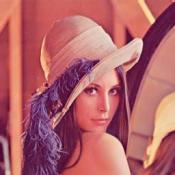
\includegraphics[width=7cm]{images/rgb.jpg}
			\end{figure} \\
			\hline
		\end{tabular}
	\end{adjustbox}
	\captionof{figure}{Contoh Citra Digital \cite{gonzalez}}
	\label{img:CitraDigital}
\end{table}

Suatu citra dapat bersifat kontinu sehubungan dengan koordinat x dan y, dan juga dalam intensitas. Untuk mengubahnya menjadi bentuk digital, harus dicoba fungsi dalam koordinat dan intensitas. \textit{Sampling} adalah proses untuk menentukan warna pada piksel tertentu pada citra dari sebuah gambar yang kontinu. Pada proses \textit{sampling} biasanya dicari warna rata-rata dari gambar analog yang kemudian dibulatkan. Proses \textit{sampling} sering juga disebut proses digitalisasi. \textit{Sampling} merupakan bagian dari metodologi statistika. Adakalanya, dalam proses \textit{sampling}, warna rata-rata yang didapat di relasikan ke level warna tertentu. Contohnya apabila dalam citra hanya terdapat 16 tingkatan warna abu-abu, maka nilai rata-rata yang didapat dari proses sampling harus diasosiasikan ke 16 tingkatan tersebut. Proses mengasosiasikan warna rata-rata dengan tingkatan warna tertentu disebut dengan kuantisasi.
\\ 

\subsection{Pengolahan Citra}
Pengolahan citra adalah salah satu cabang dari ilmu informatika (Komputer). Pengolahan citra berfokus pada usaha untuk melakukan transformasi suatu citra/gambar menjadi citra lain dengan menggunakan teknik tertentu. Berikut ini merupakan langkah-langkah yang umumnya dilakukan dalam merancang sebuah sistem pengolahan citra dan pengenalan pola:

\begin{table}[H]
	\small
	\begin{adjustbox}{width=1\textwidth}
		\begin{tabular}{| p {14cm} |}
			\hline
			\begin{figure}[H]
				\centering
				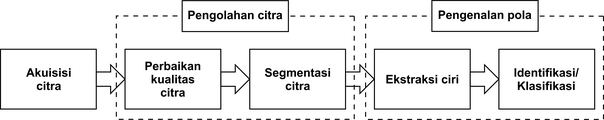
\includegraphics[width=14cm]{images/pencit}
			\end{figure} \\
			\hline
		\end{tabular}
	\end{adjustbox}
	\captionof{figure}{Proses Pengolahan Citra dan Pengenalan Pola}
	\label{img:pencit}
\end{table}

Operasi yang dilakukan untuk mengubah suatu citra menjadi citra lain dapat dikategorikan berdasarkan tujuan transformasi maupun cakupan operasi yang dilakukan terhadap citra. Berdasarkan tujuan transformasi operasi pengolahan citra dikategorikan menjadi peningkatan kualitas citra (\textit{Image Enhancement}) dan pemulihan citra (image restoration). Operasi peningkatan kualitas citra bertujuan untuk meningkatkan fitur tertentu pada citra. Sedangkan operasi pemulihan citra bertujuan untuk mengembalikan kondisi citra pada kondisi yang diketahui sebelumnya akibat adanya \textit{noise} yang menyebabkan penurunan kualitas citra. Berdasarkan cakupan operasi yang dilakukan terhadap citra, operasi pengolahan citra dikategorikan menjadi operasi titik, lokal, dan global. 

Operasi titik merupakan operasi yang dilakukan terhadap setiap piksel pada citra yang keluarannya hanya ditentukan oleh nilai piksel itu sendiri. Operasi titik dapat dibagi menjadi tiga macam, yaitu berdasarkan intensitas, geometri, dan gabungan keduanya. Contoh operasi titik berdasar intensitas adalah operasi pengambangan (\textit{thresholding}) yaitu membuat citra biner, operasi negatif (\textit{negative image}) yaitu membuat citra negatif, pemotongan citra (\textit{clipping}), dan pencerahan citra (\textit{image brightening}) yaitu menambahkan atau mengurangi konstanta untuk memperbaiki kecerahan pada citra. Operasi lokal merupakan operasi yang dilakukan terhadap setiap piksel pada citra yang keluarannya dipengaruhi oleh piksel tersebut dan piksel lainnya dalam suatu daerah tertentu. Salah satu contoh dari operasi berbasis lokal adalah operasi konvolusi untuk mendeteksi tepi (\textit{edge detection}) an pelembutan citra (\textit{image smoothing}). Operasi global merupakan operasi yang dilakukan tehadap setiap piksel pada citra yang keluarannya ditentukan oleh keseluruhan piksel yang membentuk citra. Contoh operasi global adalah operasi penyetaraan histogram untuk meningkatkan kualitas citra.\\

\subsection{\textit{Preprocessing}}
\textit{Preprocessing} merupakan proses pengolahan data asli sebelum tahapan pengolahan data. Proses ini bertujuan agar data siap untuk diproses ke tahap ektraksi fitur. Preprocessing memiliki tujuan untuk menghilangkan derau, memperjelas fitur, mengubah ukuran citra, dan konversi data. Contoh dari \textit{preprocessing} yaitu pengabuan citra (\textit{grayscaling}), binerisasi citra, \textit{croping} citra, dan \textit{resize} citra \cite{gonzalez}.\\ 

\subsubsection{Pengabuan Citra}
Citra \textit{grayscale} adalah suatu citra yang hanya memiliki warna berupa tingkat keabuan. Citra \textit{grayscale} digunakan karena membutuhkan sedikit informasi yang diberikan pada tiap piksel dibandingkan dengan citra berwarna sehingga dalam \textit{grayscale} image hanya membutuhkan nilai intensitas tunggal dibandingkan dengan citra berwarna membutuhkan tiga intensitas untuk tiap pikselnya. Intensitas dari citra \textit{grayscale} disimpan dalam 8 bit integer yang memberikan 256 kemungkinan yang mana dimulai dari level 0 sampai dengan 255 (0 untuk hitam dan 255 untuk putih) \cite{gonzalez}. Gambar \ref{img:grayscale} merupakan contoh dari citra \textit{grayscale}.

\begin{table}[H]
	\small
	\begin{adjustbox}{width=1\textwidth}
		\begin{tabular}{| p {14cm} |}
			\hline
			\begin{figure}[H]
				\centering
				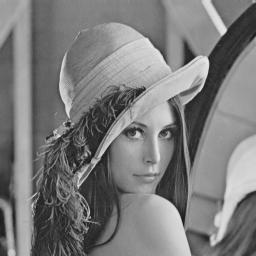
\includegraphics[width=7cm]{images/grayscale.jpg}
			\end{figure} \\
			\hline
		\end{tabular}
	\end{adjustbox}
	\captionof{figure}{Contoh Citra \textit{Grayscale} \cite{gonzalez}}
	\label{img:grayscale}
\end{table}

Persamaan pengabuan citra dapat dilihat pada persamaan \ref{eq:grayscale} dengan \textit{R} melambangkan intensitas warna merah, \textit{G} untuk intensitas warna hijau, dan \textit{B} untuk intensitas warna biru. 

\begin{table}[H]
	\begin{adjustbox}{width=1\textwidth}
		\begin{tabular}{|p{13.55cm}|}
			\hline
			\begin{equation}
			Gray value = 0.299 R + 0.587 G + 0.114 B
			\label{eq:grayscale}
			\end{equation}\\
			\hline
		\end{tabular}
	\end{adjustbox}
\end{table}

Persamaan \ref{eq:grayscale} menyimpulkan bahwa persentase warna hijau yang paling besar karena manusia cenderung lebih sensitif terhadap perubahan warna hijau yang memiliki panjang gelombang sekitar 500-570 nm, merah, lalu biru, dan merupakan rekomendasi dari \textit{International Telecommunication Union Radiocommunication Sector}.\\

\subsubsection{Citra Biner}
Citra biner (\textit{binary image}) adalah citra yang hanya mempunyai dua nilai derajat keabuan yaitu hitam dan putih. Citra biner bernilai 1 untuk objek dan 0 untuk latar belakang. Citra biner sering kali digunakan karena mempercepat waktu proses dan memperkecil penggunaan memori\cite{munir}. Meskipun komputer saat ini dapat memproses citra hitam-putih (\textit{grayscale}) maupun citra berwarna, namun citra biner masih tetap dipertahankan keberadaannya. 

\begin{table}[H]
	\small
	\begin{adjustbox}{width=1\textwidth}
		\begin{tabular}{| p {14cm} |}
			\hline
			\begin{figure}[H]
				\centering
				\includegraphics[width=7cm]{images/biner.jpg}
			\end{figure} \\
			\hline
		\end{tabular}
	\end{adjustbox}
	\captionof{figure}{Contoh Citra Biner \cite{gonzalez}.}
	\label{img:binary}
\end{table}

Sama seperti citra \textit{grayscale}, citra biner juga merupakan citra yang hanya memiliki satu kanal warna. Citra biner memiliki kedalaman bit sebesar 1-bit. \textit{Thresholding} adalah metode untuk mengubah citra \textit{grayscale} menjadi citra biner sehingga objek dapat dipisahkan dari \textit{background}. Untuk mendapat nilai \textit{threshold} yang adaptif menggunakan metode Otsu. Nilai intensitas warna pada setiap piksel citra biner dibagi menjadi 2$\land$1 = 2 warna yaitu warna hitam yang dinyatakan oleh nilai 0 dan warna putih yang dinyatakan oleh nilai 1. Persamaan yang digunakan untuk mengkonversi nilai piksel citra \textit{grayscale} menjadi biner pada metode \textit{thresholding} adalah:

\begin{table}[H]
	\small
	\begin{adjustbox}{width=1\textwidth}
		\begin{tabular}{|p{13.55cm}|}
			\hline
			\begin{equation} \label{eqn:biner}
			\displaystyle
			g(x,y) = \left\{\begin{array}{l}1, jika f(x,y) \ge T \\0, jika f(x,y) < T\end{array}\right.
			\end{equation} \\
			\hline
		\end{tabular}
	\end{adjustbox}
\end{table}

\noindent
\renewcommand{\arraystretch}{1}
\begin{tabularx}{\textwidth}{lll}
	\hline
	Keterangan: \\
	$g(x,y)$ & : & citra biner\\
	$f(x,y)$ & : & citra \textit{grayscale}\\
	$T$ & : & \textit{treshold}\\
	\hline
\end{tabularx}
\vspace{4.5pt} 

Citra biner digunakan saat proses penentuan ROI. ROI yang berupa citra biner digunakan untuk menandai lokasi dimana mobil akan melaju. ROI yang digunakan berupa template dari dataset yang diperoleh.\\

\subsubsection{\textit{Otsu Tresholding}}
Tujuan dari metode Otsu adalah membagi histogram citra gray level kedalam dua daerah yang berbeda secara otomatis tanpa membutuhkan bantuan pengguna untuk memasukkan nilai ambang. Pendekatan yang dilakukan oleh metode otsu adalah dengan melakukan analisis diskriminan yaitu menentukan suatu variabel (nilai ambang atau \textit{threshold}) yang dapat membedakan antara dua atau lebih kelompok yang muncul secara alami. Analisis Diskriminan akan memaksimumkan nilai ambang agar dapat membagi objek latar depan (\textit{foreground}) dan latar belakang (\textit{background}).

Langkah  awal  yang harus  dilakukan  adalah  membuat  histogram.  Dari histogram dapat diketahui jumlah piksel untuk setiap tingkat  keabuan.  Tingkat  keabuan  citra  dinyatakan dengan i sampai dengan L. Level ke i dimulai dari 1, yaitu  piksel  0.  Untuk L,  maksimal  level  adalah  256 dengan piksel bernilai 255. Nilai  ambang  yang  akan  dicari  dari  suatu  citra \textit{grayscale} dinyatakan dengan k. Nilai kberkisar antara 0  sampai  dengan L - 1,  dengan  nilai L = 256  (simbol histogram adalah Pi) \cite{otsu}. Jadi probabilitas setip piksel pada level ke i dinyatakan dengan persamaan berikut. 

\begin{table}[H]
	\small
	\begin{adjustbox}{width=1\textwidth}
		\begin{tabular}{|p{13.55cm}|}
			\hline
			\begin{equation} \label{eqn:otsu1}
			\displaystyle
			P_{i} = \frac{n_{i}}{N}
			\end{equation} \\
			\hline
		\end{tabular}
	\end{adjustbox}
\end{table}

\noindent
\renewcommand{\arraystretch}{1}
\begin{tabularx}{\textwidth}{lll}
	\hline
	Keterangan: \\
	$P_{i}$ & : & probabilitas piksel ke-i\\
	$n_{i}$ & : & jumlah piksel dengan tingkat keabuan i\\
	$N$ & : & total jumlah piksel pada citra\\
	\hline
\end{tabularx}
\vspace{4.5pt}

Langkah   selanjutnya   mencari   nilai   jumlah kumulatif, rerata  kumulatif  dan  intensitas  global. mencari  nilai  tersebut  dapat  melihat  persamaan  \eqref{eqn:otsu2}, persamaan \eqref{eqn:otsu3}, dan persamaan \eqref{eqn:otsu4}.

\begin{table}[H]
	\small
	\begin{adjustbox}{width=1\textwidth}
		\begin{tabular}{|p{13.55cm}|}
			\hline
			\begin{equation} \label{eqn:otsu2}
			\displaystyle
			\omega (k) = \sum\limits_{i=0}^{k} p_{i}
			\end{equation} 
			
			\begin{equation} \label{eqn:otsu3}
			\displaystyle
			\mu (k) = \sum\limits_{i=0}^{k} i . p_{i}
			\end{equation}
			 
			\begin{equation} \label{eqn:otsu4}
			\displaystyle
			\mu _{T} (k) = \sum\limits_{i=0}^{L-1} i . p_{i}
			\end{equation}\\
			\hline
		\end{tabular}
	\end{adjustbox}
\end{table}

\noindent
\renewcommand{\arraystretch}{1}
\begin{tabularx}{\textwidth}{lll}
	\hline
	Keterangan: \\
	$k$ & : &  tingkat level keabuan  dimana  setiap  rentang  piksel  akan  dihitung\\
	$\omega (k)$ & : & jumlah kumulatif\\
	$\mu (k)$ & : & rerata Kumulatif\\
	$\mu _{T} (k)$ & : & rerata Intensitas Global\\
	\hline
\end{tabularx}
\vspace{4.5pt}

Langkah selanjutnya adalah menentukan varian antar kelas  (\textit{between class variance}).

\begin{table}[H]
	\small
	\begin{adjustbox}{width=1\textwidth}
		\begin{tabular}{|p{13.55cm}|}
			\hline
			\begin{equation} \label{eqn:otsu5}
			\displaystyle
			\sigma_{B}^{2} (k)  = \frac{[\mu _{T}\omega (k)-\mu (k)] ^2}{\omega (k)[1 - \omega (k)]}
			\end{equation} \\
			\hline
		\end{tabular}
	\end{adjustbox}
\end{table}

\noindent
\renewcommand{\arraystretch}{1}
\begin{tabularx}{\textwidth}{lll}
	\hline
	Keterangan: \\
	$\sigma_{B}^{2}$ & : & nilai ambang\\
	$k$ & : &  tingkat level keabuan  dimana  setiap  rentang  piksel  akan  dihitung\\
	$\omega (k)$ & : & jumlah kumulatif\\
	$\mu (k)$ & : & rerata Kumulatif\\
	$\mu _{T} (k)$ & : & rerata Intensitas Global\\
	\hline
\end{tabularx}
\vspace{4.5pt}

Hasil  dari  perhitungan \textit{between class variance} dicari   nilai   maksimal.   Nilai   yang   paling   besar digunakan  sebagai \textit{threshold} atau  nilai  ambang  (k), dengan persamaan \eqref{eqn:otsu6}.

\begin{table}[H]
	\small
	\begin{adjustbox}{width=1\textwidth}
		\begin{tabular}{|p{13.55cm}|}
			\hline
			\begin{equation} \label{eqn:otsu6}
			\displaystyle
			\sigma_{B}^{2} (k\star)  = max_{1 \leq x \leq L} \sigma_{B}^{2}
			\end{equation} \\
			\hline
		\end{tabular}
	\end{adjustbox}
\end{table}

\noindent
\renewcommand{\arraystretch}{1}
\begin{tabularx}{\textwidth}{lll}
	\hline
	Keterangan: \\
	$\sigma_{B}^{2}$ & : & nilai ambang maksimal\\
	$\omega (k)$ & : & jumlah kumulatif\\
	$\mu (k)$ & : & rerata Kumulatif\\
	$\mu _{T} (k)$ & : & rerata Intensitas Global\\
	$\sigma_{B}^{2}$ & : & nilai ambang\\
	$k$ & : &  tingkat level keabuan  dimana  setiap  rentang  piksel  akan  dihitung\\
	\hline
\end{tabularx}
\vspace{4.5pt}

\textit{Between class variance} bertujuan untuk mencari nilai   ambang dari sebuah citra \textit{grayscale}, nilai ambang atau \textit{threshold} digunakan sebagai nilai acuan untuk mengubah citra \textit{grayscale} ke citra biner. Setiap citra memiliki nilai ambang yang berbeda-beda.
\\

\subsubsection{Derau}
Derau (\textit{Noise}) merupakan piksel yang mengganggu kualitas citra. Derau dapat disebabkan oleh gangguan fisis (optik) pada alat akuisisi maupun secara disengaja akibat proses pengolahan yang tidak sesuai \cite{gonzalez}. Beberapa gangguan mungkin saja terjadi saat pengambilan citra, seperti kamera tidak fokus atau munculnya bintik-bintik yang bisa terjadi karena proses pengambilan gambar yang tidak sempurna. Setiap gangguan pada citra dinamakan derau, yang tidak hanya terjadi karena ketidak sempurnaan dalam proses pengambilan citra, tetapi dapat disebabkan juga oleh noda kotoran yang terjadi pada citra setelah pengambilan citra. Contohnya adalah bintik hitam atau putih yang muncul secara acak yang tidak diinginkan di dalam citra. Bintik acak ini disebut dengan derau \textit{salt and pepper}. \textit{Salt and Pepper} merupakan \textit{noise} yang terkadang muncul pada citra. \textit{Noise} ini dapat terjadi karena adanya gangguan pada citra, misalnya temperatur. \textit{Salt and Pepper} pada citra berupa piksel hitam putih yagn tersebar seperti pada gambar \ref{fig:ContohDerau}.

\begin{table}[H]
	\small
	\begin{adjustbox}{width=1\textwidth}
		\begin{tabular}{| p {14cm} |}
			\hline
			\begin{figure}[H]
				\centering
				\includegraphics[width=7cm]{images/noise_snp}
			\end{figure} \\
			\hline
		\end{tabular}
	\end{adjustbox}
	\captionof{figure}{Contoh Derau \textit{Salt and Pepper} \cite{gonzalez}.}
	\label{fig:ContohDerau}
\end{table}

\subsubsection{Segmentasi Citra}
Segmentasi citra adalah membagi suatu citra menjadi wilayah - wilayah yang homogen \cite{gonzalez}. Tahapan ini bertujuan untuk mempartisi citra menjadi bagian-bagian pokok yang mengandung informasi penting. Misalnya, memisahkan objek dan latar belakang. Segmentasi terdiri dari \textit{downsampling}, penipisan dan deteksi tepian. 

Tahap \textit{downsampling} merupakan proses untuk menurunkan jumlah piksel dan menghilangkan sebagian informasi dari citra. Dengan resolusi citra yang tetap, downsampling menghasilkan ukuran citra yang lebih kecil. \textit{Thinning} (penipisan) adalah proses mengurangi suatu obyek didalam citra digital menjadi ukuran yang minimum (objek (\textit{region}) direduksi menjadi rangka (\textit{skeleton})). \textit{Thinning} hanya digunakan pada citra biner dan menghasilkan citra biner lain sebagai outputnya . \textit{Thinning} bertujuan untuk mengurangi bagian yang tidak perlu (\textit{redudant}) sehingga hanya dihasilkan informasi yang penting saja. Pola hasil penipisan harus tetap menyerupai bentuk pola asal. Penentuan tepian suatu objek dalam citra merupakan salah satu wilayah pengolahan citra digital yang paling awal dan paling banyak diteliti. Proses ini seringkali ditempatkan sebagai langkah pertama dalam aplikasi segmentasi citra, yang bertujuan untuk mengenali objek-objek yang terdapat dalam citra ataupun konteks citra secara keseluruhan. Deteksi tepi berfungsi untuk mengidentifikasi garis batas (\textit{boundary}) dari suatu objek yang terdapat pada citra.

Algoritme segmentasi didasarkan pada 2 buah karakteristik nilai derajat kecerahan citra, yaitu: \textit{discontinuity} dan \textit{similarity}. Pada \textit{discontinuity}, citra dipisahkan/dibagi atas dasar perubahan yang mencolok dari derajad kecerahannya. Aplikasi yang umum adalah untuk deteksi titik, garis, area, dan sisi citra. Pada \textit{similarity} didasarkan atas \textit{thresholding, region growing}, dan \textit{region spiltting and merging}.
\\

\subsubsection{Deteksi Tepi}
Deteksi tepi (\textit{Edge detection}) adalah operasi yang dijalankan untuk mendeteksi garis tepi (\textit{edges}) yang membatasi dua wilayah citra homogen yang memiliki tingkat kecerahan yang berbeda \cite{gonzalez}. Tujuannya adalah untuk mengubah citra 2D menjadi bentuk kurva. Metode yang banyak digunakan untuk proses deteksi tepi adalah metode Robert, Prewitt, Sobel, dan Canny. Hasil dari metode - metode deteksi tepi dapat dilihat pada gambar \ref{fig:ContohDeteksiTepi}.

\begin{table}[H]
	\small
	\begin{adjustbox}{width=1\textwidth}
		\begin{tabular}{| p {14cm} |}
			\hline
			\begin{figure}[H]
				\centering
				\subfloat[ ]{\includegraphics[width = 5cm]{images/roberts}} 
				\subfloat[ ]{\includegraphics[width = 5cm]{images/prewitt}}\\
				\subfloat[ ]{\includegraphics[width = 5cm]{images/sobel}}
				\subfloat[ ]{\includegraphics[width = 5cm]{images/canny}} 
			\end{figure} \\
			\hline
		\end{tabular}
	\end{adjustbox}
	\captionof{figure}{Contoh Deteksi Tepi \cite{gonzalez}. (a) Robert (b) Prewitt (c) Sobel (d) Canny}
	\label{fig:ContohDeteksiTepi}
\end{table}

Metode pada deteksi tepi terletak pada penggunaan kernel yang berbeda. Metode Sobel merupakan pengembangan metode robert dengan menggunakan filter HPF yang diberi satu angka nol penyangga. Metode ini mengambil prinsip dari fungsi laplacian dan gaussian yang dikenal sebagai fungsi untuk membangkitkan HPF. Kelebihan dari metode sobel ini adalah kemampuan untuk mengurangi noise sebelum melakukan perhitungan deteksi tepi. Kernel filter yang digunakan dalam metode Sobel ini adalah: 

\begin{center}
	\begin{tabular}{ c c c}
		$
		x = 
		\left[ \begin{array}{rcl}
		-1 & -2 & -1 \\ 
		0 & 0 & 0 \\
		1 & 2 & 1 \end{array} \right]
		\mbox{~dan~}
		y =
		\left[ \begin{array}{rcl}
		-1 & 0 & 1 \\ 
		-2 & 0 & 2 \\
		-1 & 0 & 1 \end{array} \right]
		$
	\end{tabular}
\end{center}

%Kemudian kernel untuk deteksi garis diagonal menggunakan:

%\begin{center}
%	\begin{tabular}{ c c c}
%		$
%		X = 
%		\left[ \begin{array}{rcl}
%		-0 & 1 & 2 \\ 
%		-1 & 0 & 1 \\
%		-2 & -1 & 0 \end{array} \right]
%		\mbox{~dan~}
%		Y =
%		\left[ \begin{array}{rcl}
%		-2 & -1 & 0 \\ 
%		-1 & 0 & 1 \\
%		0 & 1 & 2 \end{array} \right]
%		$
%	\end{tabular}
%\end{center}

Koordinat x didefinisikan di sini sebagai peningkatan pada arah horizontal, dan koordinat y didefinisikan sebagai peningkatan pada arah vertikal. Pada setiap titik dalam gambar, perkiraan gradien yang dihasilkan dapat dikombinasikan untuk memberikan besarnya gradien menggunakan rumus:

\begin{table}[H]
	\small
	\begin{adjustbox}{width=1\textwidth}
		\begin{tabular}{|p{13.55cm}|}
			\hline
			\begin{equation} \label{eqn:sobel}
			\displaystyle
			|G| = \sqrt{G_{x}^{2}+G_{y}^{2}}
			\end{equation} \\
			\hline
		\end{tabular}
	\end{adjustbox}
\end{table}

\noindent
\renewcommand{\arraystretch}{1}
\begin{tabularx}{\textwidth}{lll}
	\hline
	Keterangan: \\
	$G$ & : & gradien\\
	$G_{x}$ & : & arah sumbu X\\
	$G_{y}$ & : & arah sumbu Y\\
	\hline
\end{tabularx}
\vspace{4.5pt}

\subsubsection{\textit{Region of Interest} (ROI)}
\textit{Region   of  Interest}   adalah  suatu   bagian   dari   citra   yang   dipilih   untuk kemudian  diproses. Daerah  tersebut  dibedakan  dengan  menggunakan klasifikasi dan \textit{masking}.  Jika  piksel pada   \textit{mask}  tidak   nol,   maka   pemrosesan   citra   dilakukan. Sebaliknya jika piksel pada \textit{mask} sama dengan nol, proses tidak dijalankan. Setelah  daerah yang diinginkan ditemukan, daerah  tersebut  ditandai dengun kotak  untuk  membatasi  daerah  yang akan  dikenali. Dalam  \textit{Region  of  Interest}, citra  dapat  didefinisikan lebih  dari  satu  region (bagian). \textit{Region  of Interest}  sangat membantu untuk  segmentasi dalam  pemrosesan citra karena  dengan  menggunakan teknik  ini  citra  atau  obyek  dapat  lebih mudah dikenali. Karena obyek sudah akan dibagi dalam \textit{region - region} tertentu  sesuai dengan citra obyeknya. \textit{Region  of  Interest} membantu dalam mengurangi penggunaan memori.\\

\subsubsection{\textit{Sliding Window}}
Pada bidang \textit{computer vision}, \textit{sliding window} merupakan sebuah daerah persegi atau persegi panjang yang memiliki ukuran tertentu dan akan bergeser dengan jarak tertentu secara berurutan ke seluruh daerah citra. Tahap ini dilakukan untuk memproses citra lokal secara bergantian dan pada umumnya digunakan untuk prooses pencarian dari suatu citra. Ukuran dari \textit{window} dan jarak perpindahan antar \textit{window} yang digunakan tergantung dari masalah yang akan diselesaikan maka biasanya ukuran tersebut disesuaikan dengan ukuran objek pada citra. Ukuran \textit{window} yang optimal adalah \textit{window} yang dapat mencakup keseluruhan objek, tidak terlalu besar atau kecil, oleh karena itu, perlu dilakukan alanilis objek citra agar mendapatkan keseluruhan objek. Sama halnya dengan jarak perpindahan antar \textit{window}, bila terlalu besar akan terdapat bagian citra yagn terlewat, bila terlalu kecil akan menyebabkan waktu komputasi yang lebih lama. 

\subsection{Ekstraksi Fitur}
Ekstraksi fitur merupakan suatu pengambilan ciri (fitur) dari suatu bentuk yang nantinya nilai yang didapatkan akan dianalisis untuk proses selanjutnya \cite{gonzalez}. Ekstraksi fitur bertujuan untuk mencari daerah fitur yang signifikan pada gambar. Ekstraksi fitur dilakukan dengan cara menghitung jumlah titik atau piksel yang ditemui dalam setiap pengecekan, dimana pengecekan dilakukan dalam berbagai arah pengecekan pada koordinat kartesian dari citra digital yang dianalisis, yaitu vertikal, horizontal. Ciri yang telah diekstrak kemudian digunakan sebagai parameter / nilai masukan untuk membedakan antara objek satu dengan lainnya pada tahapan identifikasi/ klasifikasi. Ekstraksi fitur terbagi menjadi tiga macam yaitu ekstraksi fitur bentuk, ekstraksi fitur tekstur, ekstraksi fitur warna.

Bentuk dari suatu objek adalah karakter permukaan yang diwakili oleh garis dan kontur. Fitur bentuk dikategorikan bergantung pada teknik yang digunakan berdasarkan daerah (\textit{region-based}) dan berdasarkan batas (\textit{boundary-based}). Teknik berdasarkan daerah (\textit{region-based}) menggambarkan bentuk wilayah dengan menggunakan karakteristik internal, contohnya adalah piksel yang berada dalam suatu wilayah. Sedangkan teknik berdasarkan batas (\textit{boundary-based}) menggambarkan bentuk daerah dengan menggunakan karakteristik eksternal, contohnya adalah piksel sepanjang batas objek.

Pada ekstraksi fitur tekstur, fitur pembeda adalah tekstur yang merupakan karakteristik penentu pada citra. Teknik statistik yang terkenal untuk ekstraksi fitur adalah matriks gray level co-occurrence. Teknik tersebut dilakukan dengan melakukan pemindaian untuk mencari jejak derajat keabuan setiap dua buah piksel yang dipisahkan dengan jarak d dan sudut $\theta$ yang tetap. Biasanya sudut yang digunakan adalah 0, 45, 90, dan 135. Sedangkan pada ekstraksi fitur warna, ciri pembeda adalah warna. Biasanya ekstraksi fitur ini digunakan pada citra berwarna yang memiliki komposisi warna RGB (red, green, blue).
\\

\subsubsection{\textit{Histogram of Oriented Gradients}}
\textit{Histogram of Oriented Gradients} (HOG) merupakan metode ekstraksi fitur bentuk berupa garis dengan memperhatikan distribusi gradien intensitas lokal atau arah tepi. Dalam praktiknya ini dilakukan dengan membagi jendela gambar menjadi wilayah spasial kecil ("sel"). Untuk setiap sel mengumpulkan histogram 1-D lokal dari arah gradien atau orientasi tepi atas piksel sel. Sel dikumpulkan menjadi blok untuk dinormalisasi. Blok deskriptor hasil normalisasi disebut deskriptor HOG \cite{dalal}. Pertama akan dihitung gradien untuk setiap piksel pada citra dari sumbu x dan y dengan menggunakan : 

\begin{table}[H]
	\small
	\begin{adjustbox}{width=1\textwidth}
		\begin{tabular}{|p{13.55cm}|}
			\hline
			\begin{equation} \label{eqn:GradientH}
			\displaystyle
			G_{x}(x,y) = I(x+1,y) - I(x-1,y)
			\end{equation} 
			
			\begin{equation} \label{eqn:GradientV}
			\displaystyle
			G_{y}(x,y) = I(x,y+1) - I(x,y-1)
			\end{equation}\\
			\hline
		\end{tabular}
	\end{adjustbox}
\end{table}

\noindent
\renewcommand{\arraystretch}{1}
\begin{tabularx}{\textwidth}{lll}
	\hline
	Keterangan: \\
	$G_{x}(x,y)$ & : & gradien sumbu x\\
	$G_{y}(x,y)$ & : & gradien sumbu y\\
	$I(x,y)$ & : & nilai piksel citra dari baris x dan dan kolom y\\
	\hline
\end{tabularx}
\vspace{4.5pt}

Setelah mendapat gradien dari sumbu x dan y dari setiap piksel, besar nilai dan arah gradien dihitung menggunakan:
\begin{table}[H]
	\small
	\begin{adjustbox}{width=1\textwidth}
		\begin{tabular}{|p{13.55cm}|}
			\hline
			\begin{equation} \label{eqn:BesarGradien}
			\displaystyle
			G(x,y) = \sqrt{G_{x}(x,y)^{2}+G_{y}(x,y)^{2}}
			\end{equation} 
			
			\begin{equation} \label{eqn:ArahGradien}
			\displaystyle
			\theta(x,y) = \arctan\frac{G_{y}(x,y)}{G_{x}(x,y)}
			\end{equation}\\
			\hline
		\end{tabular}
	\end{adjustbox}
\end{table}

\noindent
\renewcommand{\arraystretch}{1}
\begin{tabularx}{\textwidth}{lll}
	\hline
	Keterangan: \\
	$G(x,y)$ & : & besar nilai gradien sumbu x dan y\\
	$\theta(x,y)$ & : & arah nilai gradien sumbu x dan y\\
	\hline
\end{tabularx}
\vspace{4.5pt}

Setiap piksel pada citra kemudian dibagi ke dalam sel, yang kemudian dihitung persebaran HOGnya menggunakan vote. Pertama, proses vote pada HOG dilakukan dengan membagi jumlah sudut gradien ke dalam jumlah \textit{orientation bin} untuk menentukan nilai - nilai dari \textit{bin}. Untuk setiap arah sudut gradien dari setiap piksel dalam sel dimasukkan ke dalam rentang \textit{orientation bin} yang sudah ditentukan. Besar nilai gradien kemudian dibagi dengan \textit{orientation bin} yang berhubungan. HOG dibuat untuk setiap sel.

Selanjutnya dilakukan normalisasi terhadap vote pada setiap \textit{bin} dalam sel. Normalisasi dilakukan dalam 1 blok dengan ukuran m x n sel. Metode untuk normalisasi terdapat sebanyak 4 buah meliputi: \textit{L2-Norm, L2-Hys, L1-sqrt, dan L1-norm}. Pada penelitian ini, akan digunakan normalisasi dengan metode \textit{L2-Norm} dengan persamaan:

\begin{table}[H]
	\small
	\begin{adjustbox}{width=1\textwidth}
		\begin{tabular}{|p{13.55cm}|}
			\hline
			\begin{equation} \label{eqn:normalisasi2}
			\displaystyle
			f =\sqrt{ \frac{v}{\sum\limits_{n=1}^{N} v}}
			\end{equation} \\
			\hline
		\end{tabular}
	\end{adjustbox}
\end{table}

\noindent
\renewcommand{\arraystretch}{1}
\begin{tabularx}{\textwidth}{lll}
	\hline
	Keterangan: \\
	$v$ & : & bobot vektor hasil \textit{L1-Sqrt} yang mewakili setiap \textit{bin}\\
	$i$ & : & nilai counter i sampai dengan N\\
	$N$ & : & total nilai \textit{bin} untuk normalisasi\\
	\hline
\end{tabularx}
\vspace{4.5pt}

Untuk algoritme rumus normalisasi L2-Hys merupakan algoritma mengikuti dari L2-Norm, namun dengan membatasi nilai maksimal hasil normalisasi sebesar 0,2.

Proses normalisasi blok dilakukan dengan sliding window yang melakukan proses dengan pergeseran sebesar 1x ukuran sel secara vertikal dan horizontal. Proses ini akan bersifat overlapping untuk beberapa sel yang dinormalisasi sehingga menimbulkan informasi yang redundan, namun akurasi yang dihasilkan justru semakin meningkat \cite{opencv}.
\\

\subsection{Klasifikasi}
Klasifikasi adalah sebuah proses untuk menemukan sebuah model yang menjelaskan dan membedakan konsep atau kelas data dengan tujuan memperkirakan kelas dari suatu objek yang kelasnya tidak diketahui \cite{steinwart}. 
\\ 

\subsubsection{\textit{Support Vector Machine}}
\textit{Support Vector Machines} (SVM) merupakan metode klasifikasi. SVM mengelompokkan fitur menjadi beberapa kelas menggunakan \textit{hyperplane} pada suatu ruang yang disebut \textit{feature space}.

\begin{table}[H]
	\small
	\begin{adjustbox}{width=1\textwidth}
		\begin{tabular}{| p {14cm} |}
			\hline
			\begin{figure}[H]
				\centering
				\includegraphics[width=6cm]{images/svm.jpg}
			\end{figure} \\
			\hline
		\end{tabular}
	\end{adjustbox}
	\captionof{figure}{Contoh \textit{Hyperplane} pada SVM \cite{bougharriou}.}
	\label{img:hyerplane_svm}
\end{table}
Berdasarkan contoh pada gambar \ref{img:hyerplane_svm}, \textit{hyperplane} merupakan sebuah indikator pemisah dimana ditentukan berdasarkan \textit{training} dengan margin tertinggi \cite{steinwart}. \textit{Hyperplane} yang optimal harus memenuhi persamaan berikut:
\begin{table}[H]
	\small
	\begin{adjustbox}{width=1\textwidth}
		\begin{tabular}{|p{13.55cm}|}
			\hline
			\begin{equation} 
			\label{eqn:hiperplane}
			w^T \cdot x + b = 0
			\end{equation}\\
			\hline
		\end{tabular}
	\end{adjustbox}
\end{table}

\noindent
\renewcommand{\arraystretch}{1}
\begin{tabularx}{\textwidth}{lll}
\hline
Keterangan: \\
$w$ & : & vektor berat\\
$.$ & : & perkalian vektor\\
$x$ & : & vektor input\\
$b$ & : & nilai bias\\
\hline
\end{tabularx}
\vspace{4.5pt}

Proses pemetaan dalam SVM menggunakan kernel, dan kernel yang biasanya digunakan adalah RBF (\textit{Radiant Basis Function}). Berikut rumus kernel RBF:
\begin{table}[H]
	\small
	\begin{adjustbox}{width=1\textwidth}
		\begin{tabular}{|p{13.55cm}|}
			\hline
			\begin{equation} 
			\label{eqn:jarakfitur}
			K(x,z) = e^{-((x-z)^2/(2\sigma^2)}
			\end{equation}\\
			\hline
		\end{tabular}
	\end{adjustbox}
\end{table}

\noindent
\renewcommand{\arraystretch}{1}
\begin{tabularx}{\textwidth}{lll}
	\hline
	Keterangan: \\
	$x  dan  z$ & : & pasangan dua data training\\
	$\sigma$ & : & konstanta\\
	\hline
\end{tabularx}
\vspace{4.5pt}

Klasifikasi non-linier dilakukan menggunakan persamaan:
\begin{table}[H]
	\small
	\begin{adjustbox}{width=1\textwidth}
		\begin{tabular}{|p{13.55cm}|}
			\hline
			\begin{equation}
			\label{eqn:rbfkernel} 
			f(x) = sign(\sum\limits_{i=1}^{m}\alpha_{i}y_{i}K()x,x_{i}+b)
			\end{equation}\\
			\hline
		\end{tabular}
	\end{adjustbox}
\end{table}

\noindent
\renewcommand{\arraystretch}{1}
\begin{tabularx}{\textwidth}{lll}
	\hline
	Keterangan: \\
	$\alpha_{i}$ & : & alpha\\
	$y_{i}$ & : & kelas\\
	$K(x,x_{i})$ & : & kernel matriks\\
	$b$ & : & bias\\
	\hline
\end{tabularx}
\vspace{4.5pt}

Jika nilai f(x) adalah 1, maka data tersebut akan masuk ke kelas positif. Sedangkan jika f(x) menunjukkan -1, maka data tersebut menunjukkan ke nilai kelas yang negatif.
\\

%\subsection{\textit{Confusion Matrix}}
%Confusion Matrix merupakan metode pengukuran yang akurat untuk mengevaluasi hasil klasifikasi. Dengan melakukan klasifikasi sebanyak C kelas, akan dihasilkan matriks berukuran CxC [15]. Ilustrasi (Gambar 2.11) menunjukkan kasus klasifikasi 2 buah kelas, sehingga matriks berukuran 2x2.
%\\

\subsection{\textit{Confusion Matrix}}
\textit{Confusion Matrix} merupakan sebuah tabel yang digunakan untuk mengukur performa dari suatu \textit{classifier} \cite{confusion-matrix}. Berikut ini merupakan gambar untuk menjelaskan \textit{confusion matrix}.
\begin{table}[H]
	\small
	\begin{adjustbox}{width=1\textwidth}
		\begin{tabular}{| p {14cm} |}
			\hline
			\begin{figure}[H]
				\centering
				\includegraphics[width=7cm]{images/confusion_matrix.jpg}
			\end{figure} \\
			\hline
		\end{tabular}
	\end{adjustbox}
	\captionof{figure}{\textit{Confusion Matrix}}
	\label{img:confusionmatrix}
\end{table}
Contoh di atas merupakan confusion matrix untuk klasifikasi 2 kelas. Tabel memiliki 4 istilah yang akan dijelaskan sebagai berikut:

\begin{enumerate}
	\item True Positive (TP) : kondisi dimana data aktual bernilai positif dan prediksi dari klasifier bernilai positif.
	\item True Negative (TN): kondisi dimana data aktual bernilai negatif dan prediksi dari klasifier bernilai negatif.
	\item False Positive (FP): kondisi dimana data aktual bernilai negatif dan prediksi dari klasifier bernilai positif.
	\item False Negatif (FN): kondisi dimana data aktual bernilai positif dan prediksi dari klasifier bernilai negatif.
\end{enumerate}

Dari perhitungan di atas terdapat persamaan turunan lain yang bisa digunakan untuk menghitung performa dari \textit{classifier}.

\begin{enumerate}
	\item
	\textit{Accuracy}:  menghitung nilai prediksi yang benar oleh \textit{classifier}
	\begin{table}[H]
		\small
		\begin{adjustbox}{width=1\textwidth}
			\begin{tabular}{|p{13.55cm}|}
				\hline
				\begin{equation}
				Accuracy=(True Positives+True Negatives)/TotalData
				\end{equation}\\
				\hline
			\end{tabular}
		\end{adjustbox}
	\end{table}
	
	\item
	\textit{Misclassification Rate}: menghitung nilai kesalahan klasifikasi oleh \textit{classifier.} 
	\begin{table}[H]
		\small
		\begin{adjustbox}{width=1\textwidth}
			\begin{tabular}{|p{13.55cm}|}
				\hline
				\begin{equation}
				Misclassification\ Rate=(False Positives+False Negatives)/TotalData
				\end{equation}\\
				\hline
			\end{tabular}
		\end{adjustbox}
	\end{table}	
	
	\item
	\textit{True Positive Rate}: menghitung nilai prediksi bernilai positif ketika data aktual bernilai positif.
	\begin{table}[H]
		\small
		\begin{adjustbox}{width=1\textwidth}
			\begin{tabular}{|p{13.55cm}|}
				\hline
				\begin{equation}
				True \ Positive \ Rate\ (Recall)=True Positives/Actual Yes)
				\end{equation}\\
				\hline
			\end{tabular}
		\end{adjustbox}
	\end{table}
	
	\item
	\textit{False Positive Rate}: menghitung nilai prediksi positif ketika data aktual bernilai negatif.
	\begin{table}[H]
		\small
		\begin{adjustbox}{width=1\textwidth}
			\begin{tabular}{|p{13.55cm}|}
				\hline
				\begin{equation}
				False \ Positive \ Rate=False Positive/Actual No
				\end{equation}\\
				\hline
			\end{tabular}
		\end{adjustbox}
	\end{table}	
	
	\item
	\textit{Specificity}: menghitung nilai prediksi negatif ketika data aktual bernilai negatif. 
	\begin{table}[H]
		\small
		\begin{adjustbox}{width=1\textwidth}
			\begin{tabular}{|p{13.55cm}|}
				\hline
				\begin{equation}
				Specificity=True Negatives/Actual No
				\end{equation}\\
				\hline
			\end{tabular}
		\end{adjustbox}
	\end{table}
	
	\item
	\textit{Precision}: menghitung nilai prediksi positif yang benar.
	\begin{table}[H]
		\small
		\begin{adjustbox}{width=1\textwidth}
			\begin{tabular}{|p{13.55cm}|}
				\hline
				\begin{equation}
				Precision=True Positives/Predicted  Yes
				\end{equation}\\
				\hline
			\end{tabular}
		\end{adjustbox}
	\end{table}	
	
	\item
	\textit{Prevalence}: menghitung seberapa sering data aktual bernilai positif muncul.
	\begin{table}[H]
		\small
		\begin{adjustbox}{width=1\textwidth}
			\begin{tabular}{|p{13.55cm}|}
				\hline
				\begin{equation}
				Prevalence=Actual Yes/TotalData
				\end{equation}\\
				\hline
			\end{tabular}
		\end{adjustbox}
	\end{table}
	
\end{enumerate}

\subsection{Penggunaan \textit{Library}}
Berikut adalah penjelasan dari \textit{library} yang digunakan di dalam penelitian. \\
\subsubsection{OpenCV}
\textit{Library} yang digunakan adalah OpenCV untuk proses \textit{pre-processing} citra. OpenCV merupakan \textit{library open-source} yang banyak digunakan untuk penelitian terkait proses pengolahan citra dan \textit{computer vision}. 
\begin{small}
	\begin{longtable}{| p {0.5cm} | p {6cm} | p {6cm} |}
		\caption{Tabel fungsi \textit{Library} OpenCV} \\
		\hline
		\textbf{No} & \textbf{\textit{Function}} & \textbf{Deskripsi}\\
		\hline
		\endfirsthead
		
		\multicolumn{3}{c}{\textbf{\tablename~\thetable} \textit{Tabel fungsi \textit{Library} OpenCV} (Lanjutan)}\\
		\hline
		\textbf{No} & \textbf{\textit{Function}} & \textbf{Deskripsi}\\
		\endhead\noindent
		1 & Imgcodecs.imread(String filename) & Mengambil citra dari \textit{path} yang diisikan ke parameter.\\
		\hline
		2 & Imgproc.cvtColor(Mat src, Mat dst, int code) & Mengubah jenis warna pada citra sesuai yang diinginkan. Parameter fungsi ini terdiri dari Mat asal, Mat tujuan, dan \textit{code}. \textit{Code} digunakan untuk memilih tipe konversi citra tersebut, misal \textit{grayscale}.\\
		\hline
		3 & Imgproc.Canny(Mat image,Mat edges,double threshold1, double threshold2) & Fungsi ini digunakan untuk mendeteksi tepian pada citra menggunakan Canny.\\
		\hline
		4 & Imgproc.GaussianBlur(Mat src, Mat dst, Size ksize, double sigmaX) & Melakukan \textit{Gaussian Filter} terhadap citra yang dimasukkan ke dalam parameter dengan ukuran \textit{kernel} dan nilai \textit{sigma} yang diberikan.\\
		\hline
		5 & Imgproc.threshold(Mat src, Mat dst, double thresh, double maxval, int type) & Melakukan \textit{thresholding} terhadap seluruh nilai piksel dari citra yang dijadikan masukkan dengan nilai \textit{threshold}, nilai maksimum, serta jenis metode \textit{thresholding} yang digunakan, misalnya metode \textit{thresholding} Otsu.\\
		\hline
		6 & Imgproc.findContours(Mat image, List<MatOfPoint> contours, Mat hierarchy, int mode, int method) & Melakukan pencarian kontur terhadap citra yang dijadikan masukkan.\\
		\hline
		7 & Imgproc.contourArea(Mat contour) & Melakukan perhitungan luas area dari kontur yang diberikan.\\
		\hline
		8 & Imgproc.imwrite(String filename, Mat img) & Menyimpan citra yang diisikan ke parameter ke \textit{path} yang dijadikan tujuan penyimpanan.\\
		\hline
	\end{longtable}
\end{small}

\section{Tinjauan Studi}
Terdapat beberapa metode yang dapat digunakan untuk melakukan deteksi mobil pada citra digital. Tabel 2.1 akan menjelaskan tentang metode-metode tersebut beserta hasil dari
penerapannya.
\begin{small}
	\begin{longtable}{| p {0.5cm} | p {3cm} | p {3.5cm} | p {3.5cm} | p {3.5cm} |}
		\caption{Tabel Tinjauan Studi} \\
		\hline
		\textbf{No}  & \textbf{Judul}  & \textbf{Masalah}  & \textbf{Metode}  & \textbf{Hasil} \\
		\hline
		\endfirsthead
		\hline
		\textbf{No}  & \textbf{Judul}  & \textbf{Masalah}  & \textbf{Metode}  & \textbf{Hasil} \\
		\hline
		\endhead
		1  & Adhi Prahara, Murinto "Car Detection Based on Road Direction on Traffic		Surveillance Image" & Mendeteksi mobil dari semua sudut pandang kamera pengawas. & HOG, SVM & Area jalan diekstraksi untuk menentukan area deteksi dan arah jalanan digunakan untuk menentukan detektor mobil yang akan digunakan oleh Linear-Support Vector Machine (Linear-SVM). \\
		\hline
		2  & Daniel Neumann, Tobias Langner, Fritz Ulbrich, Dorothee Spitta1and Daniel Goehring "Online  Vehicle  Detection  using  Haar-like,  LBP  and  HOG  Feature  basedImage  Classifiers  with  Stereo  Vision  Preselection" & Membandingkan metode ekstraksi fitur. & Haar-like, LBP, dan HOG & Memberikan perbandingan penggunaan metode ekstraksi fitur antara Haar-like, LBP, dan HOG. \\
		\hline
		3  & A.Shakin Banu dan P. Vasuki "Video Based Vehicle Detection Using Morphological Operation and HOG Feature Extraction" & Penggunaan proses morfologi dan HOG untuk mendeteksi objek. & Morphological Operation, HOG & Hasil analisis menerangkan bahwa deteksi kendaraan menggunakan metode ini mencapai tingkat kesuksesan dengan akurasi sekitar 83 persen. \\
		\hline
		4  & G. Adhika dan R.R.W. Ken "Penerapan Histogram of Oriented Gradients, Principal Component Analysis, dan AdaBoost untuk Sistem Pengenalan Wajah" & Penggunaan proses HOG, PCA, dan AdaBoost untuk pengenalan wajah. & HOG, PCA, AdaBoost & Hasil analisis menerangkan bahwa pengenalan wajah menggunakan metode PCA dapat meningkatkan akurasi. \\
		\hline
	\end{longtable}
\end{small}

Pada penelitian yang dilakukan Adhi Prahara et al., mengusulkan framework dengan metode HOG dan SVM untuk mendeteksi mobil. Pertama, dataset dibagi menjadi data latih dan data uji. Data dikelompokkan berdasarkan sudut pandang (depan atau belakang, kiri atas atau kanan bawah, kanan atas atau kiri bawah, kiri atau kanan). Selanjutnya, untuk menentukan sudut pandang, dilakukan deteksi arah jalan. Terakhir, metode HOG dan SVM digunakan untuk deteksi mobil.

Pada penelitian yang dilakukan Daniel Neumann et al., menerapkan detektor DPM (DeformableParts Model), di mana bagian-bagian dari pola gambar dilatih dengan peningkatan resolusi oleh filter bagian. Untuk dapat mengidentifikasi kendaraan digunakan klasifikasi gambar dan melatihnya pada tampilan belakang kendaraan. Kemudian menerapkan berbagai algoritma \textit{computer vision} yang efisien.

Pada penelitian yang dilakukan A. Shakin Banu et al., mengusulkan framework dengan metode morphological operations dan HOG untuk mendeteksi mobil. Pertama, akan dilakukan pemilihan ROI (\textit{Region of Interest}) untuk mengurangi penggunaan memori. Berdasarkan hasil pre-procesing, citra akan diterapkan Sobel edge Detection sehingga didapatkan fitur gradien fungsi intensitas dari frame yang kemudian digunakan untuk perhitungan gradien. Terakhir, metode morphological operation akan dilakukan untuk menghapus objek yang tidak seharusnya terdeteksi, sehingga mengurangi piksel dalam frame. HOG kemudian diterapkan untuk ekstraksi fitur dan SVM untuk menentukan apakah mobil atau bukan.

Pada penelitian yang dilakukan G. Adhika et al., menjelaskan bahwa terdapat banyak faktor yang mempengaruhi hasil pengenalan seperti kualitas citra, ekspresi wajah dan kemiripan bentuk dari komponen wajah manusia dimana hal tersebut mempengaruhi fitur HOG yang dihasilkan. Penggunaan metode PCA meningkatkan akurasi dari HOG dan AdaBoost dari 86\% menjadi 96\% dengan ukuran sel sebesar 8, blok sebesar 16, dan bin sebesar 16.\\

\section{Tinjauan Objek}
Pada bagian ini akan dijelaskan mengenai objek terkait yang akan digunakan dalam
penelitian ini.\\

\subsection{Deteksi Mobil}
Mobil adalah kendaraan darat yang digerakkan oleh tenaga mesin, beroda empat atau lebih (selalu genap), biasanya menggunakan bahan bakar minyak (bensin atau solar) untuk menghidupkan mesinnya. Jenis mobil yang terdeteksi terdiri 3 golongan yaitu kendaraan kecil, kendaraan sedang, dan kendaraan besar.  Hasil yang diperoleh dapat dimanfaatkan untuk mengetahui lokasi kendaraan yang melewati jalan tersebut dalam suatu interval waktu tertentu. Citra mobil yang digunakan merupakan hasil citra dari sudut horizontal yang diambil dari dasbor mobil. Contoh citra mobil dan hasil visualisasi fitur HOG dapat dilihat pada gambar \ref{img:car}.
\begin{table}[H]
	\small
	\begin{adjustbox}{width=1\textwidth}
		\begin{tabular}{| p {14cm} |}
			\hline
			\begin{figure}[H]
				\centering
				\subfloat[ ]{\includegraphics[width=7cm]{images/car.png}}
				\subfloat[ ]{\includegraphics[width=7cm]{images/car_hog_gray8x8.jpg}}
			\end{figure} \\
			\hline
		\end{tabular}
	\end{adjustbox}
	\captionof{figure}{Citra Mobil nampak dari belakang. (a) Citra masukkan (b) Visualisasi fitur HOG}
	\label{img:car}
\end{table}
\newpage
\setcounter{page}{1}
%-----------------------------------------------------------------------------%
\chapter{ANALISIS DAN PERANCANGAN SISTEM}
%-----------------------------------------------------------------------------%

%
\vspace{4.5pt}

Bab ini memaparkan analisis masalah yang diatasi berserta pendekatan dan alur kerja dari perangkat lunak yang dikembangkan, mengimplementasikan metode yang digunakan dan hasil yang akan ditampilkan.
\\
\section{Analisis Masalah}
Pada bab 1 telah dijelaskan bahwa penelitian sistem pengenalan mobil masih berkembang dan implementasinya memegang peranan penting dalam bidang transportasi. Pada penelitian ini, digunakan metode \textit{Histogram of Oriented Gradient} untuk mengekstraksi fitur yang sudah melalui tahap \textit{preprocessing}, kemudian dilakukan klasifikasi dengan menggunakan metode \textit{Support Vector Machine}. Klasifikasi yang dilakukan mengelompokkan objek menjadi 2 kelas yaitu mobil dan bukan mobil.

%Pada bab 1 telah dijelaskan bahwa mendeteksi manusia merupakan bidang yang masih berkembang dan implementasinya sangat dibutuhkan di berbagai bidang. Pada penelitian ini, penulis menggunakan citra RGB-D agar tetap memiliki hasil yang baik pada kondisi pencahayaan yang relatif gelap. Dengan menggunakan citra kedalaman akan sangat membantu dalam proses deteksi manusia dalam tahap awal, \textit{training}, ataupun tahap \textit{testing}. Penerapan \textit{Convolutional Neural Network} untuk mendeteksi manusia dan Kalman \textit{filter} untuk melacak manusia yang telah terdeteksi. Bagian tubuh manusia yang akan dideteksi adalah bagian tubuh atas sehingga tetap dapat mendeteksi manusia bila terdapat citra manusia yang tertutup atau hanya tampak sebagian.

Dataset yang digunakan terdiri dari 3 jenis dataset yang diambil dari sumber yang berbeda. Penelitian ini menggunakan \textit{dataset UIUC Car Image Database}, \textit{GTI Database}, dan \textit{KITTI Database}. Kemudian citra akan diubah menjadi format pgm. Citra yang digunakan  ialah citra \textit{grayscale} dengan \textit{depth bit} 8. Ukuran citra mobil yang digunakan berukuran 64 \time 64 piksel.

Penelitian   diawali   dengan   melakukan \textit{preprocessing dataset} menjadi citra \textit{grayscale} untuk mempermudah proses ekstraksi fitur. Setelah melalui tahap \textit{preprocessing}, selanjutnya adalah tahap pelatihan. Pada tahap ini, proses latih akan menggunakan metode HOG untuk mendapatkan fitur berupa gradien sudut yang direpresentasikan dalam bentuk fitur vektor. Kemudian hasil ekstraksi fitur tersebut akan dimasukkan ke dalam SVM untuk melakukan klasifikasi mobil dan bukan mobil. Hasil dari proses latih ini berupa matriks fitur yang akan digunakan untuk proses pegujian.

Tahap selanjutnya adalah melakukan proses pengujian. Proses pengujian akan melalui tahap yang sama dengan proses latih, namun pada inisialisasi fitur menggunakan hasil dari  fitur  yang  telah  didapatkan  sebelumnya. Pada tahap pengujian akan diperhatikan dampak antara penggunaan ROI dan tidak menggunakan ROI pada proses sliding windows. Hasil  deteksi  mobil adalah penandaan area dimana mobil terdeteksi.  Hasil deteksi  ini  akan  dibandingkan  dengan hasil deteksi yang  dibuat  manual  oleh  manusia.

Arsitektur yang digunakan  secara  garis  besar  masih  sama  dengan  arsitektur asli yang dibuat oleh Adhi Prahara \cite{prahara}, namun terdapat beberapa modifikasi untuk keperluan analisis parameter yang akan digunakan seperti orientasi, \textit{HOG channel}, ukuran sel dan ukuran blok.
\\

\section{Kerangka Pemikiran}
Berikut ini adalah kerangka pemikiran untuk melakukan deteksi mobil.\\

\begin{adjustbox}{width=1\textwidth}
	\begin{minipage}{\linewidth}
	\framebox[\textwidth]{\includegraphics[width=14cm]{images/KerangkaPemikiran.png}}
	\captionof{figure}{Kerangka Pemikiran}
	\label{fig:KerangkaPemikiran}
\end{minipage}
\end{adjustbox}

Berdasarkan gambar \ref{fig:KerangkaPemikiran}, terdapat beberapa variabel indikator yang memengaruhi hasil dan perlu dilakukan penyesuaian meliputi ukuran sel, jumlah \textit{bin} yang menentukan batasan sudut yang digunakan, dan jumlah data \textit{training} untuk \textit{classifier} \textit{Support Vector Machine}. Ukuran sel akan mempengaruhi jumlah fitur. Semakin kecil ukuran sel, jumlah fitur akan bertambah. Penelitian ini bertujuan untuk melihat hasil akurasi dari deteksi mobil menggunakan \textit{confusion matrix}.\\

\section{Urutan Proses Global}
Dalam sistem pengenalan mobilterbagi atas dua proses yaitu proses \textit{training} dan proses \textit{testing}. Proses \textit{training} dilakukan untuk mendapatkan kelas dari objek yang akan dikenali. Proses \textit{testing} dilakukan untuk menghitung hasil yang berupa akurasi dari pengenalan mobil.

\begin{adjustbox}{width=1\textwidth}
	\begin{minipage}{\linewidth}
		\framebox[\textwidth]{\includegraphics[width=10cm]{images/FlowchartGlobal.png}}
		\captionof{figure}{\textit{Flowchart Global} Sistem Pengenalan Mobil\\}
		\label{fig:FlowchartGlobal}
	\end{minipage}
\end{adjustbox}

Pada gambar \ref{fig:FlowchartGlobal}, dataset yang digunakan akan melalui tahap preprocessing untuk mempermudah proses ekstraksi fitur. Citra tersebut kemudian akan dibagi menjadi data latih dan data uji. Proses pelatihan akan menggunakan data latih untuk memperoleh fitur. Sedangkan proses pengujian akan menggunakan data uji dan fitur yang diperoleh dari tahap pelatihan. Hasil dari tahap pengujian adalah hasil deteksi mobil yang dibuat oleh sistem.
\\

\subsection{Proses \textit{Training}}

\begin{adjustbox}{width=1\textwidth}
	\begin{minipage}{\linewidth}
		\framebox[\textwidth]{\includegraphics[width=14cm]{images/FlowchartTraining.png}}
		\captionof{figure}{\textit{Flowchart Training} Sistem Pengenalan Mobil\\}
		\label{fig:FlowchartTraining}
	\end{minipage}
\end{adjustbox}

Berikut ini adalah uraian dari \textit{flowchart} pada gambar \ref{fig:FlowchartTraining} yang dilakukan dalam penelitian ini:
\begin{enumerate}
\item Citra yang menjadi masukan yaitu dari data latih yang berisi kumpulan mobil. Citra mobil memiliki ukuran beragam dengan rentang ukuran lebar 200 - 300 piksel dan tinggi 100 - 200 piksel. Citra berupa \textit{grayscale} dengan arah pengambilan citra terdiri dari belakang.
\item \textit{Histogram of Oriented Gradient} berfungsi untuk mengambil fitur dari dari citra masukan. Hasil dari ekstraksi fitur menggunakan HOG adalah \textit{HOG descriptor}.\textit{HOG descriptor} mendeskripsikan distribusi dari gradien berarah pada suatu area citra.
\item Berdasarkan penelitian yang dilakukan oleh Dalal dan Triggs \cite{dalal}, \textit{HOG} menggunakan ukuran sel 8 $\times$ 8 piksel dan 16 $\times$ 16 piksel untuk ukuran blok kemudian \textit{bin} yang digunakan pada tahap pembuatan \textit{histogram} adalah 9 (dimulai dari 0 derajat hingga 180 derajat).
\item \textit{Support Vector Machine} (SVM) digunakan untuk klasifikasi fitur ke dalam 2 kelas (mobil dan bukan mobil) berdasar fitur yang sudah didapatkan. Hasil dari klasifikasi ini nantinya akan disimpan ke dalam bentuk berkas.\\
\end{enumerate}

\subsection{Proses \textit{Testing}}

\begin{adjustbox}{width=1\textwidth}
	\begin{minipage}{\linewidth}
		\framebox[\textwidth]{\includegraphics[width=14cm]{images/FlowchartTesting.png}}
		\captionof{figure}{\textit{Flowchart Testing} Sistem Pendeteksi Mobil\\}
		\label{fig:FlowchartTesting}
	\end{minipage}
\end{adjustbox}

\noindent Pada gambar \ref{fig:FlowchartTesting} terlihat alur proses \textit{testing}. Pada proses \textit{testing} terdapat beberapa proses yang sama seperti pada proses \textit{training}. Berikut adalah uraian dari \textit{flowchart} pada gambar \ref{fig:FlowchartTesting} yang dilakukan dalam penelitian ini:
\begin{enumerate}
\item Citra pengujian yang digunakan didapatkan dari \textit{dataset} dan \textit{www.youtube.com}, penggunaan dari dataset ini sesuai dengan perizinan dari institusi yang bersangkutan.
\item Citra yang akan menjadi input dari \textit{HOG} adalah citra hasil dari grayscale citra mobil yang sudah dilakukan pada tahapan \textit{preprocessing}.
\item Ukuran dari sel dan blok yang digunakan untuk proses ekstraksi fitur dengan menggunakan \textit{HOG} adalah sama dengan yang digunakan ketika pada tahap \textit{training}.
\item Pada tahap \textit{testing}, model SVM yang digunakan adalah berkas hasil keluaran dari SVM pada tahap \textit{training}.
\item Hasil keluaran akan berupa penandaan mobil yang berhasil dikenali oleh sistem.\\
\end{enumerate}

\section{Analisis Manual}
Bagian ini melakukan analisis tahapan proses dengan melakukan perhitungan manual. Analisis untuk proses pelatihan dan pembelajaran pada penelitian ini berjumlah yaitu mobil dan bukan mobil.\\

\subsection{\textit{Dataset}}
Dataset yang digunakan terdiri dari 3 jenis data latih yang diambil dari sumber yang berbeda. Penelitian ini menggunakan \textit{dataset UIUC Car Image Database}, \textit{GTI Database}, dan \textit{KITTI Database}. Arah pengambilan kamera untuk \textit{dataset} dilakukan dari posisi \textit{horizontal}.

Dataset \textit{UIUC Car Image Database} diperoleh dari \textit{http://cogcomp.org/Data/Car/}. Citra yang diambil dari \textit{dataset} merupakan citra \textit{grayscale} dengan 8 channel warna. Pada UIUC terdapat 1328 citra mobil. Dari total \textit{dataset} yang digunakan, terdiri dari 1050 citra latih dan 278 citra uji. Citra latih dibagi menjadi 2 macam, yaitu 550 citra mobil dan 500 bukan mobil. Citra mobil yang digunakan untuk citra latih diambil dari 2 arah yaitu kiri dan kanan. Citra uji terdiri dari beragam citra mobil yang terdiri dari 2 jenis yaitu 170 citra \textit{single-scale} dan 108 citra \textit{multi-scale} dengan ukuran panjang berkisar 100 piksel sampai 300 piksel dan lebar 75 piksel sampai 180 piksel. Pembagian data untuk pelatihan dan pengujian sudah dilakukan dari sumbernya. 

\begin{table}[H]
	\small
	\begin{adjustbox}{width=1\textwidth}
		\begin{tabular}{| p {14cm} |}
			\hline
			\begin{figure}[H]
				\centering
				\subfloat[ ]{\includegraphics[width = 7cm]{images/DatasetUIUCLatihMobilKiri}} 
				\subfloat[ ]{\includegraphics[width = 7cm]{images/DatasetUIUCLatihMobilKanan}} \\
				\subfloat[ ]{\includegraphics[width = 7cm]{images/DatasetUIUCLatihBukanMobil}}
				\subfloat[ ]{\includegraphics[width = 7cm]{images/DatasetUIUCUji}}\\
			\end{figure} \\
			\hline
		\end{tabular}
	\end{adjustbox}
	\captionof{figure}{Contoh \textit{Dataset UIUC}. (a) Data Latih Mobil (Kiri) (b) Data Latih Mobil (Kanan) (c) Data Latih Bukan Mobil (d) Data Uji}
	\label{fig:ContohUIUC}
\end{table}

\textit{Dataset GTI Database} diperoleh dari \textit{http://www.gti.ssr.upm.es/data/Vehicle\_database.html}. Citra yang diambil dari \textit{dataset} merupakan citra RGB dengan 24 channel warna. Untuk proses pelatihan dan pengujian, ada total 2826 data citra. Data latih yang digunakan diambil dari belakang mobil dengan 3 sudut pengambilan yaitu belakang lurus, belakang kiri, dan belakang kanan. Pengambilan citra dari belakang dilakukan dengan jarak dekat dan jarak jauh. Pembagian data untuk pelatihan dan pengujian dilakukan manual oleh peneliti.

\begin{table}[H]
	\small
	\begin{adjustbox}{width=1\textwidth}
		\begin{tabular}{| p {14cm} |}
			\hline
		\begin{figure}[H]
			\centering
			\subfloat[ ]{\includegraphics[width = 7cm]{images/DatasetGTILatihMobilKanan}}
			\subfloat[ ]{\includegraphics[width = 7cm]{images/DatasetGTILatihMobilKiri}}\\
			\subfloat[ ]{\includegraphics[width = 7cm]{images/DatasetGTILatihMobilJauh}}
			\subfloat[ ]{\includegraphics[width = 7cm]{images/DatasetGTILatihMobilDekat}}\\
			\subfloat[ ]{\includegraphics[width = 7cm]{images/DatasetGTILatihBukanMobil}}
			\subfloat[ ]{\includegraphics[width = 7cm]{images/DatasetGTIUji}}\\
		\end{figure} \\
			\hline
		\end{tabular}
	\end{adjustbox}
	\captionof{figure}{Contoh \textit{Dataset GTI}. (a) Data Latih Mobil (kiri) (b) Data Latih Mobil (kanan) (c) Data Latih Mobil (jauh) (d) Data Latih Mobil (dekat) (e) Data Latih Bukan Mobil (f) Data Uji}
	\label{fig:ContohGTI}
\end{table}

\textit{Dataset KITTI Database} diperoleh dari \textit{http://www.cvlibs.net/datasets/kitti/}. \textit{Dataset KITTI} merupkan data latih yang berupa mobil yang sama dengan GTI, namun dengan kondisi pencahayaan dan arah yang berbeda. Citra yang diambil dari \textit{dataset} merupakan citra RGB dengan 24 channel warna. Untuk proses pelatihan, ada total 5966 data citra yang diambil dari \textit{dataset}.

\begin{table}[H]
	\small
	\begin{adjustbox}{width=1\textwidth}
		\begin{tabular}{| p {14cm} |}
			\hline
			\begin{figure}[H]
				\centering
				{\includegraphics[width = 5cm]{images/DatasetKITTILatihMobil}}
				{\includegraphics[width = 5cm]{images/DatasetKITTILatihMobil1}}
				{\includegraphics[width = 5cm]{images/DatasetKITTILatihMobil2}}
			\end{figure} \\
			\hline
		\end{tabular}
	\end{adjustbox}
	\captionof{figure}{Contoh \textit{Dataset KITTI}, data data latih mobil}
	\label{fig:ContohKITTI}
\end{table}

Ukuran setiap data latih akan diubah menjadi berukuran 64 x 64 piksel. Format citra dari \textit{dataset} ini akan diubah \textit{Portable Gray Map} (PGM) dengan 8 bit kedalaman \textit{depth}. Data latih dibagi menjadi 2 jenis yaitu mobil (kondisi utuh, tidak ada bagian mobil yang terpotong) dan bukan mobil (jalanan, motor, rumah, pejalan kaki, dan sebagainya). Pembagian data latih terdiri dari 4 jenis pengambilan citra, yaitu jauh, dekat, kiri, dan kanan.

Untuk citra uji, terdiri dari mobil yang berbeda - beda. Citra data uji diambil dari \textit{www.youtube.com} yang akan diproses secara citra digital. Dari video akan diambil beberapa frame untuk dideteksi keberadaan mobil. Ukuran untuk setiap citra uji beragam dengan panjang antara 110 piksel sampai 301 piksel dan lebar 75 piksel sampai 179 piksel dengan \textit{depth bit} 24.

Pada dataset juga terdapat \textit{template} untuk \textit{Region of Interest} dimana berupa citra biner yang berfungsi untuk menandai lokasi dimana mobil akan melaju. ROI digunakan pada saat proses \textit{testing}. Penggunaan ROI ditandai dengan nilai 1 untuk \textit{foreground} dan 0 untuk \textit{background}.

\begin{table}[H]
	\small
	\begin{adjustbox}{width=1\textwidth}
		\begin{tabular}{| p {14cm} |}
			\hline
			\begin{figure}[H]
				\centering
				{\includegraphics[height = 4cm]{images/ROI}} 
				{\includegraphics[height = 4cm]{images/ROI_biner}}\\
			\end{figure} \\
			\hline
		\end{tabular}
	\end{adjustbox}
	\captionof{figure}{Contoh ROI}
	\label{fig:ContohROI}
\end{table}

Analisis selanjutnya akan dilakukan untuk menangani kasus dimana bagian dari mobil yang terdapat dalam citra uji hanya sebagian, terdapat lebih dari 1 mobil dalam 1 citra uji, dan ukuran objek berdasar jarak kamera dengan objek penelitian (mobil). Mobil yang akan terdeteksi memiliki ukuran terkecil 64 x 64 piksel.
\\

\subsection{Tahap Pendeteksian Lokasi Mobil}
Seperti dijelaskan sebelumnya, sistem pendeteksian mobil terdiri dari beberapa tahap. Citra input pertama - tama dibuat menjadi \textit{grayscale}, kemudian melalui tahap ekstraksi fitur dengan \textit{Histogram of Oriented Gradients}, dan terakhir fitur yang diperoleh kemudian diklasifikasi dengan \textit{Support Vector Machines}. Berikut adalah skema alur dari tahap pendeteksian lokasi mobil.
\\

\subsubsection{\textit{Grayscale}}
Proses pertama yaitu mengubah citra masukan menjadi citra \textit{grayscale}. Tujuan dari \textit{grayscaling} citra adalah untuk menghilangkan informasi warna dari setiap piksel citra. Dalam proses deteksi mobil dengan HOG, input warna tidak diperlukan karena warna tidak diperlukan oleh metode HOG. Di bawah merupakan contoh matriks citra asli dengan 3 \textit{channel} warna yaitu \textit{Red}, \textit{Green}, dan \textit{Blue} berukuran 5 $\times$ 5 piksel yang diambil dengan menggunakan \textit{image tools} dari aplikasi \textit{MatLab}. \\

\begin{adjustbox}{width=1\textwidth}
	\begin{minipage}{\linewidth}
		\framebox[\textwidth]{\includegraphics[width=5cm]{images/CitraMatriksAsal.PNG}}
		\captionof{figure}{Matriks Citra Asal berukuran 5 $\times$ 5\\}
		\label{fig:MatriksCitraAsal}
	\end{minipage}
\end{adjustbox} \\

Dari contoh nilai citra RGB di atas, akan diubah menjadi nilai \textit{grayscale} menggunakan rumus \eqref{eq:grayscale} dengan perhitungan sebagai berikut:

\begin{table}[H]
	\begin{adjustbox}{width=1\textwidth}
		\begin{tabular}{|p{13.55cm}|}
			\hline
			\begin{equation}\nonumber
			\begin{aligned}
			Matriks[3,3] &= (0.299 * 133) + (0.587 * 138) + (0.114 * 144) \\
						 &= 137.189 \approx 137 
			\end{aligned}
			\end{equation}\\
			\hline
		\end{tabular}
	\end{adjustbox}
\end{table}

Perhitungan di atas diterapkan pada seluruh piksel pada citra asal yang kemudian menghasilkan matriks citra berukuran 5 $\times$ 5 dengan satu nilai derajat keabuan.

\begin{adjustbox}{width=1\textwidth}
	\noindent\begin{minipage}{\linewidth}
		\framebox[\textwidth]{\includegraphics[width=5cm]{images/CitraMatriksGrayscale.PNG}}
		\captionof{figure}{Matriks Citra Hasil Grayscale\\}
		\label{fig:MatriksCitraGrayscale}
	\end{minipage}
\end{adjustbox} \\

\subsection{\textit{Histogram of Oriented Gradient}}
Hasil citra \textit{grayscale} dari \textit{preprocessing} kemudian digunakan untuk input HOG. HOG bertujuan untuk mengambil fitur dari citra masukkan. Hasil dari proses ini adalah vektor fitur yang berbentuk matriks fitur dimana ukurannya ditentukan berdasar jumlah \textit{bin}, ukuran sel dan blok. Ukuran sel, blok, dan jumlah \textit{bin} akan dianalisis pada bab selanjutnya.
%Metode HOG pada penelitian ini dijelaskan melalui \textit{pseudocode} berikut:

\noindent\fbox{\parbox{\textwidth}{\textit{Peseudocode:}
\begin{enumerate}
	\item \textbf{Masukan:} Citra \textit{grayscale} hasil resize.
	\item Menentukan jumlah \textit{bin}, ukuran sel, dan ukuran blok.
	\item Menghitung nilai gradien dan arah gradien untuk setiap piksel dari citra masukan dengan persamaan \ref{eqn:BesarGradien} dan \ref{eqn:ArahGradien}.
	\item Menghitung nilai magnitude gradien dan arah gradien untuk setiap piksel dari citra masukan menggunakan hasil dari tahap 2 sebelumnya.
	\item Membagi citra masukan ke dalam ukuran sel yang sudah ditentukan.
	\item Untuk setiap sel, lakukan proses vote untuk setiap c \textit{bin} terhadap sudutnya dengan menggunakan magnitude gradien dan arah gradien dari tahap 4.
	\item Untuk setiap blok (a x b sel), gabungkan histogram \textit{bin} ke dalam satu matriks baris, sehingga didapat ukuran [a x b x c] x 1 matriks untuk proses normalisasi.
	\item Menggunakan rumus algoritme \textit{L2 Norm} dengan menggunakan persamaan \ref{eqn:normalisasi2} dalam proses normalisasi kemudian lakukan proses normalisasi berupa \textit{sliding window} dengan melakukan pergeseran sebesar ukuran 1 sel ke arah vertikal dan horizontal dari hasil tahap 6.
	\item Untuk setiap hasil normalisasi, gabungkan seluruh matriks baris sehingga membentuk sebuah fitur yang besar dengan ukuran (jumlah pergeseran vertikal) x (jumlah pergeserah horizontal) x (a x b x c).
	\item \textbf{Keluaran:} Vektor Fitur dari tahap normalisasi.
\end{enumerate}}}

Berdasarkan \textit{pseudocode} di atas, akan dilakukan langkah - langkah untuk menghitung matriks fitur vektor. Berdasarkan penelitian \cite{dalal}, ukuran sel yang digunakan adalah 8 x 8 piksel. Ukuran sel akan mempengaruhi jumlah fitur. Semakin kecil jumlah sel, maka jumlah fitur akan bertambah. Pada proses \textit{Histogram of Oriented Gradients}, contoh masukan untuk proses ini berupa citra \textit{grayscale} yang sudah diproses melalui \textit{resize} citra menjadi ukuran 4 $\times$ 4 piksel.

\begin{table}[H]
	\centering
	\begin{small}
		\begin{tabular}{|p{2cm}|p{2cm}|p{2cm}|p{2cm}|}
			\hline
			89 & 92 & 88 & 92 \\
			\hline
			90 & 88 & 90 & 86 \\
			\hline
			91 & 90 & 90 & 94 \\
			\hline
			91 & 122 & 91 & 122 \\
			\hline
		\end{tabular}
	\end{small}
	\captionof{figure}{Contoh sebagian matriks citra hasil \textit{preprocessing} dalam ukuran 4 x 4 piksel\\}
	\label{fig:MatriksCitraHasilPreprocessing}
\end{table}

Langkah pertama adalah menghitung nilai gradien dari posisi vertikal dan horizontal untuk setiap piksel menggunakan persamaan \eqref{eqn:GradientH} dan \eqref{eqn:GradientV}.

\begin{equation*}
	G_{x}(2,5) = 89 - 89 = 0
\end{equation*}
\begin{equation*}
	G_{y}(2,5) = 85 - 122 = -37
\end{equation*}

Langkah pertama diterapkan untuk seluruh piksel pada citra. Berikut contoh dari visualisasi fitur HOG.

\begin{table}[H]
	\small
	\begin{adjustbox}{width=1\textwidth}
		\begin{tabular}{| p {14cm} |}
			\hline
			\begin{figure}[H]
				\centering
				\includegraphics[width=7cm]{images/car_hog_gray4x4}
			\end{figure} \\
			\hline
		\end{tabular}
	\end{adjustbox}
	\captionof{figure}{Visualisasi Fitur HOG dengan ukuran sel 4 x 4 piksel}
	\label{fig:FiturHOG}
\end{table}

Untuk setiap piksel, hitung \textit{magnitude} gradien menggunakan persamaan \eqref{eqn:BesarGradien} dan arah gradien menggunakan persamaan \eqref{eqn:ArahGradien}.

\begin{equation*}
M(2,5) = \sqrt{0^2 + (-37)^2} = 37
\end{equation*}
\begin{equation*}
\theta(2,5) = arctan\frac{-37}{0} = 90
\end{equation*}

Setelah itu, tentukan ukuran sel, ukuran blok dan jumlah \textit{bins}. Pada awalnya, ukuran sel akan dipilih sebesar 2 $\times$ 2 piksel dan ukuran blok sebesar 2 kali lipat daripada ukuran sel yaitu 4 $\times$ 4 piksel. Lakukan perhitungan \textit{Histogram of Oriented Gradient} untuk semua sel dengan melakukan \textit{voting} arah gradien berdasarkan  \textit{magnitude} gradien, dimana arah gradien akan menjadi jumlah sudut \textit{bin}, dan \textit{magnitude} gradien akan menjadi bobot nilai yang kemudian dimasukkan berdasarkan persentase. Untuk contoh perhitungan analisis kali ini jumlah \textit{bins} yang dipakai sebanyak 9 buah, sehingga didapat nilai sudut setiap \textit{histogram bin} yaitu 180 / 4 = 45. Berikut merupakan contoh proses \textit{voting} untuk piksel dengan koordinat (2,5).

\begin{equation*}
M(2,5) = 37
\end{equation*}
\begin{equation*}
\theta(2,5) = 90
\end{equation*}

Sehingga untuk \textit{bin} dengan sudut 90 akan mendapat nilai bobot sebesar 37 yang didapatkan dari nilai gradien \textit{magnitude}-nya. Lakukan proses tersebut untuk setiap sel sampai setiap sel akan mempunyai \textit{Histogram of Oriented Gradient}. Kemudian untuk setiap blok akan dilakukan normalisasi dengan menggabungkan hasil histogram dari setiap sel dalam bloknya. Adapun proses normalisasi dapat menggunakan 4 algoritme yaitu, \textit{L1-Norm}, \textit{L1-Sqrt}, \textit{L2-Norm}, dan \textit{L2-Hys}. Penelitian ini akan menggunakan algoritme normalisasi \textit{L2-Norm} karena berdasarkan penelitian sebelumnya, hasil yang didapat lebih baik dari algoritme lainnya \cite{prahara}. Di bawah adalah contoh perhitungan normalisasi untuk blok pertama:
\begin{table}[H]
	\centering
	\begin{small}
		\begin{tabular}{|p{1cm}|p{1cm}|p{1cm}|p{1cm}|p{1cm}|p{1cm}|p{1cm}|p{1cm}|}
			\hline
			1 & 0 & 4 & 0 \\
			\hline
			0 & 0.76 & 36.24 & 0 \\
			\hline
			0 & 0 & 40 & 0 \\
			\hline
			0 & 1.65 & 36.35 & 0 \\
			\hline
		\end{tabular}
	\end{small}
	\captionof{figure}{Matriks hasil Perhitungan Histogram untuk seluruh sel\\}
	\label{fig:MatriksHasilPerhitunganHistogram}
\end{table}

Berdasarkan matriks pada gambar \ref{fig:MatriksHasilPerhitunganHistogram}. Elemen matriks yang akan kita gunakan dalam perhitungan normalisasi ini adalah seluruh elemen baris pertama dan baris kedua.

\begin{equation*}
L2_{Norm} = \sqrt{1^2 + 0^2 + 4^2 + 0^2 + \ldots + 36.5^2 + 0^2} = 51,360978379
\end{equation*}

Setiap nilai pada histogram dari sel dalam blok tersebut akan dibagi dengan nilai hasil normalisasinya. Berikut merupakan contoh matriks hasil perhitungan histogram baris pertama kolom 1-4.
\begin{gather*}
\begin{bmatrix}
0,019470034 & 0 & 0,077880136 & 0 \\
\end{bmatrix}
\end{gather*}

Lakukan proses normalisasi untuk setiap blok dengan menggeser secara horizontal sejauh 1 kali ukuran sel (setengah ukuran blok) dan kemudian secara vertikal sejauh 1 kali ukuran sel sa mpai blok tersebut sudah berada pada akhir dari bagian citra. Kemudian hasil dari proses normalisasi akan disusun menjadi matriks dengan kolom sebesar  \textit{jumlah bin} $\times$ \textit{lebar blok dalam satuan sel} $\times$ \textit{jumlah pergeseran horizontal} dan jumlah baris sebesar \textit{jumlah pergeseran vertikal} $\times$ \textit{tinggi blok dalam satuan sel} , dengan perhitungan tersebut, dalam analisa saat ini didapatkan ukuran matriks sebesar 6 $\times$ 8. Dalam analisa ini, hasil keluaran dari metode \textit{Histogram of Oriented Gradient} ada sebanyak 48 fitur. Matriks inilah yang akan dijadikan sebagai masukan bagi metode \textit{Machine Learning} yang akan digunakan dalam penelitian ini.\\

\subsection{\textit{Support Vector Machine}}
\textit{HOG descriptor} yang dihasilkan dari perhitungan metode \textit{Histogram of Oriented Gradient} akan digunakan sebagai bahan masukan \textit{Support Vector Machine}. Masukkan untuk metode SVM ini berupa matriks fitur berukuran jumlah data x jumlah data. \textit{Support Vector Machine} yang akan digunakan dalam penelitian ini akan menggunakan \textit{library} dari Weka SVM. \textit{Support Vector Machine} termasuk dalam algoritme \textit{supervised learning}. Konsep dasar dari metode ini adalah untuk menemukan sebuah \textit{separating hyperplane} (bidang) yang dapat memisahkan dua kelas sebagai keputusan klasifikasi. Dalam penelitian ini mobil yang akan dikenali adalah semua jenis mobil dari arah kiri dan kanan.

\begin{small}
	\begin{longtable}{| p {0.75cm} | p {0.7cm} | p {0.7cm} | p {0.7cm} | p {0.7cm} | p {0.7cm} | p {0.7cm} |  p {0.7cm} | p {0.7cm} | p {0.7cm} | p {0.7cm} | p {0.7cm} | p {0.7cm} | p {0.7cm} |}
		\caption{Tabel Contoh Data Latih} \\
		\hline
		\textbf{Data}  & \textbf{f1}  & \textbf{f2}  & \textbf{f3} & \textbf{f4} & \textbf{Class} \\
		\hline
		\endfirsthead
		\endhead
		\textbf{A1} & 5.1 & 3.5 & 1.4 & 0.2 & 1\\
		\hline
		\textbf{A2} & 4.9 & 3.0 & 1.4 & 0.2 & 1\\
		\hline
		\textbf{A3} & 7.0 & 3.2 & 4.7 & 1.4 & -1\\
		\hline
		\textbf{A4} & 6.4 & 3.2 & 4.5 & 1.5 & -1\\
		\hline
	\end{longtable}
\end{small}

Pada matriks fitur di atas, 1 menandakan kelas mobil dan -1 menandakan kelas bukan mobil. Berdasarkan matriks fitur tersebut, akan dibuat matriks RBF dengan ukuran sebanyak data. Misal terdapat 4 data yang digunakan maka ukuran matriks RBF adalah $4\times4$. Matriks RBF digunakan untuk menghitung \textit{dot product} dari masing-masing data. Pada perhitungan ini nilai $\sigma$ yang digunakan adalah 1.\\
\\
K(A1,A1) = $\exp(-\frac{|A1-A1|^2}{2\sigma^2})$
$=\exp(-\frac{|5.1-5.1|^2+|3.5-3.5|^2+|1.4-1.4|^2
+|0.2-0.2|^2}{2(1)^2})$\\
$=1$
\\\\
K(A1,A2) = $\exp(-\frac{|A1-A2|^2}{2\sigma^2})$
$=\exp(-\frac{|5.1-4.9|^2+|3.5-3.0|^2+|1.4-1.4|^2
	+|0.2-0.2|^2}{2(1)^2})$\\
$=0.8650222931107414$
\\\\
K(A1,A3) = $\exp(-\frac{|A1-A3|^2}{2\sigma^2})$
$=\exp(-\frac{|5.1-7.0|^2+|3.5-3.2|^2+|1.4-4.7|^2
	+|0.2-1.4|^2}{2(1)^2})$\\
$=3.3046824003738314E^{-4}$
\\\\
K(A1,A4) = $\exp(-\frac{|A1-A4|^2}{2\sigma^2})$
$=\exp(-\frac{|5.1-6.4|^2+|3.5-3.2|^2+|1.4-4.5|^2
	+|0.2-1.5|^2}{2(1)^2})$\\
$=0.001444488499020542$
\\\\
Dari perhitungan \textit{dot product} di atas maka akan terbentuk matriks RBF seperti pada tabel 3.4.
\begin{small}
	\begin{longtable}{| p {2cm} | p {2cm} | p {2cm} | p {2cm} | p {2cm} |}
		\caption{Tabel Perhitungan Matriks RBF} \\
		\hline
		\textbf{}  & \textbf{A1}  & \textbf{A2}  & \textbf{A3} & \textbf{A4} \\
		\hline
		\endfirsthead
		\endhead	
		\textbf{A1}&1 & 0.865022293	& 3.30E-4 &	1.44E-03\\
		\hline
		\textbf{A2}& 0.865022293 & 1 & 2.27E-4 & 1.11E-03\\
		\hline
		\textbf{A3}& 3.30E-4 & 2.27E-4 & 1	& 0.814647316\\
		\hline
		\textbf{A4}& 1.44E-03 & 1.11E-03 & 0.814647316 & 1\\
		\hline
		\hline
		
	\end{longtable}
\end{small}

Setelah mendapatkan matriks RBF, maka dapat membuat persamaan linear untuk mendapatkan nilai $\alpha$ dan $b$ (bias) berdasarkan persamaan \textit{hyperplane} SVM yaitu persamaan \ref{eqn:rbfkernel}.\\
Contoh perhitungan:\\
$(1)\alpha_1 + (1)\alpha_2 + (-1)\alpha_3 + (-1)\alpha_4 + (0)b = 0$\\
$(1)\alpha_1 + (0.865022293)\alpha_2 + (-3.30E^{-4})\alpha_3 + (-1.44E^{-3})\alpha_4 + b = 1$\\
$(0.865022293)\alpha_1 + (1)\alpha_2 + (-2.27E^{-4})\alpha_3 + (-1.11E^{-3})\alpha_4 + b = 1$\\
$(3.30E^{-4})\alpha_1 + (2.27E^{-4})\alpha_2 + (-1)\alpha_3 + (-0.814647316)\alpha_4 + b = -1$\\
$(1.44E^{-3})\alpha_1 + (1.11E^{-3})\alpha_2 + (-0.814647316)\alpha_3 + (-1)\alpha_4 + b = -1$\\

Untuk mendapatkan solusi ($\alpha_1, \alpha_2, \alpha_3, \alpha_4, b$) dari sistem persamaan linear di atas dapat menggunakan \textit{library} JAMA. Berikut adalah solusi yang diperoleh dari sistem persamaan di atas.
\begin{small}
	\begin{longtable}{| p {2cm} | p {2cm} | p {2cm} | p {2cm} | p {2cm} |}
		\caption{Tabel nilai $\alpha$ dan $b$} \\
		\hline
		$\alpha_1$  & $\alpha_2$  & $\alpha_3$ & $\alpha_4$ & $b$ \\
		\hline
		\endfirsthead
		\endhead
		0.544855 & 0.543123 & 0.541044 & 0.546933 & -0.013700\\
		\hline
		
	\end{longtable}
\end{small}

Nilai $\alpha$ dan $b$ yang telah diperoleh kemudian disimpan untuk keperluan proses klasifikasi. Misal terdapat data uji sebagai berikut:
\begin{small}
	\begin{longtable}{| p {0.75cm} | p {0.7cm} | p {0.7cm} | p {0.7cm} | p {0.7cm} | p {0.7cm} | p {0.7cm} |  p {0.7cm} | p {0.7cm} | p {0.7cm} | p {0.7cm} | p {0.7cm} | p {0.7cm} | p {0.7cm} |}
		\caption{Tabel Contoh Data Uji} \\
		\hline
		\textbf{Data}  & \textbf{f1}  & \textbf{f2}  & \textbf{f3} & \textbf{f4} & \textbf{Class} \\
		\hline
		\endfirsthead
		\endhead
		\textbf{T1} & 4.6 & 3.1 & 1.5 & 0.2 & ?\\
		\hline
	\end{longtable}
\end{small}
Dalam proses pengujian, langkah yang ditempuh mirip dengan proses pelatihan. Pertama adalah membentuk matriks RBF untuk pengujian dengan menggunakan data latih pada tabel 3.3. Contoh perhitungan adalah sebagai berikut:\\\\
K(T1,A1) = $\exp(-\frac{|T1-A1|^2}{2\sigma^2})$
$=\exp(-\frac{|4.6-5.1|^2+|3.1-3.5|^2+|1.5-1.4|^2
	+|0.2-0.2|^2}{2(1)^2})$\\
$=0.8105842459701871$
\\\\
K(T1,A2) = $\exp(-\frac{|T1-A2|^2}{2\sigma^2})$
$=\exp(-\frac{|4.6-4.9|^2+|3.1-3.0|^2+|1.5-1.4|^2
	+|0.2-0.2|^2}{2(1)^2})$\\
$=0.9464851479534836$
\\\\
K(T1,A3) = $\exp(-\frac{|T1-A3|^2}{2\sigma^2})$
$=\exp(-\frac{|4.6-7.0|^2+|3.1-3.2|^2+|1.5-4.7|^2
	+|0.2-1.4|^2}{2(1)^2})$\\
$=1.6247279265951668E^{-4}$
\\\\
K(T1,A4) = $\exp(-\frac{|T1-A4|^2}{2\sigma^2})$
$=\exp(-\frac{|4.6-6.4|^2+|3.1-3.2|^2+|1.5-4.5|^2
	+|0.2-1.5|^2}{2(1)^2})$\\
$=9.396529058360945E^{-4}$
\\\\
Dari perhitungan \textit{dot product} maka akan terbentuk matriks RBF uji seperti pada tabel 3.7 di bawah ini.
\begin{small}
	\begin{longtable}{| p {2cm} | p {2cm} | p {2cm} | p {2cm} | p {2cm} |}
		\caption{Tabel Perhitungan Matriks RBF Uji} \\
		\hline
		\textbf{}  & \textbf{A1}  & \textbf{A2}  & \textbf{A3} & \textbf{A4} \\
		\hline
		\endfirsthead
		\endhead	
		\textbf{T1} & 0.810584245 & 0.946485147 & 1.62E-4 & 9.39E-4
		\\
		\hline	
	\end{longtable}
\end{small}
Setelah mendapatkan matriks RBF uji maka proses klasifikasi dapat dilakukan dengan menggunakan persamaan 2.15. Perhitungan klasifikasi adalah sebagai berikut:\\\\
$f(x) = sign[(0.810584 * 0.810584245  * 1.0) + (0.946485 * 0.946485147 * 1.0) + (1.624727 * 1.62E^{-4} * (-1.0)) + (9.396529 * 9.396529058E^{-4} * (-1.0)) + (-0.013700) ]$\\
$=1$

Setelah dilakukannya perhitungan manual antara data uji terhadap data latih, nilai yang diperoleh adalah 1 yang artinya data uji masuk ke dalam kelas 1 (positif). Jika hasil perhitungan bernilai -1 maka data uji masuk ke dalam kelas -1 (negatif). Misal dalam pengujian di atas kelas 1 adalah mobil dan kelas -1 adalah bukan mobil, maka data uji tergolong kelas mobil.
\newpage
\setcounter{page}{1}
%-----------------------------------------------------------------------------%
\chapter{IMPLEMENTASI DAN PENGUJIAN}
%-----------------------------------------------------------------------------%

%
\vspace{4.5pt}
Pada bab ini akan menjelaskan mengenai proses implementasi dan pengujian terhadap sistem yang telah dibangun berdasarkan penjelasan pada bab sebelumnya.\\

\section{Lingkungan Implementasi}
Pada lingkungan implementasi, akan dijelaskan mengenai perangkat yang digunakan dalam proses pembangunan sistem baik dari perangkat keras maupun perangkat lunak yang digunakan.\\

\subsection{Spesifikasi Perangkat Keras}
Spesifikasi komputer yang digunakan dalam pembutan dan pengujian aplikasi deteksi bangunan pada citra udara dengan \textit{Convolutional Neural Network} adalah sebagai berikut:
\begin{enumerate}
	\item Komputer dengan \textit{processor} Intel Core i5-7400U CPU $@$ 2.70GHz
	\item \textit{Harddisk} dengan kapasitas 1 TB
	\item RAM 16 GB
	\item VGA NVDIA GeForce GT 1050M
	\\
\end{enumerate}

\subsection{Lingkungan Perangkat Lunak}
Spesifikasi perangkat lunak yang digunakan dalam pembangunan aplikasi deteksi bangunan pada citra udara dengan \textit{Convolutional Neural Network} adalah sebagai berikut:
7\begin{enumerate}
	\item \textit{Virtual Machine}: VMware Workstation 15
	\item Sistem Operasi: Ubuntu 18.04
	\item IDE: Geany 1.34.1
	\item Development Tool: Python 3.6.8 64-bit
	\\
\end{enumerate}

\section{Daftar Kelas dan Metode}
Pada bagian ini, akan dijelaskan mengenai \textit{class} dan \textit{method} yang digunakan dalam penelitian ini.
\\

\subsection{Daftar \textit{Class} dan \textit{Method} hog\_util\_functions}
Berikut adalah tabel berisi \textit{method} pada \textit{class} hog\_util\_functions. \textit{Class} hog\_util\_functions digunakan untuk mengolah citra menggunakan metode \textit{Histogram of Oriented Gradients}.

\begin{small}
	\begin{longtable}{|p{0.4cm}|p{2.6cm}|p{2cm}|p{2.5cm}|p{1.5cm}|p{4.5cm}|}
		\caption{Daftar Metode pada Kelas \textit{hog\_util\_functions}} \\	
		\hline
		\multirow{2}{*}{\textbf{No}} & \multirow{2}{*}{\textbf{Metode}} & \multicolumn{2}{c|}{\textit{\textbf{Input}}} & \multirow{2}{*}{\textit{\textbf{Output}}} & 
		\multirow{2}{*}{\textbf{Keterangan}}\\
		\cline{3-4}
		& & \textbf{Tipe} & \textbf{Variabel} & & \\
		\hline
		1 & convert\_rgb\_color & string \newline string & img \newline conv & image & Untuk mengubah \textit{color space}.\\
		\hline
		2 & get\_hog\_features & string \newline int \newline int \newline int \newline boolean \newline boolean & img \newline orient \newline pix\_per\_cell \newline cell\_per\_block \newline vis \newline feature\_vec & int[] & Untuk mengambil fitur menggunakan metode HOG.\\
		\hline
		3 & single\_image\_ \newline features & string \newline string \newline int[] \newline int \newline int \newline int \newline int \newline int \newline boolean \newline boolean \newline boolean & img \newline color\_space \newline spatial\_size \newline hist\_bins \newline orient \newline pix\_per\_cell \newline cell\_per\_block \newline hog\_channel \newline spatial\_feat \newline hist\_feat \newline hog\_feat & int[] & Untuk mengekstrak fitur dari satu jendela gambar.\\
		\hline
	\end{longtable}
\end{small}

\subsection{Daftar \textit{Class} dan \textit{Method} find\_cars}
Berikut adalah tabel berisi \textit{method} pada \textit{class} find\_cars. \textit{Class} find\_cars digunakan untuk mencari objek berupa mobil pada frame masukkan.
\begin{small}
	\begin{longtable}{|p{0.4cm}|p{2.6cm}|p{2cm}|p{2.5cm}|p{1.5cm}|p{4.5cm}|}
		\caption{Daftar Metode pada Kelas \textit{find\_cars}} \\	
		\hline
		\multirow{2}{*}{\textbf{No}} & \multirow{2}{*}{\textbf{Metode}} & \multicolumn{2}{c|}{\textit{\textbf{Input}}} & \multirow{2}{*}{\textit{\textbf{Output}}} & 
		\multirow{2}{*}{\textbf{Keterangan}}\\
		\cline{3-4}
		& & \textbf{Tipe} & \textbf{Variabel} & & \\
		\hline
		1 & load\_classifier & string & pickle\_file & int[] & Untuk memuat parameter HOG dan SVM dari \textit{pickle file}.\\
		\hline
		2 & draw\_labeled\_ \newline bboxes & string \newline string \newline int[][][] \newline int & img \newline labels \newline color \newline thick & image & Untuk membuat kotak penanda lokasi mobil yang terdeteksi.\\
		\hline
		3 & find\_cars & string \newline int \newline int \newline int \newline string \newline int \newline string[] \newline int & img \newline ystart \newline ystop \newline scale \newline svc \newline X\_scaler \newline params \newline cells\_per\_step & int[] & Untuk mengekstrak fitur menggunakan sub-sampling HOG dan membuat prediksi.\\
		\hline
	\end{longtable}
\end{small}

\subsection{Daftar \textit{Class} dan \textit{Method} train\_hog\_classifier}
Berikut adalah tabel berisi \textit{method} pada \textit{class} train\_hog\_classifier. \textit{Class} train\_hog\_classifier digunakan untuk proses pelatihan dari dataset.
\begin{small}
	\begin{longtable}{|p{0.4cm}|p{2.6cm}|p{2cm}|p{2.5cm}|p{1.5cm}|p{4.5cm}|}
		\caption{Daftar Metode pada Kelas \textit{train\_hog\_classifier}} \\	
		\hline
		\multirow{2}{*}{\textbf{No}} & \multirow{2}{*}{\textbf{Metode}} & \multicolumn{2}{c|}{\textit{\textbf{Input}}} & \multirow{2}{*}{\textit{\textbf{Output}}} & 
		\multirow{2}{*}{\textbf{Keterangan}}\\
		\cline{3-4}
		& & \textbf{Tipe} & \textbf{Variabel} & & \\
		\hline
		1 & load\_data\_sets &  &  & string[] \newline string[] & Untuk memuat data dari \textit{dataset}.\\
		\hline
		2 & save\_data\_sets & string \newline image[] \newline image[] & pickle\_file \newline cars \newline notcars &  & Untuk menyimpan daftar gambar mobil dan bukan mobil yang sudah dimuat.\\
		\hline
		3 & load\_cars\_norcars & string & data\_file & image[][] \newline image[][] & Untuk memuat \textit{dataset} dari \textit{pickle file}.\\
		\hline
		4 & save\_classifier\_ \newline data & string \newline int \newline int \newline int \newline int & pickle\_file \newline X\_train \newline Y\_train \newline X\_test \newline Y\_test &  & Untuk menyimpan dataset yang sudah dibagi menjadi data latih dan data uji.\\
		\hline
		5 & save\_classifier & string \newline string \newline int \newline string[] & pickle\_file \newline svc \newline X\_scaler \newline params \newline &  & Untuk menyimpan parameter HOG.\\
		\hline
		6 & extract\_features & image \newline string[] & imgs \newline params &  & Untuk mengekstrak fitur dari citra.\\
		\hline
	\end{longtable}
\end{small}

\section{Implementasi Perangkat Lunak}
Pada implementasi perangkat lunak dilakukan menurut analisis yang telah disusun
pada BAB III.\\

\subsection{Implementasi Pengambilan Dataset}
\textit{Dataset} GTI diperoleh dari \textit{http://www.gti.ssr.upm.es/data/Vehicle\_database.html} dan \textit{Dataset} KITTI dari \textit{http://www.cvlibs.net/datasets/kitti/}. Gambar \ref{img:FolderScheme} menunjukkan daftar \textit{folder} penyimpanan \textit{Dataset}.

\begin{table}[H]
	\small
	\begin{adjustbox}{width=1\textwidth}
		\begin{tabular}{| p {14cm} |}
			\hline
			\begin{figure}[H]
				\centering
				\includegraphics[width=7cm]{images/FolderScheme.png}
			\end{figure} \\
			\hline
		\end{tabular}
	\end{adjustbox}
	\captionof{figure}{Daftar folder \textit{Dataset}}
	\label{img:FolderScheme}
\end{table}  

Citra untuk proses pengenalan kendaraan terbagi menjadi 2 yaitu \textit{vehicles} dan \textit{non-vehicles}. Data citra \textit{vehicles} dibagi menjadi 5 macam yaitu \textit{GTI\_Far, GTI\_Left, GTI\_MiddleClose, GTI\_Right,} dan \textit{KITTI\_extracted}.
\textit{GTI\_Far} berisi citra yang diambil dari jauh. \textit{GTI\_Left} berisi citra yang diambil dari arah kiri kendaraan. \textit{GTI\_MiddleClose} berisi citra yang diambil dari dekat. \textit{GTI\_Right} berisi citra yang diambil dari arah kanan kendaraan. \textit{KITTI\_extracted} berisi citra yang terdiri dari variasi ukuran pengambilan citra. Hasil dari pengumpulan data akan disimpan dalam \textit{pickle file}. Untuk proses klasifikasi, citra dibagi 70\% untuk \textit{training} dan 30\% untuk \textit{testing}. Pembagian citra dilakukan secara acak.

Setelah proses pengenalan kendaraan selesai, hasil pengenalan kemudian digunakan untuk proses deteksi pada \textit{dataset} yang diambil dari \textit{http://www.youtube.com}. Dari \textit{dataset} yang berupa video, sudah terdapat 6 buah citra yang mewakili setiap kondisi pada folder \textit{test\_images}. Gambar \ref{fig:ContohDataDeteksi} menunjukkan citra untuk proses deteksi kendaraan.

\begin{table}[H]
	\small
	\begin{adjustbox}{width=1\textwidth}
		\begin{tabular}{| p {14cm} |}
			\hline
			\begin{figure}[H]
				\centering
				{\includegraphics[width = 7cm]{images/test1}} 
				{\includegraphics[width = 7cm]{images/test2}} \\
				{\includegraphics[width = 7cm]{images/test3}}
				{\includegraphics[width = 7cm]{images/test4}}\\
				{\includegraphics[width = 7cm]{images/test5}}
				{\includegraphics[width = 7cm]{images/test6}}\\
			\end{figure} \\
			\hline
		\end{tabular}
	\end{adjustbox}
	\captionof{figure}{Citra untuk deteksi kendaraan}
	\label{fig:ContohDataDeteksi}
\end{table}

\subsection{Implementasi Proses Latih}
Pelatihan yang dilakukan merupakan proses klasifikasi dimana membedakan objek mobil dan bukan mobil. Berikut ini adalah uraian dari proses pelatihan yang dilakukan dalam penelitian ini:
\begin{enumerate}
	\item \textit{Dataset} dimuat dan dikelompokkan mejadi mobil dan bukan mobil.
	\item Menentukan semua parameter yang dibutuhkan.
	\item Melakukan ekstraksi fitur kepada seluruh \textit{dataset}.
	\item Menyatukan dan melakukan normalisasi terhadap fitur.
	\item Fitur dari \textit{dataset} kemudian diacak dan dibagi menjadi 70\% untuk pelatihan, dan 30\% untuk pengujian.
	\item Melakukan pelatihan proses klasifikasi SVM menggunakan fitur dari data latih.
	\item Menyimpan hasil klasifikasi HOG dalam \textit{pickle file}.
	\\
\end{enumerate}

\subsection{Implementasi Proses Uji}
Pada bagian ini, akan dilakukan berbagai skenario pengujian dengan beragam parameter dari metode HOG. Tujuan dari penelitian ini adalah untuk menerapkan metode \textit{HOG} pada proses ekstraksi fitur, oleh karena itu perlu diketahui beberapa parameter masukkan yaitu ukuran sel, ukuran blok, dan jumlah \textit{bin} untuk menghasilkan fitur dan akurasi pengenalan karakter yang terbaik. Pengujian ini akan dilakukan dengan data latih sebanyak 6 buah citra yang diambil dari video. 6 buah citra ini didapat dari dataset dan sudah meliputi seluruh keadaan kondisi lokasi penelitian.\\

\subsection{Implementasi Aplikasi}
Bagian ini menjelaskan tampilan \textit{Graphical User Interface} (GUI) yang terdapat dalam aplikasi deteksi mobil dari citra kamera yang diambil dari \textit{dashboard} mobil. Tampulan GUI berguna untuk memudahkan user dalam melakukan proses uji. Tampilan dibuat berbasis \textit{desktop} menggunakan bahasa program python. Berikut adalah tampilan dari aplikasi deteksi mobil:
\\

\subsection{Skenario Pengujian}
Pada tahap ini, akan dijelaskan mengenai pengujian yang dilakukan dengan aplikasi yang telah dibuat. Hasil dari pengujian ini adalah untuk mendapatkan hasil klasifikasi untuk deteksi mobil menggunakan metode HOG.
\\

\subsubsection{Pengujian Kombinasi Parameter}
Bagian ini akan menjelaskan pengujian dengan beragam kombinasi parameter metode HOG dalam proses ekstraksi fitur. Fitur dari metode \textit{HOG} akan digunakan pada proses klasifikasi dan deteksi dengan nilai dari setiap parameter yang akan digunakan untuk kombinasi meliputi:
\begin{enumerate}
	\item Ukuran sel yang akan digunakan : 2, 4, 8, 16
	\item Ukuran blok yang akan digunakan : 4, 8, 16, 32
	\item Jumlah \textit{bin} yang akan digunakan : 4, 6, 9, 18
\end{enumerate}
Untuk nilai sigma pada metode \textit{SVM} yang digunakan dalam kombinasi adalah 0.01, 0.1, dan 1. Hasil kemudian akan diukur akurasinya menggunakan \textit{Confusion Matrix}.\\

\subsubsection{Pengujian dengan Ukuran Sel 2}
Bagian ini akan menjelaskan pengujian terhadap akurasi dengan menggunakan ukuran sel 2 $\times$ 2 piksel dan ukuran blok 2 $\times$ 2 sel (4 $\times$ 4 piksel). Dalam penelitian ini, jumlah bin yang akan digunakan adalah 4, 6, 9, dan 18 dan untuk nilai sigma pada metode \textit{SVM} yang akan digunakan adalah 0.01, 0.1, dan 1. Berikut adalah hasil pengujian untuk setiap kombinasi parameter tersebut:
\begin{longtable}[c]{|c|c|c|}
	\caption{Hasil Pengujian dengan ukuran sel 2 $\times$ 2 piksel}
	\label{tab:HasilPengujianSel2}\\
	\hline
	\begin{tabular}[c]{@{}c@{}}Parameter\\ (CellSize, NumBins, Sigma)\end{tabular} & CRR     & OVR     \\ \hline
	\endhead
	%
	(2, 4, 0.01)                                                                   & {\color[HTML]{FE0000} 58.52\%} & {\color[HTML]{FE0000} 10.34\%} \\ \hline
	(2, 4, 0.1)                                                                    & 26.13\% & 0\%     \\ \hline
	(2, 4, 1)                                                                      & 18.18\% & 0\%     \\ \hline
	(2, 6, 0.01)                                                                   & 50\%    & 6.89\%  \\ \hline
	(2, 6, 0.1)                                                                    & 25.56\% & 0\%     \\ \hline
	(2, 6, 1)                                                                      & 18.18\% & 0\%     \\ \hline
	(2, 9, 0.01)                                                                   & 48.29\% & 3.44\%  \\ \hline
	(2, 9, 0.1)                                                                    & 25\%    & 0\%     \\ \hline
	(2, 9, 1)                                                                      & 18.18\% & 0\%     \\ \hline
	(2, 18, 0.01)                                                                  & 44.88\% & 3.44\%  \\ \hline
	(2, 18, 0.1)                                                                   & 25\%    & 0\%     \\ \hline
	(2, 18, 1)                                                                     & 18.18\% & 0\%     \\ \hline
\end{longtable}
Berdasarkan tabel di atas, dapat disimpulkan bahwa akurasi pengenalan karakter maksimal yang didapatkan apabila menggunakan ukuran sel 2 $\times$ 2 piksel adalah 58.52\%. Kombinasi parameter yang digunakan untuk mencapai hasil tersebut adalah ukuran sel 2 $\times$ 2 piksel, jumlah \textit{bin} sebanyak 4 sehingga besar setiap \textit{bin} adalah 45 derajat, kemudian nilai \textit{sigma} yang digunakan untuk metode \textit{SVM} adalah 0.01. Dengan citra karakter inputan berukuran 32 $\times$ 32 piksel. Maka panjang vektor fitur dari \textit{HOG descriptor} yang dihasilkan adalah 3600 fitur.

Kolom di bagian kiri menunjukkan kombinasi parameter yang digunakan pada saat pengujian. Kolom CRR merupakan akronim dari \textit{Character Recognition Rate} yang memiliki rumus jumlah karakter yang dikenali dibagi dengan keseluruhan karakter yang terdeteksi. Dari 176 karakter yang terdeteksi, sebanyak 103 di antaranya dapat diklasifikasikan dengan baik. Kolom OVR pada bagian kanan menunjukkan performa keseluruhan yang memiliki rumus jumlah plat nomor yang terdeteksi dan dikenali dengan benar dibagi dengan keseluruhan jumlah plat nomor yang ada. Dari 29 plat nomor yang terdeteksi, hanya 3 plat nomor yang dapat dikenali dengan baik. Dapat disimpulkan bahwa penggunaan ukuran sel 2 $\times$ 2 piksel kurang tepat untuk kasus ini.\\

\subsubsection{Pengujian dengan Ukuran Sel 4}
Pada bagian ini, pengujian akan dilakukan dengan menggunakan ukuran sel berukuran 4 $\times$ 4 piksel dan ukuran blok 2 $\times$ 2 sel (8 $\times$ 8 piksel). Jumlah bin yang akan digunakan adalah 4, 6, 9, dan 18. Sedangkan untuk nilai sigma pada metode \textit{SVM} yang akan digunakan adalah 0.01, 0.1, dan 1. Berikut adalah hasil pengujian untuk setiap kombinasi parameter tersebut:
\begin{longtable}[c]{|c|c|c|}
	\caption{Hasil Pengujian dengan ukuran sel 4 $\times$ 4 piksel}
	\label{tab:HasilPengujianSel4}\\
	\hline
	\begin{tabular}[c]{@{}c@{}}Parameter\\ (CellSize, NumBins, Sigma)\end{tabular} & CRR     & OVR     \\ \hline
	\endhead
	%
	(4, 4, 0.01)                                                                   & 86.36\% & 27.58\% \\ \hline
	(4, 4, 0.1)                                                                    & 47.72\% & 0\%     \\ \hline
	(4, 4, 1)                                                                      & 26.13\% & 0\%     \\ \hline
	(4, 6, 0.01)                                                                   & 85.22\% & 31.03\%  \\ \hline
	(4, 6, 0.1)                                                                    & 40.90\% & 0\%     \\ \hline
	(4, 6, 1)                                                                      & 25\%    & 0\%     \\ \hline
	(4, 9, 0.01)                                                                   & {\color[HTML]{FE0000} 89.77\%} & {\color[HTML]{FE0000} 37.93\%}  \\ \hline
	(4, 9, 0.1)                                                                    & 40.90\% & 0\%     \\ \hline
	(4, 9, 1)                                                                      & 23.86\% & 0\%     \\ \hline
	(4, 18, 0.01)                                                                  & 84.09\% & 34.48\%  \\ \hline
	(4, 18, 0.1)                                                                   & 40.90\% & 0\%     \\ \hline
	(4, 18, 1)                                                                     & 24.43\% & 0\%     \\ \hline
\end{longtable}
Berdasarkan tabel di atas, dapat disimpulkan bahwa akurasi pengenalan karakter maksimal yang didapatkan apabila menggunakan ukuran sel 4 $\times$ 4 piksel adalah 89.77\%. Kombinasi parameter yang digunakan untuk mencapai hasil tersebut adalah ukuran sel 4 $\times$ 4 piksel, jumlah \textit{bin} sebanyak 9 sehingga besar setiap \textit{bin} adalah 20 derajat, kemudian nilai \textit{sigma} yang digunakan untuk metode \textit{SVM} adalah 0.01. Dengan citra karakter inputan berukuran 32 $\times$ 32 piksel. Maka panjang vektor fitur dari \textit{HOG descriptor} yang dihasilkan adalah 1764 fitur. Jika dibandingkan dengan pengujian sebelumnya, jumlah fitur yang lebih sedikit justru mampu mendapatkan akurasi pengenalan karakter yang lebih baik.

Sama seperti bagian sebelumnya, kolom di bagian kiri menunjukkan kombinasi parameter yang digunakan pada saat pengujian. Dari hasil pada kolom CRR, dari 176 karakter yang terdeteksi, sebanyak 158 di antaranya dapat diklasifikasikan dengan baik. Dari hasil pada kolom OVR menunjukkan, dari 29 plat nomor yang terdeteksi, 11 plat nomor dapat dikenali dengan baik, hal ini merupakan peningkatan apabila dibandingkan dengan hasil pengujian sebelumnya, namun masih cukup banyak plat yang tidak dapat dikenali dengan baik. Dari pengujian ini dapat  disimpulkan bahwa penggunaan ukuran sel 4 $\times$ 4 piksel sudah dapat meningkatkan akurasi pengenalan karakter namun masih belum optimal.\\

\subsubsection{Pengujian dengan Ukuran Sel 8}
Pada bagian ini, pengujian akan dilakukan dengan menggunakan ukuran sel berukuran 8 $\times$ 8 piksel dan ukuran blok 2 $\times$ 2 sel (16 $\times$ 16 piksel). Jumlah bin yang akan digunakan adalah 4, 6, 9, dan 18. Sedangkan untuk nilai sigma pada metode \textit{SVM} yang akan digunakan adalah 0.01, 0.1, dan 1. Berikut adalah hasil pengujian untuk setiap kombinasi parameter tersebut:
\begin{longtable}[c]{|c|c|c|}
	\caption{Hasil Pengujian dengan ukuran sel 8 $\times$ 8 piksel}
	\label{tab:HasilPengujianSel8}\\
	\hline
	\begin{tabular}[c]{@{}c@{}}Parameter\\ (CellSize, NumBins, Sigma)\end{tabular} & CRR     & OVR     \\ \hline
	\endhead
	%
	(8, 4, 0.01)                                                                   & 15.90\% & 0\% \\ \hline
	(8, 4, 0.1)                                                                    & 93.18\% & 51.72\%     \\ \hline
	(8, 4, 1)                                                                      & 46.02\% & 0\%     \\ \hline
	(8, 6, 0.01)                                                                   & 21.02\% & 0\%  \\ \hline
	(8, 6, 0.1)                                                                    & 93.18\% & 51.72\%     \\ \hline
	(8, 6, 1)                                                                      & 42.61\% & 0\%     \\ \hline
	(8, 9, 0.01)                                                                   & 28.40\% & 0\%  \\ \hline
	(8, 9, 0.1)                                                                    & 93.75\% & 51.72\%     \\ \hline
	(8, 9, 1)                                                                      & 39.20\% & 0\%     \\ \hline
	(8, 18, 0.01)                                                                  & 21.59\% & 0\%  \\ \hline
	(8, 18, 0.1)                                                                   & {\color[HTML]{FE0000} 94.88\%} & {\color[HTML]{FE0000} 58.62\%}     \\ \hline
	(8, 18, 1)                                                                     & 40.34\% & 0\%     \\ \hline
\end{longtable}
Berdasarkan tabel di atas, dapat disimpulkan bahwa akurasi pengenalan karakter maksimal yang didapatkan apabila menggunakan ukuran sel 8 $\times$ 8 piksel adalah 94.88\%. Kombinasi parameter yang digunakan untuk mencapai hasil tersebut adalah ukuran sel 8 $\times$ 8 piksel, jumlah \textit{bin} sebanyak 18 sehingga besar setiap \textit{bin} adalah 10 derajat, kemudian nilai \textit{sigma} yang digunakan untuk metode \textit{SVM} adalah 0.1. Dengan citra karakter inputan berukuran 32 $\times$ 32 piksel. Maka panjang vektor fitur dari \textit{HOG descriptor} yang dihasilkan adalah 648 fitur. Sama seperti pengujian sebelumnya, jika dibandingkan dengan pengujian sebelumnya, jumlah fitur yang lebih sedikit justru mampu mendapatkan akurasi pengenalan karakter yang lebih baik.

Sama seperti bagian sebelumnya, kolom di bagian kiri menunjukkan kombinasi parameter yang digunakan pada saat pengujian. Dari hasil pada kolom CRR, dari 176 karakter yang terdeteksi, sebanyak 167 di antaranya dapat diklasifikasikan dengan baik. Dari hasil pada kolom OVR menunjukkan, dari 29 plat nomor yang terdeteksi, 17 plat nomor dapat dikenali dengan baik, hal ini merupakan peningkatan apabila dibandingkan dengan hasil pengujian sebelumnya, dengan memperhatikan akurasi pengenalan karakter yang tinggi namun hasil performa keseluruhan yang masih di bawah 70\% maka dapat disimpulkan bahwa kemungkinan ada faktor lain yang cukup menghambat dalam proses pengenalan karakter pada keseluruhan plat nomor. Dari pengujian ini dapat  disimpulkan bahwa penggunaan ukuran sel 8 $\times$ 8 piksel sudah dapat menghasilkan akurasi pengenalan karakter yang baik.\\

\subsubsection{Pengujian dengan Ukuran Sel 16}
Pada bagian ini, pengujian akan dilakukan dengan menggunakan ukuran sel berukuran 16 $\times$ 16 piksel dan ukuran blok 2 $\times$ 2 sel (32 $\times$ 32 piksel). Jumlah bin yang akan digunakan adalah 4, 6, 9, dan 18. Sedangkan untuk nilai sigma pada metode \textit{SVM} yang akan digunakan adalah 0.01, 0.1, dan 1. Berikut adalah hasil pengujian untuk setiap kombinasi parameter tersebut:
\begin{longtable}[c]{|c|c|c|}
	\caption{Hasil Pengujian dengan ukuran sel 16 $\times$ 16 piksel}
	\label{tab:HasilPengujianSel16}\\
	\hline
	\begin{tabular}[c]{@{}c@{}}Parameter\\ (CellSize, NumBins, Sigma)\end{tabular} & CRR     & OVR     \\ \hline
	\endhead
	%
	(16, 4, 0.01)                                                                   & 13.06\% & 0\% \\ \hline
	(16, 4, 0.1)                                                                    & 18.75\% & 0\%     \\ \hline
	(16, 4, 1)                                                                      & 84.09\% & 17.24\%     \\ \hline
	(16, 6, 0.01)                                                                   & 13.06\% & 0\%  \\ \hline
	(16, 6, 0.1)                                                                    & 22.72\% & 0\%     \\ \hline
	(16, 6, 1)                                                                      & 84.09\% & 13.79\%     \\ \hline
	(16, 9, 0.01)                                                                   & 13.06\% & 0\%  \\ \hline
	(16, 9, 0.1)                                                                    & 28.97\% & 0\%     \\ \hline
	(16, 9, 1)                                                                      & {\color[HTML]{FE0000} 86.36\%} & {\color[HTML]{FE0000} 27.58\%}     \\ \hline
	(16, 18, 0.01)                                                                  & 13.06\% & 0\%  \\ \hline
	(16, 18, 0.1)                                                                   & 23.29\% & 0\%     \\ \hline
	(16, 18, 1)                                                                     & 85.79\% & 24.13\%     \\ \hline
\end{longtable}
Berdasarkan tabel di atas, dapat disimpulkan bahwa akurasi pengenalan karakter maksimal yang didapatkan apabila menggunakan ukuran sel 16 $\times$ 16 piksel adalah 86.36\%. Kombinasi parameter yang digunakan untuk mencapai hasil tersebut adalah ukuran sel 16 $\times$ 16 piksel, jumlah \textit{bin} sebanyak 9 sehingga besar setiap \textit{bin} adalah 20 derajat, kemudian nilai \textit{sigma} yang digunakan untuk metode \textit{SVM} adalah 1. Dengan citra karakter inputan berukuran 32 $\times$ 32 piksel. Maka panjang vektor fitur dari \textit{HOG descriptor} yang dihasilkan adalah 9 fitur. Berbeda dengan pengujian sebelumnya, kali ini jumlah fitur yang terlalu sedikit justru akan mengurangi akurasi dari proses pengenalan karakter yang sebelumnya sudah mencapai 94.88\%, dari keseluruhan pengujian yang sudah dilakukan terhadap jumlah sel, dapat disimpulkan bahwa ukuran sel yang terlampau besar ataupun terlampau kecil pada penggunaan metode \textit{HOG} dapat mengurangi kualitas fitur yang dihasilkan sehingga akan berefek terhadap hasil klasifikasi.

Sama seperti bagian sebelumnya, kolom di bagian kiri menunjukkan kombinasi parameter yang digunakan pada saat pengujian. Dari hasil pada kolom CRR, dari 176 karakter yang terdeteksi, sebanyak 152 di antaranya dapat diklasifikasikan dengan baik. Dari hasil pada kolom OVR menunjukkan, dari 29 plat nomor yang terdeteksi, 8 plat nomor dapat dikenali dengan baik, hal ini merupakan dampak dari penurunan akurasi pengenalan karakter. Dari pengujian ini dapat  disimpulkan bahwa penggunaan ukuran sel 16 $\times$ 16 piksel dapat menghasilkan akurasi pengenalan karakter yang baik namun belum optimal.\\

\newpage
\setcounter{page}{1}
%-----------------------------------------------------------------------------%
\chapter{PENUTUP}
%-----------------------------------------------------------------------------%

%
\vspace{4.5pt}

\section{Kesimpulan}

\section{Saran}

\newpage

\pagenumbering{roman}
\setcounter{page}{\thesavepage}

\fancypagestyle{plain}{%
	\renewcommand{\headrulewidth}{0pt}%
	\fancyhf{}%
	\fancyfoot[R]{\thepage}%
}
\rfoot{\thepage}

% Merubah Nama Bibliografi ke Daftar Referensi
\renewcommand{\bibname}{DAFTAR REFERENSI}
\phantomsection
\addcontentsline{toc}{chapter}{DAFTAR REFERENSI}
% Daftar Pustaka

\begin{thebibliography}{7}

\bibitem{bougharriou}
{S. Bougharriou, F. Hamdaoui, and A. Mtibaa, "\textit{Linear SVM classifier based HOG car detection}", International Conference on Sciences and Techniques of Automatic Control and Computer Engineering (STA), 2017. }
	
\bibitem{prahara}
{Adhi Prahara and Murinto, "\textit{Car Detection Based on Road Direction on Traffic Surveillance Image}", International Conference on Science in Information Technology (ICSITech), 2016. }	

\bibitem{neumann}
{Daniel Neumann, Tobias Langner, Fritz Ulbrich, Dorothee Spitta1and Daniel Goehring, “\textit{Online  Vehicle  Detection  using  Haar-like,  LBP  and  HOG  Feature  basedImage  Classifiers  with  Stereo  Vision  Preselection}”, IEEE Intelligent Vehicles Symposium (IV), 2017.}

\bibitem{sajib}
{Md. Shamim Reza Sajib, and Dr. Saifuddin Md. Tareeq, “\textit{A Feature Based Method for Real Time Vehicle Detection and Classification From Om-Road Videos}”, International Conference of Computer an Informtion Technology (ICCIT), 2017.}
	
\bibitem{shakin}
{A. Shakin Banu and P. Vasuki, “\textit{Video Based Vehicle Detection using Morphological Operation and HOG Feature Extraction}”, ARPN Journal of Engineering and Applied Sciences, 2015.}

\bibitem{gonzalez}
{Gonzalez and Rafael C., “\textit{Digital Image Processing}”, Prentice-Hall, Inc., 2002.}

\bibitem{munir}
{Rinaldi Munir, “\textit{Pengolahan Citra Digital}”, Informatika, 2004.}

\bibitem{otsu}
{Otsu, N., “\textit{A  Threshold  Selection  Method  from Gray-Level  Histogram}”, Institute of Electrical and Electronics Engineers (IEEE), 1979}

\bibitem{dalal}
{Navneet Dalal and Bill Triggs, “\textit{Histograms of Oriented Gradients for Human Detection}”, Institute of Electrical and Electronics Engineers (IEEE), 2005}

\bibitem{opencv}
{"\textit{Histogram of Oriented Gradients}". [Online]. Available : https://www.learnopencv.com/histogram-of0oriented-gradients/.}

\bibitem{steinwart}
{Ingo Steinwart and Andreas Christmann , “\textit{Support Vector Machines}”, Information Science and Statistics. Springer, New York, 2008.}

\bibitem{confusion-matrix}
K. Markham, “Simple guide to confusion matrix terminology,” \textit{Data School}, 08-Jun-2016. [Online]. Available: https://www.dataschool.io/simple-guide-to-confusion-matrix-terminology/. [Accessed: 19-Sep-2018].

\bibitem{adhika}
{G. Adhika dan R.R.W. Ken, “\textit{Penerapan Histogram of Oriented Gradients, Principal Component Analysis, dan AdaBoost untuk Sistem Pengenalan Wajah}”, Institut Teknologi Harapan Bangsa (ITHB), 2018}

\end{thebibliography}



%
% Lampiran 
%

\setcounter{originalpagenumber}{\number\value{page}}%
\setcounter{page}{0}
\pagenumbering{arabic}

%\onehalfspacing
%\begin{appendix}
%	%
% @author  Andreas Febrian
% @version 1.00 
% 
% Hanya sebuah pembatas bertuliskan LAMPIRAN ditengah halaman. 
% 

\begin{titlepage}
	\centering 
	\vspace*{6cm}
	\noindent \Huge{LAMPIRAN}
\end{titlepage}
%\end{appendix}

\pagenumbering{arabic}% 
\setcounter{page}{\number\value{originalpagenumber}}
\clearpage
\phantomsection \addcontentsline{toc}{chapter}{LAMPIRAN}

\end{document}